\documentclass[12pt,english,twoside]{report}
\usepackage{mathptmx}
\renewcommand{\familydefault}{\rmdefault}
\usepackage[T1]{fontenc}
\usepackage[latin9]{inputenc}
\usepackage[a4paper]{geometry}
\setcounter{secnumdepth}{2} % Changed from 3 to 2. 0-chapter 1-section 2-subsection 
\setcounter{tocdepth}{2} % Changed from 3 to 2. 0-chapter 1-section 2-subsection 
\setlength{\parskip}{\medskipamount}
\setlength{\parindent}{0pt}
\usepackage{verbatim}
\usepackage{pdfpages}
\usepackage{graphicx}
\usepackage{subfig} %% This package has to be here
\usepackage{setspace}
\usepackage{arabtex}
\usepackage[numbers]{natbib}
\usepackage{nomencl}
\usepackage{paralist}

%Packages Added By George
\usepackage[linesnumbered]{algorithm2e}
\usepackage{color}
\usepackage{amsthm}
\usepackage{amsmath}
\usepackage{bbold}
\usepackage{multirow}
\usepackage{dsfont}
\usepackage{booktabs}
\usepackage{eufrak}

% Theorem Styles
\newtheorem{theorem}{Theorem}[section]
\newtheorem{lemma}[theorem]{Lemma}
\newtheorem{proposition}[theorem]{Proposition}
\newtheorem{corollary}[theorem]{Corollary}
% Definition Styles
\theoremstyle{definition}
\newtheorem{definition}{Definition}[section]
\newtheorem{example}{Example}[section]
\theoremstyle{remark}
\newtheorem{remark}{Remark}

\usepackage{etoolbox}
\newtoggle{edit-mode}
\togglefalse{edit-mode}  
%\toggletrue{edit-mode}

% the following is useful when we have the old nomencl.sty package
\providecommand{\printnomenclature}{\printglossary}
\providecommand{\makenomenclature}{\makeglossary}
\makenomenclature
\doublespacing

\makeatletter

%%%%%%%%%%%%%%%%%%%%%%%%%%%%%% User specified LaTeX commands.
\usepackage{tauthesis}
\iftoggle{edit-mode}{
\geometry{verbose,tmargin=2cm,bmargin=2cm,lmargin=2cm,rmargin=6cm,headheight=1cm,headsep=1cm,footskip=1cm, marginparwidth=5cm}
}

\usepackage[font={small,bf}, labelfont={small,bf}, margin=1cm]{caption}
\usepackage{titlesec}
\newcommand{\hsp}{\hspace{20pt}}
\titleformat{\chapter}[hang]{\Huge\bfseries}{\thechapter\hsp}{0pt}{\Huge\bfseries}

\University{Tel Aviv University}
\Faculty{The Iby and Aladar Fleischman Faculty of Engineering}
\School{The Zandman-Slaner School of Graduate Studies}
\Department {Department of Electrical Engineering - Systems}
\Title{\textbf{ \uppercase {Real-time Segmentation and Recognition of Arabic On-line Handwritten Script}}}
\Degree{Master of Science in Electrical and Electronic Engineering}
\Author{George Kour}
\Year{August 2014}
\Supervisor{Prof. Dana Ron}
\SecondSupervisor{Dr. Raid Saabni}

\makeatother

\usepackage{babel}
\begin{document}


\pagenumbering{gobble}

\titlepage

\secondtitlepage

\dedication{To my parents, \\
for their endless love, support and encouragement. }

\acknowledgments{
\thispagestyle{empty}
This research would not have been possible without the support of many people. 
I wish to express my gratitude to my supervisor, Professor Dana Ron, for her inspiration, invaluable assistance and patience.
I am lucky to have had the opportunity to work with such a great scientist.  

I want to sincerely thank my second supervisor, Dr. Raid Saabne, for introducing me to this fascinating field; for his endless efforts pushing me forward and believing in me; for directing me through the hard times and providing me with invaluable advice.

To my teachers, I would like to devote a famous Arabic quotation, which was traditionally written on walls of schools:

\begin{center}
\RL{man `llmny .hrfaN, .srto laho `bdaN.}\\
"For him, who has taught me a single letter, I will be a servant." 
\end{center}

Finally, I wish to express my love and gratitude to my parents, Micheal and Rimona Kour, my three beloved brothers and friends for their endless love and unconditional support. 
Words alone cannot express my deep emotions toward them.\\

\hfill \textbf{\em George}
}



\cleardoublepage
\pagenumbering{roman}
\setcounter{page}{1} % Start preliminary pages numbering (roman numerals).

%%% LyX 2.0.5.1 created this file.  For more info, see http://www.lyx.org/.
%%% Do not edit unless you really know what you are doing.
%\documentclass[english]{report}
%\usepackage[T1]{fontenc}
%\usepackage[latin9]{inputenc}
%\setcounter{secnumdepth}{3}
%\setcounter{tocdepth}{3}
%\usepackage{setspace}
%\onehalfspacing
%\usepackage{babel}
%\begin{document}

\chapter*{Abstract}
 
Correct and efficient recognition of handwritten Arabic text is considered to be an essential problem due to the cursive and unconstrained nature of the Arabic script.
While real-time performance is necessary in applications involving on-line handwriting recognition, conventional approaches usually wait until the entire curve is traced out before starting the analysis, inevitably causing delays in the recognition process. 
This deferment restricts on-line recognition techniques to meet the highly responsiveness demands expected from such systems, and prevents implementing advanced features of input typing, such as automatic word completion and real-time automatic spelling.

This work proposes a real-time approach for segmenting and recognizing handwritten on-line Arabic script.
It demonstrate the feasibility of carrying out time consuming analysis and classification tasks during the course of writing. 
The presented real-time recognition-based segmentation method is facilitated using a fast letters classifier. 
It employs linear-time embedding technique of the feature space into the wavelet coefficient normed space, facilitating the usage of state-of-the-art, fast and accurate similarity measure and search techniques.
We show that the resulted segmentation and letters classification information can be used to significantly reduce the potential dictionary size and accelerate a later holistic recognition process.

The system has been designed and tested using the ADAB Database, and promising results were obtained.
 
%\end{document}


\tableofcontents{}

\cleardoublepage

\addcontentsline{toc}{chapter}{Nomenclature}
\printnomenclature

\cleardoublepage

\listoffigures

\cleardoublepage

\listoftables

\textpages

%% LyX 2.0.5.1 created this file.  For more info, see http://www.lyx.org/.
%% Do not edit unless you really know what you are doing.
%\documentclass[12pt,english]{report}
%\usepackage{mathptmx}
%\renewcommand{\familydefault}{\rmdefault}
%\usepackage[T1]{fontenc}
%\usepackage[latin9]{inputenc}
%\usepackage[a4paper]{geometry}
%\setcounter{secnumdepth}{2} % Changed from 3 to 2. 0-chapter 1-section 2-subsection 
%\setcounter{tocdepth}{2} % Changed from 3 to 2. 0-chapter 1-section 2-subsection 
%\setlength{\parskip}{\medskipamount}
%\setlength{\parindent}{0pt}
%\usepackage{verbatim}
%\usepackage{pdfpages}
%\usepackage{graphicx}
%\usepackage{subfig} %% This package has to be here
%\usepackage{setspace}
%\usepackage{arabtex}
%\usepackage[numbers]{natbib}
%\usepackage{nomencl}
%\usepackage{amsthm}
%\usepackage{amsmath}
%\usepackage{amsfonts}
%\usepackage{paralist}
%\usepackage{etoolbox}
%\newtoggle{edit-mode}
%\toggletrue{edit-mode}  
%%%\toggletrue{edit-mode}
%\iftoggle{edit-mode}{
%\geometry{verbose,tmargin=2cm,bmargin=2cm,lmargin=2cm,rmargin=6cm,headheight=1cm,headsep=1cm,footskip=1cm, marginparwidth=5cm}
%}{
%\geometry{verbose,tmargin=2cm,bmargin=2cm,lmargin=2cm,rmargin=2cm,headheight=1cm,headsep=1cm,footskip=1cm}
%}
%
%
%\begin{document}

%%%%%%%%%%% nomenclature %%%%%%%%%%
\nomenclature{HWR}{Handwriting Recognition}
\nomenclature{OCR}{Optical Character Recognition}
\nomenclature{WP}{Word Part}
\nomenclature{ANN}{Artificial Neural Network}
\nomenclature{SVM}{Support Vector Machine}
\nomenclature{$k$-NN}{$k$ Nearest Neighbours}
\nomenclature{SP}{Segmentation Point}
\nomenclature{POI}{Point Of Interest} 
%%%%%%%%%%%%%%%%%%%%%%%%%%%%%%%%%%%%

\chapter{Introduction}

\section{Background and Previous Work}

\subsection{Handwriting Recognition}
\iftoggle{edit-mode}{\hspace{0pt}\marginpar{HWR Motivation 1 - handwriting importance and survival}}{}
Writing has made much of the culture and civilization possible.
It was developed as a mean to expand human memory and to facilitate communication. 
Despite the long standing prediction that digital computers will challenge its future, handwriting remains a commonly used mean for communication and recording of information in the daily life; the pen and paper are still the natural medium for many important tasks such as notes taking in class. 
Therefore, a growing interest in the \emph{handwriting recognition} (HWR) field has emerged in recent years, and has now been a topic of research for over four decades.


\iftoggle{edit-mode}{\hspace{0pt}\marginpar{HWR Motivation 2 - ease of digital representation and Keyboard-less devices}}{}
Converting handwritten script into its digital analogous is highly motivated by the ease and convenience of the digital representation.
Not only this is useful for making digital copies of handwritten documents, but also in many automated processing tasks such as searching, indexing, automatic mail sorting, editing, sharing and more \cite{noaparast2009persian}.
Another motivation for recognizing handwritten scripts is the rapid transition from personal computers and laptops to the usage of keyboard-less smart-phone and table devices that are too small to have convenient keyboard, and thus, requiring pen or finger gestures to enter data \cite{connell2000online}. 

\iftoggle{edit-mode}{\hspace{0pt}\marginpar{HWR as OCR}}{} 
HWR was defined as "the task of transforming a language represented in its spatial form of graphical marks into its symbolic representation" by Plamondon and Srihari \cite{plamondon2000online}.
HWR is a special case of \emph{optical character recognition} (OCR), an important field in pattern recognition that is defined as the science of electronically converting a scanned, photographed, or sensed of both typewritten or printed texts, into machine-encoded text. OCR has been steadily evolving during its history and has always been a favorite testing ground for new ideas in pattern recognition, giving rise to an exciting set of research topics and producing many powerful practical applications.
However, since many experiments of new ideas in pattern recognition were conducted on isolated characters, the results are not always immediately reflected in OCR applications \cite{burrow2004arabic}  .
OCR is considered one of the best applications of machine vision and one of the most successful research branches in pattern recognition theory. 
Although considered a well developed technological field, OCR remains an area of active scientific research and creative engineering \cite{borovikov2004survey}.
Besides recognition, handwriting is associated with other types of analysis, such as signature verification, writer identification, etc.

\iftoggle{edit-mode}{\hspace{0pt}\marginpar{Levels of difficulties in HWR}}{}
There are different types of problems with varying complexity within HWR, depending on how the data is presented to the recognition system, at what level the data can be unambiguously broke into pieces (e.g. individual characters or words), and the transcription complexity of the language used \cite{bahlmann2005advanced}. 
In one extreme there is the case of isolated characters written inside graphical boxes in which the segmentation problem is already solved. The opposite extreme is the case of cursive unrestricted handwriting in which words, or portion of a word, is written with a single stroke, i.e, ligatures connect adjacent letters. HWR systems have a strong history in making use of this graduation in difficulty \cite{bahlmann2005advanced}. 

\iftoggle{edit-mode}{\hspace{0pt}\marginpar{State of the Art HWR}}{}
\emph{TODO: take that from the book.}

\iftoggle{edit-mode}{\hspace{0pt}\marginpar{Arabic HWR challenge}}{}
A script is a set of icons that have certain basic shapes. 
These are known as characters or letters.
Each script has its own rules regarding how letters are combined to form shapes that represent higher level linguistic units \cite{plamondon2000online}.
Unlike the Latin script, in which non-cursive handwriting, i.e., using isolated characters, is possible and common, Arabic is cursively written in both handwritten and printed text.
Its unconstrained nature, which produces a huge variety in the handwriting of different people, makes the recognition of Arabic script extremely difficult.
Figure \ref{fig:ha_different} shows several handwritten samples the letter \RL{.h} /.h/, in its isolated form, written by several writers.
Text segmentation, that is, the process of dividing a cursive writing into sub-units (typically characters) turns out to be a challenging task.

\begin{figure}
\centering
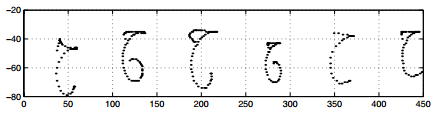
\includegraphics{./figures/ha_different}       
\caption{Different writing styles of the isolated form of the letter \RL{.h}.}
\label{fig:ha_different}
\end{figure}


%%%%%%%%%%%%%%%%%%%%%%%%%%%%%%%%%%%%%%%%%%%%%%
\subsection{Off-line versus On-line Handwriting Recognition}

\iftoggle{edit-mode}{\hspace{0pt}\marginpar{Introduction}}{}
The field of HWR can be classified in several ways. However, the most common categorization is the one that distinguishes between \emph{off-line} (also called static) and \emph{on-line} (also called dynamic).
Off-line HWR focuses on documents that have been written on paper at some previous point of time. A digital image of the document is fed to the computer, and the system attempts to convert the spatial representation of the letters into digital symbols \cite{al2011online}. 
In contrast, on-line HWR is performed on a digital representation of the text written on a special digitizer, tablet or smart-phone device, where sensors pick up the pen-tip movements and the two-dimensional coordinates of successive points of the writing as a function of time are stored.
Figure \ref{fig:offline_vs_online} shows typical input signals that can be analyzed in both cases.

\begin{figure}
	\centering
        \subfloat[]{
            \label{fig:offline}
            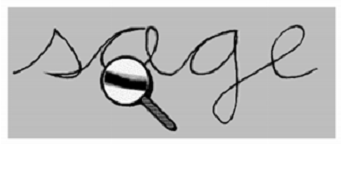
\includegraphics[width=0.5\textwidth]{./figures/offline}
        }
        \subfloat[]{
           \label{fig:online}
           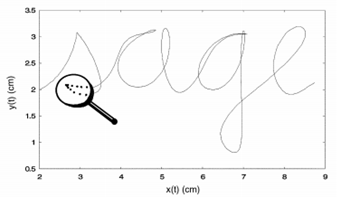
\includegraphics[width=0.5\textwidth]{./figures/online}
        }        
    \caption{An on-line vs. an off-line representation of a word \cite{plamondon2000online}.}
   \label{fig:offline_vs_online}
\end{figure}

\iftoggle{edit-mode}{\hspace{0pt}\marginpar{Literature}}{}
The research on on-line handwriting recognition started in the 1960's and has been receiving a great interest from the 1980's \cite{tagougui2013online}.
One of the earliest studies on On-line Arabic script recognition was carried out by El-Wakil and Shoukry in 1989 \cite{el1989line}.

\iftoggle{edit-mode}{\hspace{0pt}\marginpar{Similarities and advantages of on-line and off-line}}{}
Off-line HWR techniques can be applied to on-line data by constructing a static image of the on-line script. 
However, it has been shown that the information of the pen dynamics, such as the strokes breaking (i.e., "pen-down" and "pen-up" events) and the order of writing, can be used to obtain a better recognition accuracies than the static data alone. 
In the other direction, the success of on-line systems makes it attractive to consider developing off-line systems that first estimate the trajectory of the writing from the off-line data and then use on-line HWR techniques. 
Nevertheless, reconstructing the temporal data is problematic, and thus, has led to few such systems so far \cite{plamondon2000online}.

\iftoggle{edit-mode}{\hspace{0pt}\marginpar{off-line objectives}}{}
In general, off-line HWR systems are less accurate than on-line systems, but, they are now good enough that they have a significant economic impact on specialized domains such as interpreting handwritten postal addresses on envelopes and reading courtesy amounts on bank checks \cite{melin2007analysis}.

\iftoggle{edit-mode}{\hspace{0pt}\marginpar{A general flow for HWR}}{}
Despite the large variation among the different methods for HWR, there are several fundamental stages that are common between most of the systems.
The data acquisition step is the first stage in HWR. 
In the on-line case, the stylus motion is sampled at equal time intervals.
The samples go through a preprocessing stage that includes filtering of noises, re-sampling the stroke information to obtain equidistant stroke, and normalized to a standard size. 
Additional preprocessing may include slant and slope corrections. 
Then, depending on the nature of the system, the script may undergo segmentation into basic units that could be words, parts of words, single characters or graphemes.
Typically, a feature extraction technique is then applied to extract significant and distinguishing attributes of the input data.
Using a classification algorithm the basic units are labeled. 
In many cases, a post-processing stage is applied in which the language model is used to search for the most likely string in the lexicon.

\iftoggle{edit-mode}{\hspace{0pt}\marginpar{off-line HWR additional steps}}{}
Approaches for on-line and off-line handwriting recognition, while having much in common, are different, due to the disparity in the input data representation. 
Their different nature imposes different challenges and thus variable levels of efforts are required to be spent on the various stages.
The off-line HWR systems usually consist of additional steps of layout analysis and text lines extraction, which are activated at the beginning of the preprocessing stage. 
Each text line is then divided into words or WPs. 
The segmentation, in such system, is made into images that contain basic units. 
The whole process is straightforward for well printed or well written documents; however, in the case of historical or badly printed document much effort is invested in a preprocessing stage that include smoothing, writing flow reconstruction, purification, and more \cite{saba2010survey}. 

%%%%%%%%%%%%%%%%%%%%%%%%%%%%%%%%%%%%%%%%%%%%%%

\subsection{The Holistic versus the Analytic Approach}

\iftoggle{edit-mode}{\hspace{0pt}\marginpar{Importance of the dictionary size}}{}
The vocabulary, from which the words in the test set are taken, has a major impact on how difficult the HWR task is.

\iftoggle{edit-mode}{\hspace{0pt}\marginpar{Closed and open vocabulary definitions}}{}
Closed-vocabulary HWR systems are capable of recognizing words from a predetermined limited size dictionary. 
The restricted vocabulary set is usually called a lexicon.
There are no well-established criteria for the categorization of lexicon size. 
However, the following terms are usually used:
\begin{compactitem}
\item small lexicon - tens of words.
\item medium lexicon - hundreds of words.
\item large lexicon - thousands of words.
\item very large lexicon - tens of thousands of words.
\end{compactitem}
Open-vocabulary tasks refer to the recognition of any word without the constraint of being in a dictionary.

\iftoggle{edit-mode}{\hspace{0pt}\marginpar{Recognition difficulty}}{}
The lexicon is a key-point post-processing stage in many systems, because the linguistic knowledge helps to filter out many possible options that are not included in the lexicon, and consequently raises the recognition rate.
The adhesion to a limited dictionary, may also limit the computational complexity. 
Although most research efforts have been devoted to closed vocabulary systems, open vocabulary systems have also been proposed.
Yet, their accuracy is still far below those relying on a small vocabulary \cite{koerich2003large, shu1996line}.

\iftoggle{edit-mode}{\hspace{0pt}\marginpar{problems imposed by the open vocabulary}}{}
While there exists a wide variety of approaches to cursive script recognition, research in this field has established two main approaches, one is the analytic approach \cite{abdulla2008off, sari2002off, dinges2011offine, elanwar2012unconstrained}, and the other is the holistic approach \cite{biadsy2011segmentation}. 


The analytic approach involves segmentation of the input curve into basic units and the classification of each individual unit.
The advantage of this approach is that it requires to maintain only a small set of trained models - one for each letter shape - to handle large vocabulary. 
However, the absence of consistent baselines, large variations in writing styles, and seamless connection between letters (connection is done with almost no ligatures) makes segmentation into individual letters very challenging \cite{saabni2009hierarchical}.

\iftoggle{edit-mode}{\hspace{0pt}\marginpar{The holistic approach}}{}
The holistic approach considers the global properties of the written text and recognizes the input word shape as a whole. 
Most popular methods among this group are based on analysis of the number and order of ascenders, descenders, loops and vertical strokes; they often rely on heavy dictionary searching that is costly and prone to be mislead by spelling errors \cite{brodowska2011oversegmentation}.
While it avoids the error-prone segmentation process, in the holistic approach, the recognition system needs to be trained over all words in the dictionary and to maintain and train models for each word. 
Using the holistic approach may be possible for a small vocabulary of words, however, this is not feasible for large vocabularies (20,000 words or more). 
Since each word is constructed from a subset of the character alphabet, it is much more efficient to classify words using the analytic approach \cite{elanwar2012unconstrained}.
In addition, a survey done in \cite{al2011online} on Arabic HWR found that the analytic approach, in general, achieve higher recognition rates than the holistic systems, in cases where words are written in cursive manner, such in the Arabic script. 
This may lead us to conclude that segmentation is a crucial step and that the main problem recognizing Arabic text, especially its handwriting, is its cursiveness.

%%%%%%%%%%%%%%%%%%%%%%%%%%%%%%%%%%%%%%%%%%%%%%%%%%%%%%%

\subsection{Arabic Handwriting Recognition}

\iftoggle{edit-mode}{\hspace{0pt}\marginpar{The Arabic spread}}{}
The Arabic script is one of the descendants of the Aramaic script. 
The earliest known document written using the Arabic script dates from 512 AD.  
The Arabic language is spoken, as their first language, by nearly 350 million people around the world , and written by more than 100 million people, in over 20 different countries \cite{zeki2011segmentation}.
This makes it one of the five most common languages in the world and one of the six United Nations official languages since 1974 \cite{burrow2004arabic}. 
Although Arabic is used mainly in the Arab countries, which consists of about 5.5\% of the world population, almost all Muslims, around 25\% of the world population can read Arabic script as it is the language of the Holy Qur'an \cite{zeki2011segmentation}.

\iftoggle{edit-mode}{\hspace{0pt}\marginpar{The Arabic Alphabet usage in other languages}}{}
The use of Arabic language extended in the 7th and 8th centuries from India to the Atlantic ocean due to the Islamic conquests \cite{saabni2009efficient}. 
Consequently, more than twenty different languages adopted the Arabic alphabet with some changes. 
Examples of such languages are Farsi, Urdu, Malay, Housa and Ottoman Turkish.
Nevertheless, some of those languages has later adopted the Latin characters, but in general, people can still read the Arabic script \cite{zeki2011segmentation}.

\iftoggle{edit-mode}{\hspace{0pt}\marginpar{Literary vs. daily language}}{}
Although spoken Arabic is different from country to country, written Arabic is a standard system used all over the Arab world.
The literary language is called \emph{modern standard Arabic} or \emph{literary Arabic}, which it is currently the only official form of Arabic, used in most written documents as well as in formal spoken occasions, such as lectures and news broadcasts. 

\iftoggle{edit-mode}{\hspace{0pt}\marginpar{The growing interest in the Arabic HWR}}{}
The first work on Arabic character recognition is by Nazif \cite{nazif1975system} published in 1975, while the earlier research efforts in Latin may be traced back to the middle of the 1940s.
However, considerable increase in the number of research papers related to Arabic character recognition is evident in recent years.
The challenging nature of HWR has attracted the attention of researchers from industry and academic circles \cite{al2010development, zeki2011segmentation}.
A recent survey done by Tagougui et al. \cite{tagougui2013online} reviews the status of research in the on-line Arabic handwriting recognition field. 

%%%%%%%%%%%%%%%%%%%%%%%%%%%%%%%%%%%%%%%%%%%%%%%%%%%%%%%

\subsubsection{Characteristic of the Arabic Writing System}
\label{subsubsec:arabic_writing_characteristic}


\iftoggle{edit-mode}{\hspace{0pt}\marginpar{Basic properties}}{}
The Arabic script consists of 28 basic letters and is written from right to left in a semi-cursive manner in both printed and handwritten forms.
Most letters are written in four different letter shapes depending on their position in the word, e.g., the letter \RL{`}  (Ain) appears as \RL{`}  in its isolated form, \RL{`-} in its initial form, \RL{-`-} in its medial form and \RL{-`} in it final form. 
Among the basic letters, six are Dis-connective - \RL{A} /a/, \RL{d} /d/, \RL{_d} /th/, \RL{r} /r/  \RL{z} /z/ and \RL{w} /w/. 
Dis-connective letters do not connect to the following letter and have only two shapes each, isolated and final. 
The presence of these letters interrupts the continuity of the graphic form of a word. 
The parts of the word that are graphically connected are called \emph{word parts} (WPs). 
If the WP is composed of only one letter, this letter will be in its isolated shape \cite{biadsy2011segmentation}. 

\iftoggle{edit-mode}{\hspace{0pt}\marginpar{Delayed strokes}}{}
Certain characteristics relating to the obligatory dots and strokes of the Arabic script, distinguish it from Latin script.
These dots and strokes are called \emph{delayed strokes} since they are usually drawn last in the when scribing a WP or a word. 
There are mainly two types of delayed strokes, \emph{i'jam} (\RL{A`jAm}) and \emph{harakat} (\RL{.hrkAt}). 
The old Arabic was written without dots or diacritics. 
These additional strokes that were added to the Armaic letters, were first introduced around the 7th century, to prevent the Qur'an from being misread by Muslims \cite{burrow2004arabic}.

\iftoggle{edit-mode}{\hspace{0pt}\marginpar{I'jam}}{}
The i'jam are the pointing diacritics added to the main body of the letter (called rasm) and their role is to distinguish between various constants ,such as, the medial form letters \RL{-b-} /b/, \RL{-t-} /t/, \RL{-_t-} /s/, \RL{-n-} /n/, \RL{-y-} /y/.
Typically, i'jam are not considered diacritics but part of the letter and consists of one or more dots and lines added above, under or inside the letter.
Eliminating, adding or moving a i'jam produces a completely different letter and as a result a completely different word, thus, they are not omitted in the written documents.
Not only dots are used as i'jam, the \RL{'} (hamza) is another type of i'jam that distinguish between the letters \RL{k} /k/ and \RL{l} /l/ in their isolated and final forms.

\iftoggle{edit-mode}{\hspace{0pt}\marginpar{Harakat}}{}
The harakat are small markings added above or below the letters, are used to specify the exact pronunciation of the word.
These diacritics are used in the holy book Qur'an and are commonly used in teaching material and poetry but are seldom used in day-to-day communication and handwriting neither are much in use in the scientific, and business communication.

An example of a fully vocalised Arabic from the Qur'an (Al-Fatiha 1:1):

\begin{center}
\fullvocalize
\transtrue
\begin{RLtext}
bismi al-ll_ahi al-rra.hm_ani al-rra.hImi
\end{RLtext}
In the Name of All'ah, the Most Gracious, the Most Merciful...
\end{center}

\iftoggle{edit-mode}{\hspace{0pt}\marginpar{additional stroke}}{}  
In our work we recognize and classify the main body of the letter and ignore the additional stroke entirely. 
As a result, the number of different letters drops from 29 to 18.
It is important to note that taking the delayed strokes into consideration may be exploited to boost the classification rate.

\iftoggle{edit-mode}{\hspace{0pt}\marginpar{WP count}}{}    
Saabni and El-sana \cite{saabni2009efficient} have explored a large collection of Arabic texts and extracted 300,000 different word combinations of 82,000 different WPs.
Ignoring the delayed strokes, the number of different WP had reduced to 40,000. 

%\iftoggle{edit-mode}{\hspace{0pt}\marginpar{Challenges of the Arabic language}}{}  
%The main body of most Arabic letters is written by a single stroke. A single stroke can contain a single or multiple letters.
%However, there are some letters that usually written using two strokes, such as the letter \RL{-k-}  which is the middle form of the letter \RL{k} /k/. 
%The writer usually writes \RL{-l-} and adds the final upper slanted line when the main body is completed, as if he writes an additional stroke.
%Another problem arises when trying to recognize Arabic transcript, is that, different writers may write the main body of the same word part in a different number of strokes. 
%As can be seen very similar to the \RL{s} /s/ letter in its medial position \RL{-s-}, the only to distinguish between the two options is by looking at the additional strokes.
%For these mentioned complexities, when recognizing Arabic scripts, many researches have preferred the holistic approach. 
%%%%%%%%%%%%%%%%%%%%%%%%%%%%%%%%%%%%%%%%%%%%%%%%%%%%%%%


\subsection{Arabic Characters classification}
\iftoggle{edit-mode}{\hspace{0pt}\marginpar{The learning problem.}}{}
Classification is the problem of identifying to which of a set of classes an unlabelled observation belongs. 
In the case of \emph{supervised learning}, the classification is done based on a dataset of data containing labelled samples, referred to as the training set.
Given a domain space $X$, a target space $Y$ and a training set $S=\{(x_i,y_i)\}_{i=1}^{m}$ where $x_1,x_2,..,x_n\in X$ and $y_1,y_2,...,y_n \in Y$, we would like to find a function $h$, such that given an unlabelled point $x \in X$, $h$ will classify it correctly.


\begin{figure}
\centering
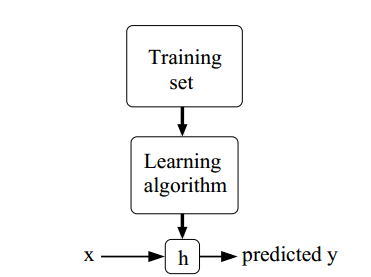
\includegraphics[width=0.5\textwidth]{./figures/machine_learning_diagram}       
\caption{A learning algorithm scheme}
\label{fig:machine_learning_diagram}
\end{figure}

\iftoggle{edit-mode}{\hspace{0pt}\marginpar{HWR Complexity}}{} 
Characters classification is a complex and challenging problems in the pattern recognition field.
This is due to the variation in characters shapes that result from variation in writing habits, styles, and the social and educational level of the writer.
Other factors which implicate the recognition is the variability of writing styles, cursive writing, text size differences and sampling issues, such as duplicate samples resulted from hesitate writers as well as non-adjacent consecutive samples caused by fast writers \cite{verma2004feature}.

\iftoggle{edit-mode}{\hspace{0pt}\marginpar{Letter classification using HMM}}{}
Many types of techniques were investigated for classifying Arabic characters, including Artificial Neural Networks \cite{alijla2012oiahcr}, Decision Trees \cite{ismail2012online}, $k$-NN \cite{elglaly2011isolated} and Hidden Markov Models (HMMs). 
Particularly, HMMs has gained a vast amount of studies done in the field of HWR \cite{pechwitz2003hmm, khorsheed2003recognising, al2007combination, benouareth2008arabic, mahmoud2008recognition, shu1996line, biadsy2006online}. 

While having many advantages, the HMM makes some powerful assumption about the data that may not necessarily true, such as the Markovian assumption which presumes that the transition probabilities depend only on the current state \cite{kadous2002temporal}. 
In addition, HMMs require a large amount of data for its training.

\iftoggle{edit-mode}{\hspace{0pt}\marginpar{The k-NN classifier}}{}
The $k$-nearest neighbours algorithm ($k$-NN) is a well-known classification technique in supervised learning. 
It predicts the query objects class memberships based on the $k$ closest training examples. 
The $k$-NN algorithm is one of the simplest of all machine learning algorithms: an object is classified by a majority vote of its neighbours, with the object being assigned to the class most common amongst its k nearest neighbours ($k$ is a positive integer, typically small). 
If $k=1$, then the object is simply assigned to the class of that single nearest neighbour. 
In many cases, the notion of distance between objects is obvious, however in many other interesting cases it cannot be easily defined.
On the one hand, beside its simplicity, $k$-NN has some major advantages. 
$k$-NN is especially a good learning method for complex target functions.  
On the other hand, the $k$-NN algorithm has some drawbacks. 
First, $k$-NN needs a large dataset in-order to achieve high classification accuracy. 
Second, it is very sensitive to data errors and can be easily fooled by outliers.

\iftoggle{edit-mode}{\hspace{0pt}\marginpar{Literature review}}{}
An on-line Arabic handwritten character recognition method, which uses structural features and decision trees, was presented by Al-Taani and Al-Haj \cite{al2010recognition}. 
The system was tested on a set of 1400 different characters and achieved about 75\% recognition rate. 
The dataset was obtained by capturing the handwriting of 10 users that wrote the 28 Arabic characters, in their isolated form, five times in order.
A rules based approach for on-line Arabic characters classification was proposed in \cite{ismail1859online}. 
The performance of the system was compared to the classification results obtained using artificial neural networks and and decision trees. 
A set of 504 characters were used for training and the test set contained 336 characters. 
The system obtained a recognition rate of about 97\%. 
Addakiri and Bahaj \cite{addakiri2012line} presented an on-line Arabic handwritten character
recognition system based on Neural Networks. 
Their approach was tested on 1400 different characters written by 10 users and achieved accuracy of 83\%.

\subsection{Arabic Script Segmentation}
\iftoggle{edit-mode}{\hspace{0pt}\marginpar{Introduction}}{}
An integral part of the handwriting recognition process, when the analytic approach is considered, is segmentation. 
Therefore, it has long been a critical area of the OCR process. 
As for many pattern recognition problems, the task of segmentation, while usually trivial to a human to perform, is a very challenging pattern recognition problem.
Segmentation and recognition of cursive text are two tasks intertwined and dependent on each other. 
It is believed that wrong segmentation will often result in a major contribution to the error of the recognition algorithm \cite{brodowska2011oversegmentation}. 
But, in order to determine the segmentation, the system may try to seek a pattern that will match a member of the system's alphabet \cite{casey1996survey}.
The segmentation task of cursive and unconstrained nature of languages such as Arabic, makes the segmentation task even harder.  
Several segmentation approaches have been proposed in the literature for Arabic OCR, yet, correct and efficient segmentation of the Arabic text is not easily achievable and considered to be a challenging problem even for printed text. 

\iftoggle{edit-mode}{\hspace{0pt}\marginpar{The context dependent of segmentation}}{}
A reliable recognition system requires more than a good matching to a set of letters symbol classes.
The segmentation decision is not a local decision and may affect subsequent segmentation decisions, thus, a poor match of the current segment to some class in the letter library can cast doubt on the correctness of the future segmentation decisions.
In addition, even a series of satisfactory pattern matches can be judged incorrect if contextual requirements of the system output are not satisfied \cite{casey1996survey}.
For instance, in handwritten English, the letter combination "cl" is graphically similar to the letter "d", but in some cases contextually not valid.
In Arabic, two or three consequent appearances of rasm \RL{-b-} /b/ (that is common for the letters \RL{-y-} /y/, \RL{-t-} /t/ and more, see Section \ref{subsubsec:arabic_writing_characteristic}) are very similar to the \RL{-s-} /s/ letter. 
The only way to distinguish between the two options is by considering the delayed strokes and the contextual validity.

\iftoggle{edit-mode}{\hspace{0pt}\marginpar{Approaches for segmentation}}{}
In a comprehensive survey done in \cite{casey1996survey}, the authors pinpointed two elemental strategies for off-line cursive text segmentation in addition to many approaches that are combinations of these three. 
They have noted that much of the literature on segmentation reports methods that can be characterized as a blend of these three mentioned methods.

\iftoggle{edit-mode}{\hspace{0pt}\marginpar{Dissection}}{}
The first strategy is the classical approach, which is usually named \emph{dissection}, attempts are made to segment the text into primitives. 
Dissection techniques attempt to find appropriate candidate points by learning the characteristic of the segmentation point or by using a rules-based engine. 
Segments, that result from the segmentation process, do not necessarily correspond to exactly one character. 
The word could be segmented into components called graphemes, which are a combination of two or three letters, or a part of a letter. 
The relationship between graphemes and letters is applied in a later phase. 
Many morphological properties were exploited for this task, such as, height, width, separation from neighboring components, low slope if the candidate point local environment, etc.
Various strategies such as projection profile, bounding box or contour tracing exhibit promising results. 
Different types of scripts with essential distinctive nature usually require using different type of properties.
For instance, local minima in the upper or lower contour is commonly used for segmenting English cursive script but not in the Arabic script. 
Such approaches can segment typical words accurately, but, might lead to incorrect segmentation when deal with unconstrained cursive handwriting \cite{saba2010survey}.
A common approach that is followed by many researchers is first over-segmenting of the text, i.e, finding some set of potential splitting points that partition the handwritten word into primitives and then be processed further to eliminate improper candidates point \cite{daifallah2009recognition}.

\iftoggle{edit-mode}{\hspace{0pt}\marginpar{Recognition-based segmentation}}{}
The second approach is the recognition-based segmentation, in which the system searches for sub-components in the cursive text that match letters in its alphabet. 
As mentioned before, character segmentation and character classification are not totally separate steps with a varying degree of dependency.
The initial selection of points can be made in a variety of methods. 
For example, using a moving window with a predefined width which breaks the word into many overlapping pieces without regard to its content.
Then, an iterative or parallel recognition method is used to search for "satisfactory" classification scoring for joint sub-components usually by generating a lattice of all or many possible combinations of the initial candidates set. 
The final decision is determined by the best path through the lattice. 
While avoiding using complex dissection methods, such techniques rely heavily on the classifier accuracy which heavily affects the overall segmentation accuracy \cite{casey1996survey}.

\iftoggle{edit-mode}{\hspace{0pt}\marginpar{Literature Review}}{}
Randa et al. \cite{elanwar2012unconstrained} proposed a two stage on-line Arabic handwritten text segmentation system based on Hidden Markov Model (HMM). 
In the first stage, SPs were nominated, and then, in a second stage, the nominated points were validated using a rules-based engine. 
The system was tested using a self-collected database named OHASD.
Segmentation-based recognition approach based on dividing the word into smaller pieces was proposed in \cite{dinge2011offine}. 
The words were afterwards segmented into candidate letters, and then classified into letter classes, using statistical and structural features. 
A $k$ nearest neighbor ($k$-NN) classifier was used to obtain the final recognition.
A segmentation-based recognition method that operates on the stroke level for on-line Arabic handwritten words recognition was proposed by Daifallah et al. \cite{daifallah2009recognition}. 
SPs were nominated and then selected by locating semi-horizontal lines moving from right to left. 
A portion of the SPs is filtered out by applying a certain set of rules. 
Then, HMM is used to classify the sub-strokes to letters using the Hu feature. 
The letters candidates and their scoring were used to determine the best set of SPs.

%%%%%%%%%%%%%%%%%%%%%%%%%%%%%%%%%%%%%%%%%%%%%%%%%%%%%%%
\newpage{}
%%%%%%%%%%%%%%%%%%%%%%%%%%%%%%%%%%%%%%%%%%%%%%%%%%%%%%%


\section{Thesis Scope and Outline}

In this thesis, we propose and implement a novel real-time approach for segmenting and recognizing on-line handwritten Arabic script.
In Chapter \ref{chap:characters_classification}, we present a fast technique for Arabic characters classification.
The characters classifier employs state-of-the-art similarity measure and search techniques for fast and accurate classification of characters.

A real-time, stroke level, recognition-based, segmentation technique is detailed in Chapter \ref{chap:strokes_segmentation}.
We present a procedure for nominating segmentation points whilst the stroke is being scribed and proposed algorithms for selecting the final segmentation set of segmentation points.
The results obtained by the classification system and the segmentation process are presented in Chapter \ref{chap:results}.
A summary and planned future work are given in Chapter \ref{chap:summary}. 

The ADAB is a de-facto a standard database providing a large dataset of on-line Arabic handwritten samples.
Extracting letter samples from the ADAB database required us to develop a system that enables a human expert to manually segment word samples and produce an Arabic character sample set that can be used in future research. 
An overview on the manual segmentation system and a description of the resulted characters database is given in Appendix \ref{app:data_collection}.
A brief explanation on wavelets and the wavelet transform is provided in Appendix \ref{app:wavelets}. 

The system is based on assumptions and has limitations.
First, it does not regard additional strokes although they can be used to improve the classification results.
Second, the analysis is performed independently on each stroke thus the system does not handle letters spanned over multiple strokes. 
While this is a reasonable assumption, it is not always true. 
Our future work will focus on waiving these limitations. 

%%%%%%%%%%%%%%%%%%%%%%%%%%%%%%%%%%%%%%%%%%%%%%%%%%%%%%%
\newpage{}
%%%%%%%%%%%%%%%%%%%%%%%%%%%%%%%%%%%%%%%%%%%%%%%%%%%%%%%

\section{Conference Publications}

The results of this research have been concluded and published in two conference papers.  

\begin{itemize}

\item A paper titled \emph{"Fast Classification of Handwritten On-line Arabic Characters"} was accepted for publication in the proceedings of the \emph{6th International Conference of Soft Computing and Pattern Recognition} (SoCPaR 2014) in June 20, 2014.

\item A conference paper titled \emph{"Real-time Segmentation of On-line Handwritten Arabic Script"} was accepted for publication in the proceedings of the \emph{14th International Conference on Frontiers in Handwriting Recognition} (ICFHR-2014) in April 21, 2014.

\end{itemize}



%\bibliographystyle{plainnat}
%\bibliography{references}
%\end{document}

%\documentclass[12pt,english]{report}
%\usepackage{mathptmx}
%\renewcommand{\familydefault}{\rmdefault}
%\usepackage[T1]{fontenc}
%\usepackage[latin9]{inputenc}
%\usepackage[a4paper]{geometry}
%\setcounter{secnumdepth}{2} % Changed from 3 to 2. 0-chapter 1-section 2-subsection 
%\setcounter{tocdepth}{2} % Changed from 3 to 2. 0-chapter 1-section 2-subsection 
%\setlength{\parskip}{\medskipamount}
%\setlength{\parindent}{0pt}
%\usepackage{verbatim}
%\usepackage{pdfpages}
%\usepackage{graphicx}
%\usepackage{subfig} %% This package has to be here
%\usepackage{setspace}
%\usepackage{arabtex}
%\usepackage[numbers]{natbib}
%\usepackage{nomencl}
%\usepackage{paralist}
%\usepackage{amsthm}
%\usepackage{amsmath}
%\usepackage{amsfonts}
%\usepackage{etoolbox}
%\newtoggle{edit-mode}
%\togglefalse{edit-mode}  
%\toggletrue{edit-mode}
%\iftoggle{edit-mode}{
%\geometry{verbose,tmargin=2cm,bmargin=2cm,lmargin=2cm,rmargin=6cm,headheight=1cm,headsep=1cm,footskip=1cm, marginparwidth=5cm}
%}{
%\geometry{verbose,tmargin=2cm,bmargin=2cm,lmargin=2cm,rmargin=2cm,headheight=1cm,headsep=1cm,footskip=1cm}
%}
%
%\makenomenclature
%
% %Theorem Styles
%\newtheorem{theorem}{Theorem}[section]
% %Definition Styles
%\theoremstyle{definition}
%\newtheorem{definition}{Definition}[section]
%\newtheorem{example}{Example}[section]
%\theoremstyle{remark}
%\newtheorem{remark}{Remark}
%
%\usepackage[linesnumbered]{algorithm2e}
%
%\begin{document}
%
%\tableofcontents{}

%%%%%%%%%%% nomenclature %%%%%%%%%%
\nomenclature{SC}{Shape Context}
\nomenclature{MAD}{Multi Angular Descriptor}
\nomenclature{PCA}{Principal Component Analysis}
\nomenclature{LDA}{Linear Discriminant Analysis}
\nomenclature{DTW}{Dynamic Time Warping}
\nomenclature{EMD}{Earth Mover's Distance}
\nomenclature{LSH}{Locality Sensitive Hashing}
%%%%%%%%%%%%%%%%%%%%%%%%%%%%%%%%%%%%


\chapter{Fast Classification of On-line Handwritten Arabic Characters}
\label{chap:characters_classification}

\iftoggle{edit-mode}{\hspace{0pt}\marginpar{The learning process}}{}
Letter samples extracted from the ADAB databases were split into four groups according to their position: \textbf{Ini}, \textbf{Med}, \textbf{Fin} and \textbf{Iso}. 
The set of samples in each position undergone a learning process that contains five main stages.
First, the samples were preprocessed as described in Section \ref{sec:preprocessing}.
Second, feature vectors were extracted as detailed in Section \ref{sec:feature_extraction}.
Then, the feature vectors were embedded into the $L_1$ metric space by extracting the scaled coefficients of the wavelet transformation, as presented in Section \ref{sec:similarity_search}.
This was done to enable fast computation of intuitive similarity search techniques, described in Section \ref{sec:similarity_measures}.
In Section \ref{sec:dr}, we outline a dimensionality reduction process that obtains a compact representation of the high dimensional vectors produced by the embedding procedure.
In the last stage, described in Section \ref{sec:metric_indexing}, we build a metric index that enables finding the most similar object in sub-linear time.

\iftoggle{edit-mode}{\hspace{0pt}\marginpar{The recognition process}}{}
The classification process corresponds to the learning process.
Given an un-labelled query sequence, the sequence undergoes preprocessing, features extraction, embedding and dimensionality reduction.
The low dimensional vector is then used to to find the closest ten sample among the large list of sample containing more than a thousand instances.
As described in Section \ref{sec:candidates_scoring}, we then allow the usage of an accurate and expensive similarity measure technique to rank the short list of candidates. \\
An overview of the learning and classification processes is given in Figure \ref{fig:classification_system_flow}.

\begin{figure}
\centering
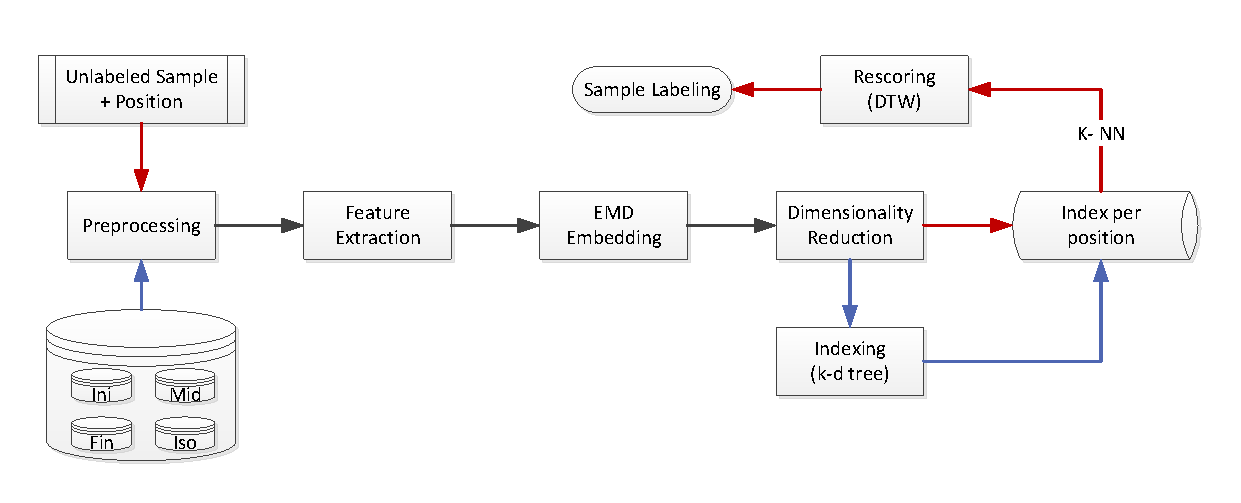
\includegraphics[width=1\textwidth]{./figures/classification_system_flow}
\caption{High level diagram of both the training and classification flows. The blue arrows indicate parts that are unique to the training process and the red arrows indicate parts that are unique to the classification process.}
\label{fig:classification_system_flow}
\end{figure}


%Thus a re-scoring stage using a costly but accurate similarity measure is applied on a short list of candidates.   
%The scoring of candidates based on the approximate EMD metric may not sufficiently precise for application that use the this scoring to perform delicate analysis tasks, such as the recognition-based segmentation approach described in Chapter \ref{chap:strokes_segmentation}.

%%%%%%%%%%%%%%%%%%%%%%%%%%%%%%%%%%%%%%%%%%%%%%%%%%%%%%%
\newpage{}
%%%%%%%%%%%%%%%%%%%%%%%%%%%%%%%%%%%%%%%%%%%%%%%%%%%%%%%

\section{Samples Preprocessing}
\label{sec:preprocessing}

\iftoggle{edit-mode}{\hspace{0pt}\marginpar{Introduction}}{}
Digitizers tend to generate a jagged and non-uniform sampling of the trajectory scribed on their surface.
Such devices, normally, sample the input in constant time intervals, thus, slow pen motion regions are over-sampled and fast motion regions are under-sampled.
Further imperfections are caused by hand vibrations resulting from hesitant writing \cite{huang2009preprocessing}.
This lack of uniformity in the data, if not deliberately used by the classification system, should be reduced to avoid negative influence the classification system performance.
In order to overcome the flaws mentioned, preprocessing operations are usually needed to impose certain uniform structure on the data, to comply with the input structure required for the proper operation of the subsequent parts of the system \cite{al2011online}.

\iftoggle{edit-mode}{\hspace{0pt}\marginpar{Preprocessing steps usage}}{}
In the current work, preprocessing consists of three methods: \textbf{normalization}, \textbf{noise elimination} and then \textbf{re-sampling}.
While these three techniques were applied in the mentioned order in both learning and classification of letters, these steps were selectively activated in the segmentation system according to the needs of the specific step.
Other less commonly used preprocessing steps in the field of on-line Arabic HWR, such as rotation and slant normalization \cite{jaeger2001online}, were not implemented in this work. 


\subsection{Normalization}
\iftoggle{edit-mode}{\hspace{0pt}\marginpar{Goal}}{}
Size normalization is performed to achieve a uniform size of the bounding box surrounding the pattern. 
It was applied on each sequence so that it will fit into a $[0,1]\times[0,1]$ bounding box without affecting the original aspect ratio. 
This stage includes an additional step of translating the sequence so that the sequence's center of gravity is located in the origin point, i.e., at $[0,0]$.
Although the features used in this work are agnostic to the pattern's size and location, this step is mostly required by the segmentation flow.

\iftoggle{edit-mode}{\hspace{0pt}\marginpar{Approach}}{}
Given the stroke sequence $S=\{p_i\}_{i=1}^{n}=\{(x_i,y_i)\}_{i=1}^{n}$, the normalized sequence $\bar{S}=\{\bar p_i \}_{i=1}^{n}=\{(\bar x_i,\bar y_i)\}_{i=1}^{n}$ is calculated by: 
\begin{equation}
{\bar x_i} = {{\left( {{x_i} - {\mu _x}} \right)} \over W},{\bar y_i} = {{\left( {{y_i} - {\mu _y}} \right)} \over W}
\end{equation}
where $W = \max (d_x,d_y)$, $d_x$ and $d_y$ are the width and hight of the sequence, respectively, and $\mu$ is the center of gravity of the it, i.e., 
\begin{equation}
\mu  = \left( {{\mu _x},{\mu _y}} \right) = \left( {{1 \over N}\sum\limits_{i = 1}^N {{x_i}} ,{1 \over N}\sum\limits_{i = 1}^N {{y_i}} } \right)
\end{equation}


\subsection{Noise Elimination}

\iftoggle{edit-mode}{\hspace{0pt}\marginpar{Introduction}}{}
The input obtained by the digitizer usually contains a large amount of noise irrelevant for pattern classification. 
This noise consists mainly of redundant points duplication and inadequacies caused by hand vibrations. 
The \emph{Douglas-Peucker Polyline Simplification} algorithm described in \cite{douglas1973algorithms}, also known as the \emph{Iterative Endpoint Fit} algorithm, was used for eliminating such deficiencies in the data. 

\iftoggle{edit-mode}{\hspace{0pt}\marginpar{The Douglas-Peucker algorithm}}{}
The algorithm reduces the number of vertices in a piecewise linear curve, given a pre-set tolerance parameter $\varepsilon$, which defines the maximum 'dissimilarity' between the original and the reduced curve.
It outputs a simplified curve, that consists of a subset of the points in the original curve.
The algorithm operates as follows. 
Initially, it marks the first and the last points to be kept, then it finds the furthest point, $p$, from the line segmented with the first and last points as end points.
If the distance is smaller that $\varepsilon$, the algorithm returns. 
Otherwise, $p$ is kept, and the algorithm recursively operates on the the first point and $p$ and then with $p$ and the last point.
When the recursion is completed, the kept points define an angular skeletonization of the original curve.

\iftoggle{edit-mode}{\hspace{0pt}\marginpar{Different tolerance parameters}}{}
In the normal preprocessing flow, in which normalization is done prior to the simplification process, we empirically set $\varepsilon  = {1 \over 75}$.
However, in cases where normalization is not applicable, such as in the segmentation system, the tolerance parameter has to be dependent on the the pattern's un-normalized bounding box area. 
In such cases, the tolerance parameter was set to: $\varepsilon  = {1 \over {200}}\sqrt {{d_x}^2 + {d_y}^2}$, where $d_x$ and $d_y$ are the width and height of the pattern, respectively. 
The division factors of both cases were tuned empirically. 
The discrepancy in the division factors can be explained by the difference in the sensitivity required in the two flows. 

\subsection{Re-sampling}
\iftoggle{edit-mode}{\hspace{0pt}\marginpar{Goal}}{}
The simplification process produces a highly angular, and non-uniform distribution of points along the stroke trajectory.
Naturally, there are less points in straight areas and a higher density of points in the curved areas stroke. 
This stage, using splines interpolation method, we produce an equidistant smoothed data sequence for a given re-sampling target number of points, $R$. 

\iftoggle{edit-mode}{\hspace{0pt}\marginpar{Approach}}{}
Given a stroke $S=\{(x_i,y_i)\}_{i=1}^{n}$, let $f_{x}(d)$ and $f_{y}(d)$ be the quadratic piecewise interpolations function of $\{x_i\}_{i=1}^{n}$ and $\{y_i\}_{i=1}^{n}$, respectively. 
$f_{x}(d)$ and $f_{y}(d)$ are functions of the coordinate values with respect to the arc-length distance from the pattern's starting point. 
Let $t_i=i\frac{L}{R}$ for $i=0,...,R$ where L is the arc-length of the pattern.
The re-sampled sequence is given as follows:
\begin{equation}
\widehat{S}=\{(f_x(t_i),f_y(t_i))\}_{i=1}^{R}
\end{equation}
Figure \ref{fig:before_after_preprocessing} demonstrates the pre-processing steps applied on a handwritten letter sample.
In our case, we set $R=40$.

\begin{figure}
	\centering
        \subfloat[]{
            \label{fig:preprocessing_orig}
            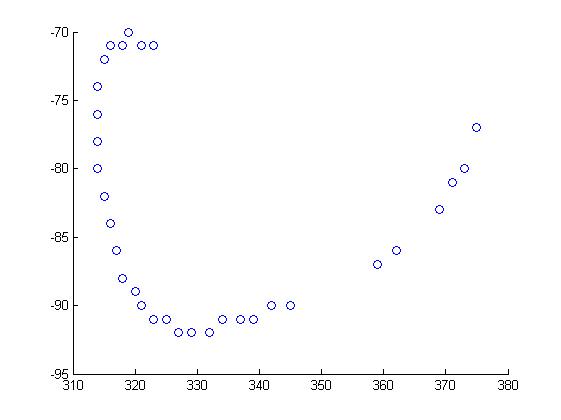
\includegraphics[width=0.4\textwidth]{./figures/preprocessing_orig}
        }
        \subfloat[]{
           \label{fig:preprocessing_norm}
           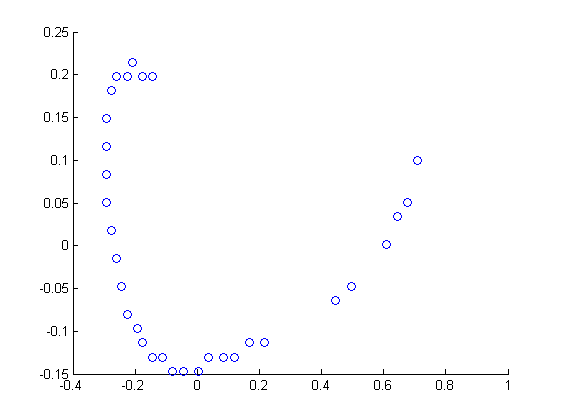
\includegraphics[width=0.4\textwidth]{./figures/preprocessing_norm}
        }  \\
        \subfloat[]{
            \label{fig:preprocessing_simpl}
            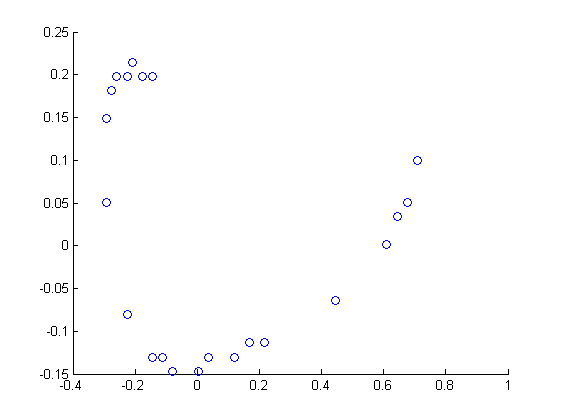
\includegraphics[width=0.4\textwidth]{./figures/preprocessing_simpl}
        }
        \subfloat[]{
           \label{fig:preprocessing_resamp}
           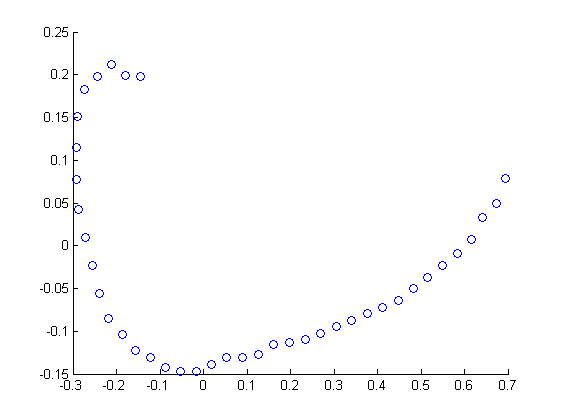
\includegraphics[width=0.4\textwidth]{./figures/preprocessing_resamp}
        }       
    \caption{A sample of the character \RL{b} before preprocessing (\ref{fig:preprocessing_orig}); after normalization (\ref{fig:preprocessing_norm}); after noise elimination (\ref{fig:preprocessing_simpl}) and after re-sampling (\ref{fig:preprocessing_resamp}).}
   \label{fig:before_after_preprocessing}
\end{figure}


%%%%%%%%%%%%%%%%%%%%%%%%%%%%%%%%%%%%%%%%%%%%%%%%%%%%%%%
\newpage{}
%%%%%%%%%%%%%%%%%%%%%%%%%%%%%%%%%%%%%%%%%%%%%%%%%%%%%%%

\section{Shape Descriptors}
\label{sec:feature_extraction}
\iftoggle{edit-mode}{\hspace{0pt}\marginpar{Feature extraction}}{}
Feature extraction is the process of extracting informative parameters for learning and recognition of patterns. 
Poor feature extraction and selection will, in most cases, result in a poor system performance, regardless of the sophistication of the classification algorithm \cite{parizeau2001character}.
The transformation to the feature space is done by extracting descriptive and expressive information from the raw data representation. 
A desired feature extraction technique should facilitate assessing the similarity degree between two objects by maintaining that the distance between them in the feature space reveals their similarity in the real world, and to do so inexpensively.

\iftoggle{edit-mode}{\hspace{0pt}\marginpar{Introduction - Cont.}}{}
In the field of image retrieval and off-line text recognition, the input data is too large and tends to be redundant, thus, feature extraction techniques are used to reduce the representation of the input data. 
However, in the case of recognising on-line handwritten shapes, the input data are compact and feature extraction techniques create feature vector referred to as the \emph{shape descriptor}, which offer discriminative characterization that capture the perceptual dissimilarity between two shapes. 
Unlike the first case in which the features extraction process is a form of data representation reduction, the raw amount of data contained in the shape descriptors usually exceeds the amount of data in the original input data.

\iftoggle{edit-mode}{\hspace{0pt}\marginpar{Shape Descriptors}}{}
Effective shape descriptor must have some essential properties such as invariance under translation, rotation and scale. 
A desirable shape descriptor should have a compact representation and must be easy to compute \cite{zhang2004review}.
It also have to be robust to noise so that distorted shapes which are tolerated by human beings when comparing shapes should be endured also by the shape descriptor \cite{zhang2004review, kim2000region}.

\iftoggle{edit-mode}{\hspace{0pt}\marginpar{Shape descriptors types}}{}
A common classification of shape descriptors is to local and global descriptors. 
Local descriptors calculate a given feature independently at each sample point. 
An example for a simple local feature is the vector containing the tangent slope angle for every given point in the sample point.
Descriptors such as cusps, crossings and loops are referred to as global descriptors and are calculated on the entire shape \cite{hu1997combining}. 
For a comprehensive review on shape descriptors see \cite{zhang2004review} and \cite{yang2008survey}.

\iftoggle{edit-mode}{\hspace{0pt}\marginpar{Using off-line shape descriptors for on-line HWR}}{}
Many of the well known and powerful feature sets operate on the shape's contour.  
However, the input data in the on-line case is a sequence of points representing the pattern trajectory and no contour is involved. 
Using feature sets that were originally developed for contours for recognizing contour-less shapes is common. 
Saabne and El-Sana employed the \emph{Shape Context} (SC) descriptor, a global shape descriptor that was originally developed for contour based shapes, for on-line handwriting recognition in \cite{saabni2009hierarchical}. 
Another example is the usage of the \emph{Multi scale shape context} for on-line handwritten mathematical expressions segmentation in \cite{husegmenting}. \\
In this work we employed and compared two shape descriptors, the SC descriptor and the \emph{Multi Angular Descriptor} (MAD). 

\iftoggle{edit-mode}{\hspace{0pt}\marginpar{Shape Context}}{}
The SC descriptor was presented by Belongie and Malik in \cite{belongie2002shape}.
Given a sequence of points $S=\{p_i\}_{i=1}^n$, the descriptor of the point ${p_i}$, is the coarse histogram of the relative coordinates as defined in Equation \ref{eq:sc_bins}.
The basic idea of the SC descriptor is illustrated in Figure \ref{fig:shape_context_demo}. 
\begin{equation}
{h_i}(k) = \# \{q \ne p_i:(q - p_i) \in bin(k) \}
\label{eq:sc_bins}
\end{equation}
The SC vector of the entire pattern is defined as the concatenation of all the point descriptors.
The bins are normally taken to be uniform log-polar space, making the descriptor more sensitive to positions of nearby sample points than to those of points farther away. 

\begin{figure}
\centering
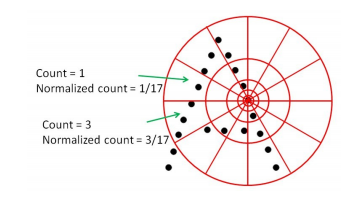
\includegraphics[width=0.3\textwidth]{./figures/shape_context_online}   
\caption{Diagram of the log-polar bins used to compute the Shape Context.}
\label{fig:shape_context_demo}
\end{figure}

\iftoggle{edit-mode}{\hspace{0pt}\marginpar{MAD}}{}
The other shape descriptor used in this thesis is the MAD, which was proposed by Saabne in \cite{saabni2013multi}. 
It captures the angular view from multi resolution rings in different heights. 
The shape is treated as a two dimensional set of points and the different rings are upper view points from rings around the shape centroid with different sizes and heights. 
To enable scale and translation invariance, the sizes and heights of these rings are calculated using the diameter and centroid of the shape.
Formally, let $S$ be a shape and Let $C$ and $D$ be the centroid and the diameter of the shape respectively. 
Let $S = \{p_j\}_{j = 1}^n$ a set of $n$ point taken uniformly on the shape. 
Let $R$ be a ring with the radius $r$ and the center $C$ positioned above the shape $S$ with the height $h$. 
Let $V = \{V_i\}_{i = 1}^\ell$ be a set of $\ell$ viewpoints lying uniformly on the ring $R$ and $\alpha(V_{ij})$ to be the angle between the segment $\overline {{V_i}{p_j}}$ and the plain contains the shape $S$. 
When the parameter $j$ goes over all points in the sequence, we get the vector $Vec_i$ describing the shape from the view point $V_i$.
The descriptor is the concatenation the vectors $V_i$ when the parameter $i$ goes over all viewpoints. 
See illustration in Figure \ref{fig:mad_demo}.

In Section \ref{sec:classification_results} we compare the performance of the above descriptors in our implementation. 

\begin{figure}
\centering
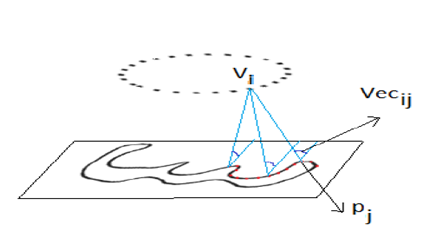
\includegraphics[width=0.5\textwidth]{./figures/mad_demo}       
\caption{A visual demonstration of the Multi Angular Descriptor feature set \cite{saabni2013multi}.}
\label{fig:mad_demo}
\end{figure}

%%%%%%%%%%%%%%%%%%%%%%%%%%%%%%%%%%%%%%%%%%%%%%%%%%%%%%%
\newpage{}
%%%%%%%%%%%%%%%%%%%%%%%%%%%%%%%%%%%%%%%%%%%%%%%%%%%%%%%

\section{Similarity Measures}
\label{sec:similarity_measures}

\iftoggle{edit-mode}{\hspace{0pt}\marginpar{Introduction}}{}
Given two visual data elements, the task of mathematically capturing the human perceptual similarity between them is extremely challenging. 
Similarity measure algorithms aim to quantitatively approximate the perceptual resemblance between data elements. In this chapter, we overview and discuss the different aspects of similarity measure evaluation techniques and present two approaches used in this work.

\iftoggle{edit-mode}{\hspace{0pt}\marginpar{Intuition}}{}
$k$-NN based classification techniques require the ability to correctly and efficiently determine the perceptual distance between two given objects.
Evaluating the dissimilarity between two handwritten strokes based on the raw data representation is difficult and computationally expensive. 
To overcome this hardship, feature extraction methods are used, as described in Section \ref{sec:feature_extraction}, to map the original data into the feature space.  
The similarity measure is formalized as a \emph{distance function}. 
\begin{definition}
Given a data space $\mathfrak{D}$, for any two data elements $x,y \in \mathfrak{D}$, a \textbf{distance function} $dist$, on $\mathfrak{D}$ is defined as:
\begin{equation}
dist: \mathfrak{D} \times \mathfrak{D} \longrightarrow \mathds{R}_{\geq 0} 
\end{equation}
where $dist$ has the following properties:
\begin{compactitem}
\item $dist(x,y)=0 \Leftrightarrow x=y$ (reflexivity)
\item $dist(x,y) = dist(y,x)$ (symmetry)
\end{compactitem}
The pair $(\mathfrak{D},dist)$ is called a \textbf{distance space}.
\label{def:distance_function}
\end{definition}

\iftoggle{edit-mode}{\hspace{0pt}\marginpar{Properties of a good dissimilarity measure.}}{}
The distance function should be carefully designed to best suit the application and the data representation it handles.
A good similarity measure should be able to cope with various types of discrepancy which can be easily handled by a human such as shifting, noise and scaling. Time shifting may be caused by different sampling rate and noise may be introduced by sensor failures or variations \cite{chen2005similarity}.\\
Significant amount of research has been carried out on similarity measure methods, in terms of defining the appropriate distance function and their efficient evaluation. 
Much research was done on similarity measure of time series and distributions. 
In this work, despite the fact we do not consider the temporal information of the written stroke we use a distance function that was originally designed for time series.

\iftoggle{edit-mode}{\hspace{0pt}\marginpar{Euclidean and Manhattan}}{}
The Euclidean distance is a basic, common and easy to compute distance function. 
Yet, it is not necessarily appropriate for capturing distances in any given space. 
For instance, a taxi driver in Manhattan should not measure the distance in terms of the straight line length to his destination, but needs to take into account that streets are either orthogonal or parallel to each other.
The Euclidean and the Manhattan distances, are special cases of the \emph{Minkowski} distance.

\iftoggle{edit-mode}{\hspace{0pt}\marginpar{Different Representations}}{}
Generally, similarity measure techniques can be applied on the raw data or on other representations of the data, such as on the feature vectors \cite{chen2005similarity}. 
Usually, different similarity measure methods are used for different types and representations of the data. 
The distance between two objects with a relatively complex mathematical construct are usually defined based on the distance function of its basic elements. 
For example, the distance between two vectors, will be defined using the distance function of two numbers. 

\iftoggle{edit-mode}{\hspace{0pt}\marginpar{Drawbacks of the Minkowski distance}}{}
The Minkowski distance is brittle and has several disadvantages when applied on stroke trajectories.
First, it requires the two sequences to be of the same length. 
One could add padding zeros to the shorter sequence to overcome this problem, but it would harm the similarity measure nonetheless. 
Second, it does not support local shifting, which occurs when one point of one sequence is shifted to match an element of the other sequence (even when the two matched elements appear in different positions in the sequences). 
It is important to consider these local shifts especially when the compared sequences have similar shape but are out of phase. 
It is called "local", because not all of the points of one sequence need to be shifted in the same factor and direction to match the other sequence. 
By contrast, "global" shifting is the case in which all points are shifted along the same direction by a fixed shifting factor. 
Generally, local and global shifting cannot be handled effectively by Minkowski distance \cite{chen2005similarity}.

\iftoggle{edit-mode}{\hspace{0pt}\marginpar{Metric Definition}}{}
The Minkowski distance function is a \emph{metric}. Mathematically, metrics are a generalization of the Euclidean distance, keeping some of its well-known geometric properties. 
These convenient properties facilitate utilizing efficient data structures and search algorithms. A formal definition of a metric is given in Definition \ref{def:metric_function}.

\begin{definition}
Given a data space $\mathfrak{D}$, a distance function $dist$ is a \textbf{metric} if in addition to the properties stated in Definition \ref{def:distance_function} we have that for every $x,y,z \in \mathfrak{D}$, $dist(x,z) \leq dist(x,y) + dist(y,z)$ (triangle inequality). The pair $(\mathfrak{D},dist)$ is called \textbf{metric space}.
\label{def:metric_function}
\end{definition}

\iftoggle{edit-mode}{\hspace{0pt}\marginpar{Efficiency and Triangularity}}{}
Apart from the importance of qualitatively capturing the similarity between two objects (i.e., effectiveness), similarity search efficiency is another aspect related to distance functions. 
The execution time of a query mainly affected by the number of distance function computations. 
The triangle inequality is a property that allows fast retrieval by using indexing and lower bounding techniques. 
Efficient Similarity search techniques based on the triangle inequality will be discussed in details in Section \ref{sec:similarity_search}.

\iftoggle{edit-mode}{\hspace{0pt}\marginpar{Advanced distance measure techniques}}{}
To overcome the drawbacks of the basic Minkowski distance, many distance functions have been proposed in the literature. 
\emph{Dynamic Time Warping} (DTW), \emph{Earth Mover's Distance} (EMD), \emph{Longest Common Sub-sequences} (LCSS) and \emph{Edit Distance} are examples of similarity measure techniques commonly used in HWR applications and time series patterns recognition. \\
In the following two subsections (\ref{subsec:emd} and \ref{subsec:dtw}) we will explain in details two similarity measure functions used in the thesis, the EMD and the DTW. 

\subsection{The Earth Mover's Distance}
\label{subsec:emd}

\iftoggle{edit-mode}{\hspace{0pt}\marginpar{Bin-wise based measures}}{}
Histogram based descriptors such as SC are in many cases compared using a bin-wise dissimilarity techniques such as the Minkowski distance or the $\chi^2$ statistic as given in Definition \ref{def:xi_2}.\\
\iftoggle{edit-mode}{\hspace{0pt}\marginpar{Drawback of bin-wise based measures}}{}
Bin-wise similarity measure can be computed very fast since it involves calculating the dissimilarities between corresponding bins of the two histograms and discard information across bins. 
However, it usually fails to consider local and global variations. 
These variations, which would be perceived as minor by a human, may result in a large dissimilarity values between two histograms.
\begin{definition}
\label{def:xi_2}
Given two histograms $H=\{h_i\}_{i=1}^{\ell}$ and $K=\{k_i\}_{i=1}^{\ell}$ the following is defined as the $\chi^2$ statistic: 
\begin{equation}
dist_{\chi^2}(H,K)=\sum_{i}^{\ell} \frac{(h_i - m_i)^2}{m_i}
\end{equation}
where $m_i=\frac{h_i+k_i}{2}$.
\end{definition}

\iftoggle{edit-mode}{\hspace{0pt}\marginpar{Introduction to EMD}}{}
The \emph{Earth Mover's Distance} (EMD), introduced by Rubner et al. in \cite{rubner2000earth}, is a measure of the dissimilarity between histograms. 
It captures well the perceptual notion of a difference between images and has been successfully used in many fields of image matching and retrieval \cite{grauman2004fast, rubner2000earth}.\\
Generally speaking, the distance between two histograms can be viewed as a special case of the well-known \emph{transportation problem}, a.k.a the \emph{Monge-Kantorovich problem} \cite{rachev1985monge} given in Definition \ref{def:transportation_problem}. 
The EMD metric is based on the solution to the transportation problem, for which polynomial algorithms are available.

\begin{definition}
\label{def:transportation_problem}
Given several \emph{suppliers} and \emph{consumers}. 
Each supplier, $P_i$, having a given amount of goods $p_i$, and each consumer, $Q_j$, having a given amount of demand, $q_j$. 
For each supplier-consumer pair, the cost of transporting a single unit of goods is $d_{ij}$. 
The transportation problem is then to find the least expensive flow of goods from suppliers to consumers that satisfies the consumers' demand, i.e., finding the flow $f_{ij}$ between $P_i$ and $Q_j$ which minimizes:
\begin{equation}
COST(P,Q,F)=\sum_{i,j} d_{ij}f_{ij} 
\end{equation}
subject to the following constrains:

\begin{equation}
\begin{array}{lcll}
f_{ij}                       & \geq &0   , & 1\leq i \leq m \wedge 1\leq j \leq n \\
\sum\limits_{j=1}^{n} f_{ij} & \leq & p_i, & \forall 1\leq i \leq m   \\
\sum\limits_{i=1}^{m} f_{ij} & \leq & q_j, & \forall 1\leq j \leq n   \\
\sum\limits_{i,j} f_{ij}     &   =  & \min\left\{ \sum\limits_{j=1}^{n} q_j, \sum\limits_{i=1}^{m} p_i \right\} &
\end{array}
\end{equation}

\end{definition}

\iftoggle{edit-mode}{\hspace{0pt}\marginpar{EMD definition}}{}
Once the general transportation problem is solved and an optimal flow $f$ was found, EMD is defined as the cost normalized by the total flow, namely the total weight of the smaller histogram. which is done in order to avoid favouring small histograms. i.e.:
\begin{equation}
EMD(P,Q)=\min\limits_{f} {\frac{\sum_{i,j} f_{ij}d_{ij}}{\sum_{i,j} f_{ij}}}
\end{equation}

EMD is a natural and intuitive metric.
Descriptively, if the histograms are interpreted as two different ways of piling up a certain amount of sand, the EMD is the minimal cost of turning one pile to the other.
Namely, the minimal total ground distance travelled, weighted by the amount of sand moved (called flow). 
When used to compare histograms with the same overall mass, namely distributions, EMD is a metric.

\iftoggle{edit-mode}{\hspace{0pt}\marginpar{EMD modelling as flow in graph}}{}
EMD can be modelled as a network flow problem in the graphs theory. 
The two compared histograms are represented by a bipartite graph in which each bin is represented as a vertex and its content as the vertex value. 
An edge connects each bin in the left graph to every bin in the right graph. 
The edge's weight equals to the ground distance between the two bins. 
The vertices in the left side graph act as sources and the vertices in the right side as sinks. 
Computing EMD is now the \emph{incapacitated minimum cost flow} problem and can be solved using Orlin's algorithm in $O(N^3 \log N)$ for N-bins histograms \cite{shirdhonkar2008approximate}.

\iftoggle{edit-mode}{\hspace{0pt}\marginpar{EMD in Feature space}}{}
As seen in previous sections, both CS and MAD produce histograms. 
The implementation used in this work for the SC produces a feature vector with a constant total mass, i.e., a distribution. 
In this case, EMD is a true metric, therefore, properly fit our needs.

\iftoggle{edit-mode}{\hspace{0pt}\marginpar{EMD in handwriting recognition}}{}
EMD was used by Saabne in \cite{saabni2013efficient} to measure similarity between shapes for recognizing and searching Arabic words. 
However, for the best of our knowledge, this is the first use of EMD for on-line HWR.

\iftoggle{edit-mode}{\hspace{0pt}\marginpar{EMD drawback}}{}
The major hurdle to using EMD is its $O\left( {{N^3}\log N} \right)$ computational complexity. 
The complexity is magnified when the task is to search for similar shapes in a large database.  
In Section \ref{subsec:approximating_emd_using_embedding}, we will discuss an EMD embedding technique which greatly reduces the computation effort in approximating the EMD distance between two objects and also facilitates applying indexing which spares the linear scan of the entire database.



\subsection{Dynamic Time Warping}
\label{subsec:dtw}

\iftoggle{edit-mode}{\hspace{0pt}\marginpar{Introduction}}{}

DTW is used for solving the discrepancy between intuition and the calculated distance between two time series. 
Intuitively, the sequences are warped in a non-linear fashion to match each other, see Figure \ref{fig:dtw_dequence_demo}.
It is done by accumulating the distance of the alignment path, i.e., summing the distance between every two corresponding points on the warping path as given in Definition \ref{def:warping_path}. 

\begin{figure}
\centering
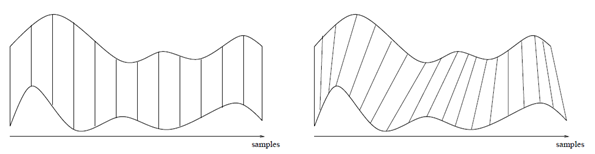
\includegraphics[width=1\textwidth]{./figures/dtw_dequence_demo}      
\caption{Sample-by-sample na\"{\i}ve alignment (left) versus an alignment performed using DTW (right) \cite{rath2003word}.}
\label{fig:dtw_dequence_demo}
\end{figure}

\iftoggle{edit-mode}{\hspace{0pt}\marginpar{Warping path Definition}}{}
\begin{definition}
Given two time series, $X = (x_1,x_2,...,x_n)$ and $Y = (y_1,y_2,...,y_m)$, the \emph{warping path} $W=(w_1,w_2,...,w_K)$ where ${w_k} = (i_k,j_k)$ is an alignment between the two sequences which satisfies the following conditions: 
\begin{enumerate}
\item Start and end point constraint: $w_1 = (1,1)$ and $w_k = (n,m)$. 
\item Local continuity constraint: ${w_{k + 1}} - {w_k} \in \left\{ {\left( {1,1} \right),\left( {1,0} \right),\left( {0,1} \right)} \right\}$
\end{enumerate}	 
The weight of a given warping path $W$ is defined as:
\begin{equation}
G(W) = \sum\limits_{k = 1}^{K} d(x_{i_k},y_{j_k} )
\end{equation}
where $d(x_{i_k},y_{j_k})$ is the distance between the points $x_{i_k}$ and $y_{j_k}$.
\label{def:warping_path}
\end{definition}

\iftoggle{edit-mode}{\hspace{0pt}\marginpar{DTW Definition}}{}
Equipped with the definition of a warping path, DTW is defined as follows:
\begin{equation}
DTW(X,Y)=\min\limits_{W} {G(W)}
\end{equation}
Namely, DTW returns the weight of the path which is associated with the optimal alignment.\\
Using a dynamic programming approach, DTW yields the optimal warping path by constructing the \emph{accumulated distance matrix} $D \in \mathds{R}^{m \times n}$. 
$D(i,j)$ is the minimum distance warping path that can be constructed from the two time series $X = \left( {{x_1},{x_2},...,{x_i}} \right)$ and $Y = \left( {{y_1},{y_2},...,{y_j}} \right)$.
The accumulated distance matrix is calculated as seen in Algorithm \ref{alg:adm_dtw}. \\
The value in $D(m,n)$ contains the minimum-distance warping path between $X$ and $Y$.
The optimal warping path $W$ is retrieved by backtracking the matrix $D$ from the point $D(m,n)$ to the point $D(1,1)$ following the greedy strategy of looking for the direction from which the current distance is taken \cite{senin2008dynamic}.
 
\begin{algorithm}
$D(1,1) = 0$\;
\For{$i\leftarrow 2$ \KwTo $n$}{
	$D(i,1) = d(x_i,y_1)$\;
}
\For{$i\leftarrow 2$ \KwTo $m$}{
	$D(1,j) = d(x_1,y_j)$\;
}
\For{$i\leftarrow 2$ \KwTo $n$}{
	\For{$j\leftarrow 2$ \KwTo $m$}{
		$D(i,j) = d(x_i,y_j) + \min {\left\{D(i,j - 1),D(i - 1,j),D(i - 1,j - 1)\right\}}$\;
	}
}
\caption{Accumulated distance matrix ($D$) construction}
\label{alg:adm_dtw}
\end{algorithm}

\iftoggle{edit-mode}{\hspace{0pt}\marginpar{stroke trajectories similarity measure using DTW}}{}
Handwritten strokes can be seen as temporal sequences in the planar space. 
In the on-line HWR, the exact temporal information is discarded in most cases by re-sampling the strokes to obtain equidistant sampling. 
However, unlike off-line HWR, the ordering information of the samples is kept. 
As such, DTW is an intuitive method for calculating the correspondence between two strokes. 
It have been proved to be relatively efficient and effective for shape matching of handwritten words. 
DTW was used in \cite{rath2003word, rath2003indexing, moghaddam2009application} to calculate the similarity between handwritten script in historical documents. 
Saabne has used DTW for key-word searching in \cite{saabni2011fast, saabni2008keyword}.


\iftoggle{edit-mode}{\hspace{0pt}\marginpar{DTW Speedup}}{}
The main drawback of DTW is its quadratic time and space complexity, i.e., $O(mn)$ where $m$ and $n$ are the time series lengths. 
Therefore, several speed-up methods have evolved \cite{salvador2007toward,rath2003word}.\textbf{Constraints enforcing}, i.e., limiting the amount of calculated cells in the accumulated distance matrix by imposing constrains on the calculation in the cells of the accumulated distance matrix, is a popular speed-up technique.
In some cases DTW tends to create an unrealistic correspondence between time-series features by aligning short features from one of the series to the long features on the second time series. 
To avoid this undesired phenomenon, constrains can be imposed on the possible correspondence between several consecutive points on the warping path. 
Two such constraints are the Sakoe-Chuba Band \cite{sakoe1978dynamic} and he Itakura parallelogram \cite{itakura1975minimum} as can be seen in Figure \ref{fig:dtw_dequence_demo}.
The greyed out area is the cells of the $D$ matrix that are filled by the DTW algorithm for each constraint. 
The warping path is looked for in the constraint window. 
The width of the window is specified by a parameter. 
Note that such constrains limit the amount of calculation needed for computing DTW, however, the speed-up factor is a constant and the DTW complexity remains quadratic. 
Furthermore, if the warping path is does not reside in the constraint window, it will not be found by DTW, therefore, such methods are usually used when the warping path is expected to be in the constrain window.


%\begin{compactitem}
%\item Constraints Enforcing: Limiting the amount of calculated cells in the accumulated distance matrix. 
%A more detailed explanation is given in the next paragraph.
%\item Data Abstraction: Speed-up using data abstraction is performed by running DTW on a reduced presentation of the data thus reducing the cell numbers that need to be computed. 
%The warp path is calculated on the reduced resolution matrix and mapped back to the original (full) cost matrix. 
%\emph{FastDTW} which was proposed in \cite{salvador2007toward} is an example of such approach.
%\item Lower Bounding: A lower-bounding is cheap and approximation of the DTW.
%It usually underestimates the actual cost determined by DTW. 
%It is used to avoid comparing series by DTW when the lower-bounding estimate indicates that the time series is worse match than the current best match \cite{rath2003word} 
%Lower bounding will be discussed in more details in Section \ref{subsec:lower_bounding}.
%\end{compactitem}

\iftoggle{edit-mode}{\hspace{0pt}\marginpar{How DTW is used in this work?}}{}
In this work, DTW is used for candidates re-scoring (described in chapter \ref{sec:candidates_scoring}). 
Actually, the $k$-NN are found among the entire dataset based on approximation of the EMD metric. 
Then, DTW is employed for attaching a more accurate similarity ranking between the query sample and its nearest neighbours.

\begin{figure}
\centering
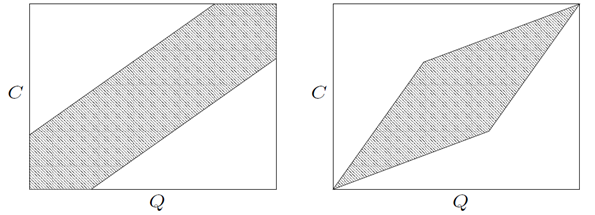
\includegraphics[width=0.7\textwidth]{./figures/dtw_sukoe_chuba}       
\caption{Cost matrix constraints: Sakoe-Chiba band (left) and the Itakura parallelogram (right).}
\label{fig:dtw_sukoe_chuba}
\end{figure}

%%%%%%%%%%%%%%%%%%%%%%%%%%%%%%%%%%%%%%%%%%%%%%%%%%%%%%%
\newpage{}
%%%%%%%%%%%%%%%%%%%%%%%%%%%%%%%%%%%%%%%%%%%%%%%%%%%%%%%

\section{Similarity Search}
\label{sec:similarity_search}
 
\iftoggle{edit-mode}{\hspace{0pt}\marginpar{Introduction}}{}
In Section \ref{sec:similarity_measures} we discussed the effectiveness aspect of measuring the perceptual notion of similarity between two objects.
However, even the most qualitative similarity measure technique is almost useless if for a given query object, the task of searching for similar objects in the database cannot be done efficiently.
Efficient similarity search usually requires the development of search methods that minimize the overall search costs.

\iftoggle{edit-mode}{\hspace{0pt}\marginpar{Similarity search query types}}{}
Similarity based search introduce two fundamental query types: \textbf{queries} and \textbf{k-NN queries} \cite{hetland2009basic}. 
Formal definitions of both query types are provided in Definitions \ref{def:range_query} and \ref{def:knn_query} and visualized in Figure \ref{fig:similarity_query_types}.
While range queries are argued to be fundamental, $k$-NN queries notably take a large volume in the literature.

\begin{definition}
Given a data space $\mathfrak{D}$, a distance function, $dist$, defined on $\mathfrak{D}$, a query object $q$ and a range parameter $r \geq 0$, the \textbf{range query} returns all the data objects in $\mathfrak{D}$ that are within distance $r$ from the query object $q$. 
Namely,
\begin{equation}
Range(q,r,\mathfrak{D},dist)=\{o \in \mathfrak{D} | dist(q,o) \leq r \}
\end{equation}
\label{def:range_query} 
\end{definition}

\begin{definition}
Given a data space $\mathfrak{D}$, a distance function, $dist$, defined on $\mathfrak{D}$, a query object $q$, the \textbf{k-nearest neighbours} (k-NN) query returns the $k$-closest objects in $\mathfrak{D}$ to the query object $q$. Formally,
\begin{equation}
k-NN(q,\mathfrak{D},dist)=\{A \subseteq \mathfrak{D} | \forall a \in A, b \in \mathfrak{D} \setminus A: dist(q,a) \leq dist(q,b) \wedge |A|=k \}
\end{equation}
\label{def:knn_query} 
\end{definition}

\begin{figure}[h!]
	\centering
        \fbox{\subfloat[]{
            \label{fig:range_query}
            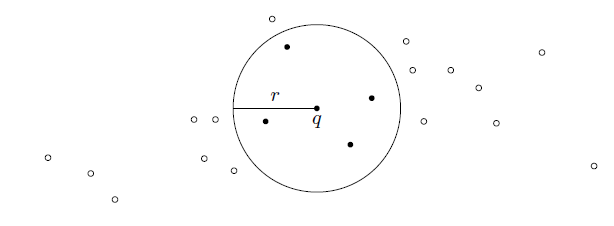
\includegraphics[width=0.4\textwidth]{./figures/range_query}
        }}
        \fbox{\subfloat[]{
           \label{fig:knn_query}
           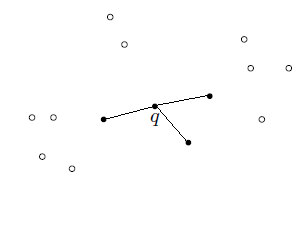
\includegraphics[width=0.4\textwidth]{./figures/knn_query}
        }}     
    \caption{Visualization of the \textbf{range} (\ref{fig:range_query}) and the \textbf{$k$-NN} (\ref{fig:knn_query}) queries in the two-dimensional Euclidean space.}
   \label{fig:similarity_query_types}
\end{figure}

\iftoggle{edit-mode}{\hspace{0pt}\marginpar{Problems - similarity search costs}}{}
The efficiency of a search method is defined as the time needed to evaluate a query. 
The query efficiency is affected mainly by two components; the \textbf{computation} cost and the \textbf{disk access time} (I/O) cost. 
The computation cost represents the effort spent in calculating the similarity measure function. 
The I/O cost is determined by the volume of data needed to be investigated to evaluate a query. Namely, the number of samples in the dataset that needs to be examined \cite{saabni2013efficient}.\\
Decreasing the computational cost can be obtained by using a cheap distance measure function which approximates, usually by providing a lower bound, the similarity between two given sample objects. 
The lower bound is used to filter out candidates with a similarity distance larger than a pre-set threshold. 
However, reducing the disk access cost can be attained only by discarding entire portions of the dataset which are assured to be distant enough from the given query object. 
Such techniques are called \emph{Metric Indexing} and will be discussed in Section \ref{sec:metric_indexing}.


\subsection{Lower Bounding}
\label{subsec:lower_bounding}
\iftoggle{edit-mode}{\hspace{0pt}\marginpar{Distance function approximation}}{}
In order to improve upon evaluating the distance function on every object in the dataset, we must somehow infer that an object $x$ can be included in, or excluded from, the search result without calculating the distance function $dist(q, x)$. One option to do so is by finding a cheap way of approximating the distance function. 
Although, both lower and upper bounding measures can be exploited to avoid running expensive calculation of the distance function $dist$, lower bounding appears to be more useful since it can be safely used to exclude far candidates, as described in Algorithm \ref{alg:lower_bound}. 
The more the approximation function $d$ is accurate, the less the actual distance function $dist$ will be invoked. However, there will normally be a trade-off between the approximation quality and the cost of computation \cite{hetland2009basic, keogh2005exact}.

\begin{algorithm}
$best\_so\_far = \infty$\;
\For{every object $x$ in database}{
	\If{$d(q,x) < best\_so\_far$}{
		$dist = d(q,x)$\;
	}
	\If{$dist < best\_so\_far$}{
		$best\_so\_far = dist$\;
		$nearest\_neighbor = x$\;
	}
}
\caption{A routine uses a lower bounding distance function, $d$, to speed-up the search for the nearest neighbour of the query object q in the database under the distance function $dist$.}
\label{alg:lower_bound}
\end{algorithm}

\subsection{Metric Embedding}
\label{subsec:metric_embedding}

\iftoggle{edit-mode}{\hspace{0pt}\marginpar{A different approach}}{}
The speed-up obtained by lower bounding is limited. 
An alternative approach is to embed the distance space imposed by the costly similarity measure, into a metric space equipped with a easy-to-compute distance function. 
Consequently, the calculation of distances between two elements in the embedded space would provide an inexpensive approximation to the actual distance between the two objects in the original space. 
A formal definition of the embedding is given in Definition \ref{def:embedding}.

\begin{definition}
Given metric spaces $(\mathfrak{D}, d)$ and $(\mathfrak{D}', d')$ a map $f : \mathfrak{D} \rightarrow \mathfrak{D}'$ is called an \textbf{embedding}.
\label{def:embedding}
\end{definition}

\iftoggle{edit-mode}{\hspace{0pt}\marginpar{Isometric embedding}}{}
The special case where $d(x, y) = d'(f(x), f(y))$ for all $x, y \in \mathfrak{D}$ is called \textbf{distance-preserving} or \textbf{isometric} embedding. However, isometric embeddings are very rarely beneficial, thus we allow the mapping to alter the distances in a restricted manner. The distortion of the embedding is defined in Definition \ref{def:embedding_distortion}.

\begin{definition}
Given two metrics $(\mathfrak{D}, d)$ and $(\mathfrak{D}',d')$ and a map $f : \mathfrak{D} \rightarrow \mathfrak{D}'$, the \textbf{contraction} of $f$ is the maximum factor by which distances are shrunk, i.e.,
\begin{equation}
\max_{x,y \in \mathfrak{D}} \frac{d(x,y)}{d'(f(x),f(y))}
\end{equation}
The \textbf{expansion} of $f$ is the maximum factor by which distances are stretched. Formally:
\begin{equation}
\max_{x,y \in \mathfrak{D}} \frac{d'(f(x),f(y))}{d(x,y)}
\end{equation}
and the \textbf{distortion} of $f$ is the product of the distortion and the expansion.
\label{def:embedding_distortion}
\end{definition}

\iftoggle{edit-mode}{\hspace{0pt}\marginpar{$L_p$ advantage and drawbacks}}{}
Using normed spaces (see Definitions \ref{def:norm}) such as the $L_p$ norm (see Definitions \ref{lp}) to solve the dissimilarity measure problem, allow using data structures that facilitate sub-linear $k$-NN retrieval.

\begin{definition}
Given a data space $\mathfrak{D}$, for any two data elements  $x,y \in \mathfrak{D}$, a \textbf{norm} $\|\cdot\|$ is defined as:
\begin{equation}
\|\cdot\|: \mathfrak{D} \longrightarrow \mathds{R}
\end{equation}
where the following conditions hold:
\begin{compactitem}
\item $\|x\|=0 \Leftrightarrow x=0$
\item $\|x-y\| \geq|\|x\|-\|y\||$
\item $\|\alpha x\|=|\alpha|\|x\|$
\end{compactitem}
the pair $\left(\mathfrak{D},\|\cdot\|\right)$ is called a \textbf{normed space}.
\label{def:norm}
\end{definition}


\begin{definition}
Given an vector space $V=\mathds{R}^N$ and $v=(v_1,v_2,...,v_N) \in V$, the $L_p$ norm is defined as:
\begin{equation}
\|v\|_p=\sqrt[p]{\sum\limits_{i=1}^N v_i^p}
\end{equation}
\label{lp}
\end{definition}
In this case we will denote this vector space as $L_p^N$ to emphasize the fact it is $N$ dimensional.

\subsection{Approximating EMD using Embedding}
\label{subsec:approximating_emd_using_embedding}

\iftoggle{edit-mode}{\hspace{0pt}\marginpar{Indyk and Thaper Embedding}}{}
Several approximation algorithms have been proposed to speed-up the computation of EMD. 
Indyk and Thaper \cite{indyk2003fast} proposed a technique for embedding the un-normed EMD metric into the $L_1$ space so that the EMD distance between the two objects is comparable to the Manhattan distance between the two points which represent the embedding of the two objects.  
Given two points sets $A$ and $B$, both of cardinality $N$ and containing points in $L_2^d$ space, the embedding given in \cite{indyk2003fast} is into the $L_1^d$ norm (i.e., the space of vectors in $\mathds{R}^d$ equipped with the Manhattan norm).
The general idea of the embedding is to compute and concatenate several weighted histograms of decreasing resolution for a given point set. 
Let us assume that the smallest distance between any two points is $1$, and $\Delta$ is the diameter of $C=A \bigcup B$. 
The embedding can be described as imposing hierarchy of grids $G_i$ having side length $2^i$ on the space $\mathds{R}^d$, where $-1 \leq i \leq \log \Delta$. 
It is required that each grid $G_{i}$ be a refinement of the grid $G_{i+1}$. 
Each grid is translated by a vector chosen randomly from $[0, \Delta]^d$. 
For each grid $G_i$, the vector $v_i(A)$ contains a single coordinate per cell that contains the number of points in the corresponding cell. 
In fact, for every $i$, $v_i(A)$ forms a histogram of A. 
The embedding, denoted as $f_{EMD}(A)$, is then defined as the concatenated vector of the $v_i$'s, scaled by the grid side lengths. 
Formally,
\begin{equation}
f_{EMD}(A) = [v_{-1}(A)/2, v_0(A), 2v_1(A), 4v_2(A),..., 2^iv_i(A),...]
\end{equation} 
Figure \ref{fig:emd_embedding} provides a visual demonstration of the embedding.
Approximating the EMD distance between the set $A$ and $B$ is then done by calculating the Manhattan distance between the two corresponding embedding vectors, i.e.,
\begin{equation}
EMD_{approx.}=|f_{EMD}(A) - f_{EMD}(B)|
\end{equation}  

\begin{figure}
\centering
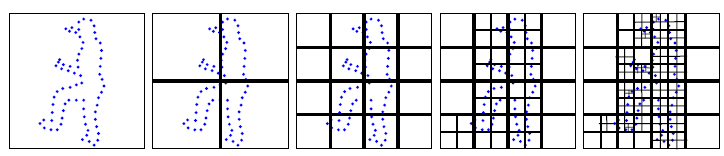
\includegraphics[width=0.7\textwidth]{./figures/emd_embedding}       
\caption{Embedding of a shape contour \cite{grauman2004fast}.}
\label{fig:emd_embedding}
\end{figure}

\iftoggle{edit-mode}{\hspace{0pt}\marginpar{Performance}}{} 
The time complexity of the embedding is $O(Nd \log{\Delta})$. 
The distortion of the embedding has an upper bound of $O(\log \Delta)$. 
A detailed proof is provided in \cite{indyk2003fast}. 
However, the proved theoretical distortion can only provide a weak practical instrument. 
Nevertheless, experimental validation performed on a dataset of $20,000$ objects showed a $(1+\epsilon)-approximate$ nearest neighbour, with $\epsilon < 20\%$ that was achieved by the embedding compared to the exact EMD. 
Grauman and Darrel \cite{grauman2004fast} have used this embedding for contour matching and experimentally validated the quality of retrieval. 
They have found that the accuracy reduction is less than $10\%$ compared to the exact EMD.

\subsubsection{EMD Embedding using the Wavelet Coefficients Domain}
%compare this embeddign technique to the previous one.
%How it is done?
%Is it faster to calculate?
%Is the retrieval more accurate (empirically) than the $L_1-EMD$ embedding?
%Are the bounds are more strict? 
%printf('%s','5ara 3leek ba7ebak') //by Reema Salma Darawshe

\iftoggle{edit-mode}{\hspace{0pt}\marginpar{Wavelet embedding}}{}
In a subsequent work done by Shirdhonkar and Jacobs \cite{shirdhonkar2008approximate}, the authors proposed a linear time method for approximating the EMD between two low dimensional histograms using the weighted wavelet coefficients of the difference histogram. 
It is done by calculating the $L_1$ norm of the coefficients vector of the embedding as given in Equation \ref{eq:emd_embedding}.

\begin{equation}
d(p)_{wemd}= \sum\limits_{\lambda} 2^{-j(1+n/2)}|p_{\lambda}|
\label{eq:emd_embedding}
\end{equation}
where $p$ is the n-dimensional difference histogram and $p_{\lambda}$ is the wavelet transform coefficients. 
The index $\lambda$ includes both shifts and the scale j.
They proved that the ratio of the approximation and the real EMD is bounded by constants. 

\iftoggle{edit-mode}{\hspace{0pt}\marginpar{Intuitive explanation}}{}
Intuitively, the wavelet transform splits up the difference histogram according to scale and location where each coefficient represents the solution to the EMD subproblem. 
For a single wavelet, the mass to be moved is proportional to the volume of $|\psi_j(x)|$, i.e., to $2^{-jn/2}$ and the distance to be travelled is proportional to the span of the wavelet, i.e $2^{-j}$. 
The sum of all distances is an approximation to EMD, as formally defined in Equation \ref{eq:emd_embedding}. 
This can be viewed similar to the way packages are shipped over large distances. 
The route is broken into several pieces which are large and small distances. 
Packages from nearby places are merged at the end of the short distance route piece to travel together. 
Then another merge is done of packages from the entire country to be shipped together to the destination country. 
The sum of the distances travelled is an approximation to the actual distance. 
See Figure \ref{fig:emd_wavelet}.

\begin{figure}
\centering
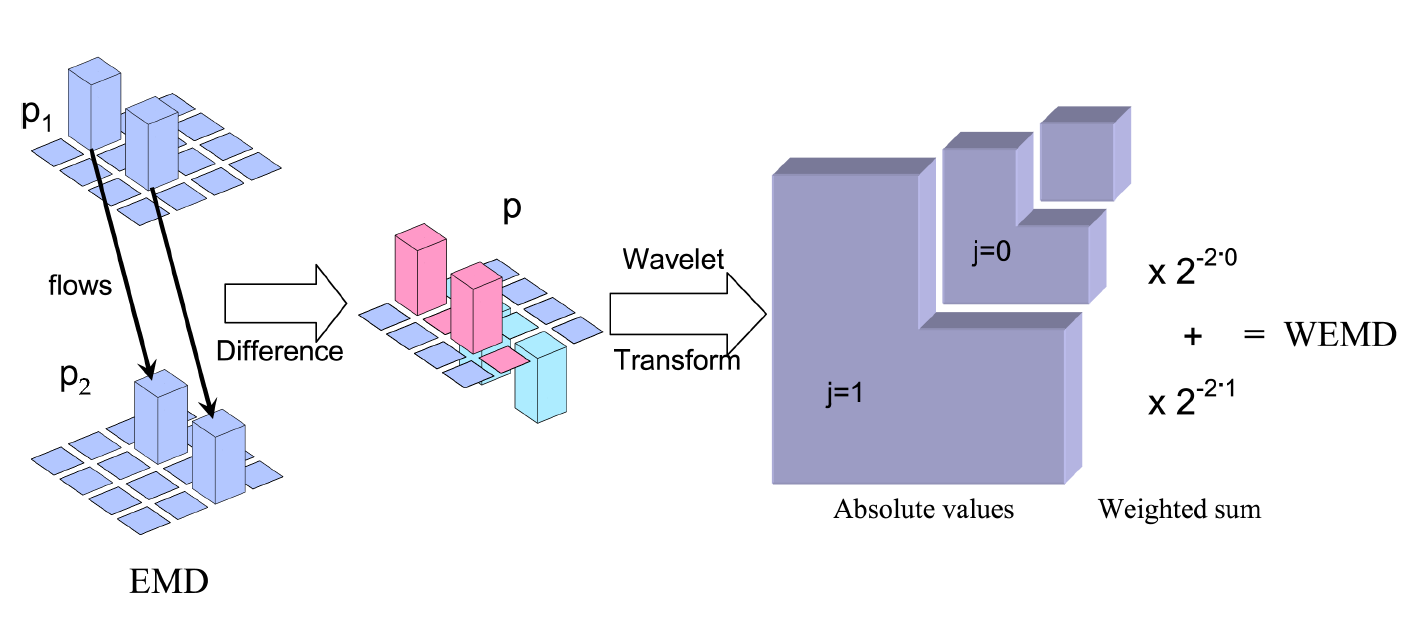
\includegraphics[width=1\textwidth]{./figures/emd_wavelet}       
\caption{EMD embedding using the wavelet domain \cite{shirdhonkar2008approximate}.}
\label{fig:emd_wavelet} 
\end{figure}

\iftoggle{edit-mode}{\hspace{0pt}\marginpar{Embedding the histograms rather than the difference histogram}}{}
However, in our application, where the histogram descriptors are to be stored rather than the difference histogram, the computation of EMD can be partitioned into two parts. 
First the histograms are converted into the wavelet domain and their coefficients are scaled according to Equation \ref{eq:emd_embedding}. 
Computing the EMD distance is done by calculating the Manhattan distance between the scaled coefficients of the corresponding histograms.

\iftoggle{edit-mode}{\hspace{0pt}\marginpar{shirdhonkar - theoretical and empirical bounds}}{}
Shirdhonkar and Jacobs provided both theoretical and experimental bounds. 
The theoretical approximation is based on Theorem 2 in \cite{shirdhonkar2008approximate}. 
Using a large dataset, they were able to experimentally establish that the proposed approximation follows the true EMD closely, and can be alternatively used without any significant difference in performance. 
The wavelet EMD metric can be computed in $O\left( N \right)$ time complexity. 

\iftoggle{edit-mode}{\hspace{0pt}\marginpar{Performance - Indyk vs. shirdhonkar}}{}
Empirically, the normalized RMS error obtained by using the wavelet embedding was between in 13\% and 20\% compared to the embedding proposed by Indyk and Thaper which achieved 43\% in the same experiment. 
In addition, the wavelet embedding surpassed the Indyk and Thaper embedding in time performance.
Note that the embedding process requires histograms, thus the vectors in the feature space need to be normalized before using this method.

Shirdhonkar and Jacobs tested few wavelets and showed that the \textbf{Coif-lets} of order 3 and the \textbf{Symmetric Daubechies} wavelets of order 5 have lowest error rates. 
We evaluated several wavelets, including the \textbf{Haar} wavelet, the \textbf{Coif-let} of order 1, the \textbf{Coif-let} of order 2 and the \textbf{Symlets} of order 5 wavelets.
The \textbf{Haar} wavelet achieved the best classification results.
Embedding the SC feature vectors has produces sparse vectors in $\mathds{R}^{2422}$.

 
%%%%%%%%%%%%%%%%%%%%%%%%%%%%%%%%%%%%%%%%%%%%%%%%%%%%%%%
\newpage{}
%%%%%%%%%%%%%%%%%%%%%%%%%%%%%%%%%%%%%%%%%%%%%%%%%%%%%%%

\section{Dimensionality Reduction}
\label{sec:dr}

\iftoggle{edit-mode}{\hspace{0pt}\marginpar{What is DR and what techniques are there?}}{}
\emph{Dimensionality Reduction} is a process of reducing the number of variables taken into consideration in the learning and classification of data. 
It is a fundamental process in machine learning since it facilitates classification, efficient storing and visualization of data. 
The undesired properties of high-dimensional data present many mathematical challenges and practical complications \cite{van2009dimensionality}. 
First, analysis of high-dimensional data generally requires a large amount of memory and computation power, which may be impractical for on-line classification systems and obstructive in other applications. 
In particular, several nearest neighbours retrieval methods such as $k$-d tree are ineffective when the dimensionality of the data is high.
Second, when the data dimensionality is high the classification algorithm is more likely to over-fit the training sample and generalizes poorly to new samples \cite{aida2009word}.
The high dimensional data phenomenon is widespread in data analysis and was given the name \emph{the curse of dimensionality}. 

\iftoggle{edit-mode}{\hspace{0pt}\marginpar{data Intrinsic dimensionality}}{}
Ideally, the dimensionality of the reduced representation should correspond to the intrinsic dimensionality of the data \cite{van2009dimensionality}.
The intrinsic dimensionality of data is the minimum number of properties needed to account for in the observed data. 
The belief underlying the existence of a compact representation of the external world data is based on the observation that the human brain can instantaneously and precisely recognize an observed apple, smile or a handwritten letter within a short route of neural computations. 
However, a digital representations of these images may consist of hundreds or thousands of pixels. 
Clearly, there are much more compact representations of images, sounds, and even text than their native digital formats. 
Several recently proposed dimensionality reduction techniques are based on the intuition that data lies on or near a complex low-dimensional manifold that is embedded in the high-dimensional space.

\iftoggle{edit-mode}{\hspace{0pt}\marginpar{The curse of dimensionality}}{}
The curse of dimensionality can arise in different stages of the learning and classification process; 1. the dimensionality of the raw data may be high, such as videos an images; 2. features calculated on the data may be impractically large; 3. other manipulations performed on the data may produce highly dimensional vectors.

\iftoggle{edit-mode}{\hspace{0pt}\marginpar{Why do we need DR?}}{}
The highly dimensional sparse vectors produced by the EMD embedding and the sensitivity of the $k$-d tree to high dimensional required us to add a dimensionality reduction stage.
The wish to employ $k$-d trees, which is very sensitive to high dimensional data, was the main reason for using dimensionality reduction. 
An alternative was to use a $k$-NN data-structure that performs well with high dimensional data such as \emph{Locality Sensitive Hashing} (LSH) \cite{gionis1999similarity}. 
However, it would be less accurate since LSH is an approximate NN search method, unlike $k$-d tree which can be used to find the exact $k$-NN samples.

\iftoggle{edit-mode}{\hspace{0pt}\marginpar{Mathematical Definition}}{}
Mathematically, given $p$-dimensional variable $x \in \mathds{R}^p$, the dimensionality reduction process finds a lower dimensional representation $s \in \mathds{R}^k$ with $k \ll p$ which preserves the content of the original data under a given criterion. 
The reduced dimensionality $k$ is chosen to be as small as possible, but yet sufficiently large to guarantee that the output vector $s$ provide a faithful representation of the input vector $x$. 
Dimensionality reduction techniques can be classified into linear and non-linear. \\
Linear dimensionality reduction is based on a linear projection of the data, assuming the data resides close to a lower dimensional linear subspace. 
Namely, each of the components in the vector $s$ is a linear combination of the components in the vector $x$, formally:
\begin{equation}
s=Wx
\end{equation}
where $W_{k \times p}$ is the linear transformation.

\iftoggle{edit-mode}{\hspace{0pt}\marginpar{Non-Linear DR}}{}
In some cases, linear dimensionality reduction techniques perform poorly and a intensified approach is required to provide the mapping from the high dimensional space to the low dimensional space. 
In such cases, non-linear techniques are used. 
Yet, the drawback of such techniques is concealed in its generality which may cause over-fitting on the sample set and not really capturing the true underlying coordinate system. 
Commonly used non-linear technique include \emph{Kernel PCA}, \emph{Isometric Feature Mapping} (ISOMAP) and \emph{Locally Linear Embedding} (LLE).

\iftoggle{edit-mode}{\hspace{0pt}\marginpar{What DR we use?}}{}
In this thesis we have chosen to work only with linear dimensionality reduction techniques. 
\emph{Principle Component Analysis} (PCA) and \emph{Linear Discriminant Analysis} (LDA) were applied sequentially in order to obtain linearly discriminative information efficiently.

\iftoggle{edit-mode}{\hspace{0pt}\marginpar{PCA}}{}
PCA is a popular linear dimensionality reduction technique proposed by Karl Pearson \cite{pearson1901principal} in 1901.
It is "unsupervised" in the sense that the labelling of the data do not effect the determination of the transformation function. 
PCA produces an orthogonal linear transformation that projects the data into a new coordinate system such that the greatest variance by any projection of the data comes to lie on the first coordinate (called the first principal component), the second greatest variance on the second coordinate (called the second principal component) and so on, as seen in Figure \ref{fig:pca_demo}. 
The principal components as a whole form an orthogonal basis. 
Given a multivariate dataset visualized as a set of coordinates in a high-dimensional data space, PCA obtains the "shadow" of that dataset when viewed from its most informative viewpoints by projecting the dataset into a lower-dimensional space formed by the first few principal components.

\begin{figure}
\centering
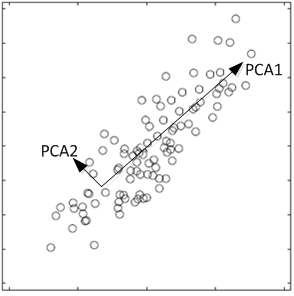
\includegraphics[width=0.4\textwidth]{./figures/pca_demo}       
\caption{The first and second principal component of the data elements, labelled as \emph{PCA1} and \emph{PCA2 }respectively.}
\label{fig:pca_demo}
\end{figure}

\iftoggle{edit-mode}{\hspace{0pt}\marginpar{PCA formulation}}{}
In computational terms the principal components are found by calculating the eigenvectors and eigenvalues of the data covariance matrix. 
This process is equivalent to finding the axis system in which the co-variance matrix is diagonal. 
The eigenvector with the largest eigenvalue is the direction of greatest variation. 
The eigenvalues represent the distribution of the source data energy among each of the eigenvectors, where the eigenvectors form a basis for the data. 
The representation content $g$ for the $j^{th}$ eigenvector is the sum of the energy content across all of the eigenvalues $\lambda_k$ from $1$ to $j$ :
\begin{equation}
g[j]=\sum_{k=1}^{j}\lambda_k 
\end{equation}
for $1 \leq j \leq d$ and $d$ denotes the dimensionality of the original data. 
The \emph{data preservation rate} value, $E$, is calculated as seen in Equation \ref{eq:dr_energy}. 
\begin{equation}
E[\ell] = \frac{g[\ell]}{g[d]}
\label{eq:dr_energy} 
\end{equation} 
The goal is to find the smallest possible $\ell$ that achieves $E[\ell]$ value which rise above a pre-set threshold, usually larger than $0.9$. 
This dimensionality estimation technique is known as the \emph{eigenvalue-based dimensionality estimator}. 

\iftoggle{edit-mode}{\hspace{0pt}\marginpar{LDA}}{}
The major drawback of PCA is that it is an unsupervised technique and as such does not use label information of the data. 
The following example, given by Welling in \cite{welling2005fisher}, demonstrates the problem in using PCA. 
In Figure \ref{fig:cigarettes_data}, we see two parallel cigar like clusters. 
The variance of the entire sample set, disregarding the labels, is in the direction of the cigars. 
Projecting the sample set on the principal component would terribly mix the samples. 
Clearly, a better projection would be orthogonal to the cigars, namely in the direction of least overall variance, which perfectly separate the two classes.
LDA, a descendant of the original Fisher-LDA \cite{fisher1936use}, overcomes this problem. 
Unlike PCA, LDA is a supervised technique. 
It attempts to model the difference between classes of data based on the samples labelling. 
In this method, variability among the feature vectors of the same class is minimized and the variability among the feature vectors of different classes is maximized. 
LDA performs dimensionality reduction while preserving as much of the class discriminatory information as possible. 
A brief tutorial on LDA is given in \cite{balakrishnama1998linear}. 
Without going into the math, in order to find a good projection vector, we need to define a measure of separation between the projections. 
The solution proposed by Fisher is to maximize a function that represents the difference between the means, normalized by a measure of the within-class scatter. 
LDA has three main drawbacks; the first is that it assumes that the data resides in $L_2$; second, LDA assumes that the distribution of the samples in each class is Gaussian which is not necessarily true; third, it is much slower to calculate compared to PCA.
Note that even though LDA is preferred in many application, it does not always outperform PCA.  


\begin{figure}
	\centering
        \subfloat[]{
            \label{fig:ldapca}
            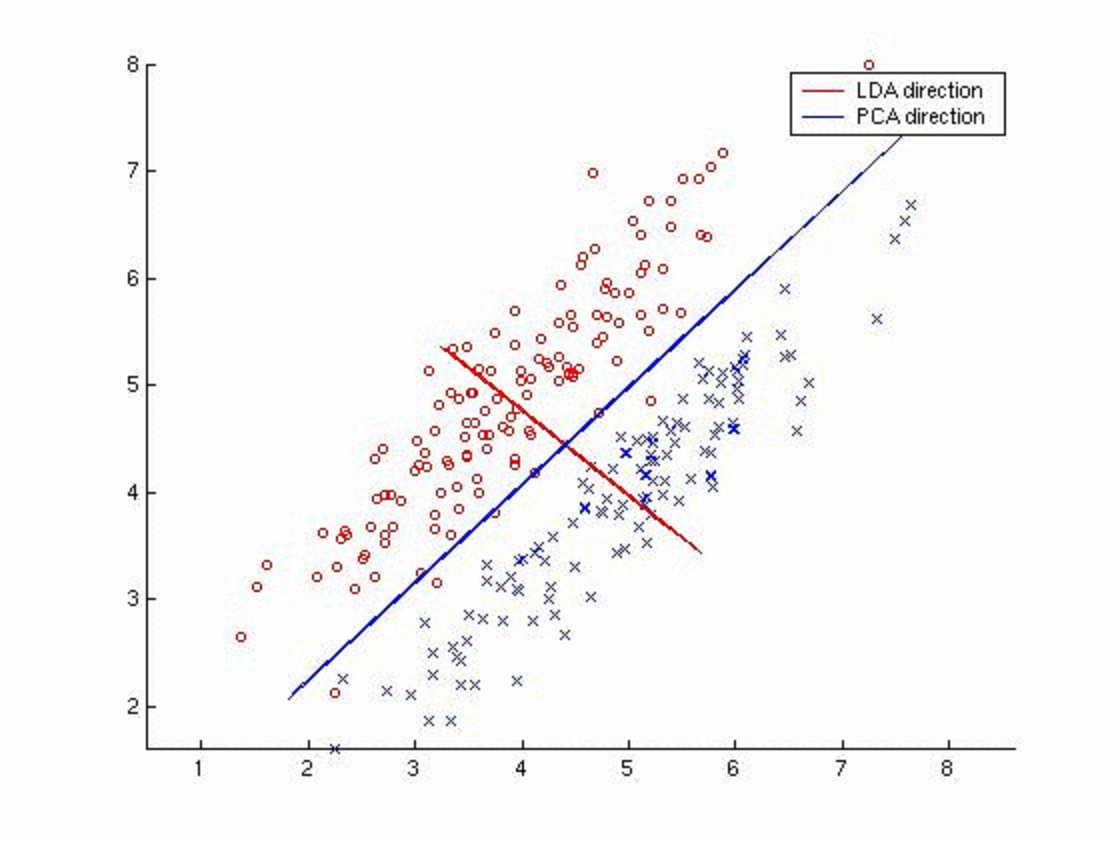
\includegraphics[width=0.5\textwidth]{./figures/ldapca}
        }
        \subfloat[]{
           \label{fig:ldapca_graph}
           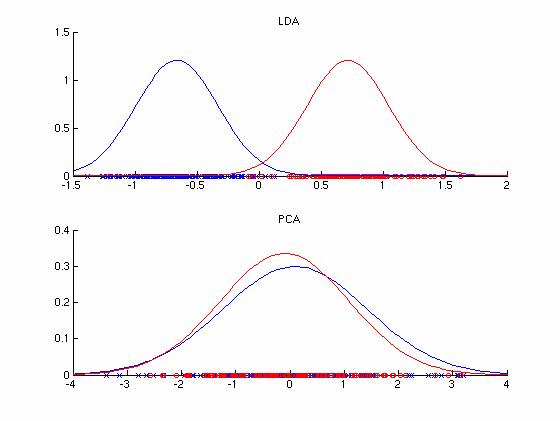
\includegraphics[width=0.5\textwidth]{./figures/ldapca_graph}
        }
    \caption{A cigarettes like spread of data samples is shown in \ref{fig:ldapca}. 
    The samples projection and distribution in the PCA and LDA projection directions is compared in \ref{fig:ldapca}}
   \label{fig:cigarettes_data}
\end{figure}


\iftoggle{edit-mode}{\hspace{0pt}\marginpar{When to perform the DR?}}{}
Grauman et al. in \cite{grauman2004fast} used PCA to find a low-dimensional subspace based on a large sample of the SC histogram. 
PCA yields the set of bases that define a low-dimensional "shape context manifold". 
Only then the approximate EMD embedding is performed. 
However, we have chosen to perform the stages in a different order. 
First, approximate EMD embedding is performed on the feature vectors, and only then, dimensionality reduction procedure is applied on the sparse embedded vectors. 
The reason we have chosen to perform the stages in this order is that if we were to apply the order suggested by Grauman, we would still result in a large sparse vectors constructed by the embedding process.
  
\iftoggle{edit-mode}{\hspace{0pt}\marginpar{Usage of PCA in the $L_1$ space.}}{}
PCA and LDA are basically defined over $L_2$ while the embedding into the wavelet coefficients domain was proved to approximate EMD in $L_1$. 
Nevertheless, we decided to use the basic form of PCA, given that $L_2$ estimates $L_1$ fairly well.

\iftoggle{edit-mode}{\hspace{0pt}\marginpar{Implementation: PCA}}{}
In order to exploit the strengthens of both PCA (efficiency) and LDA (discrimination power) we've used the dimensionality reduction process outlined as follows. 
The data samples are projected to a subspace $S_1$ using PCA and then to subspace $S_2$ using LDA. 
In the PCA stage, the target dimensionality, is the minimal to achieve data preservation rate of 99\%. 
As mentioned before, the dimensionality of the embedded vectors was $2422$. 
The reason we adopted such high preservation rate is that it was enough to secure a major dimensionality reduction. 
As seen in table \ref{table:dr_dimensions_results}, the dimensionality was reduced in two orders of magnitude by PCA.

\begin{table}
\centering
\caption{The dimensionality of the four datasets after applying PCA and PCA+LDA.}
\begin{tabular}{ c c c c }
\toprule
\textbf{Letter position} & \textbf{Number of samples} & \textbf{PCA} & \textbf{PCA+LDA} \\
\midrule                 
  Ini & 1405 & 48 & 9 \\ 
  Mid & 1196 & 52 & 10 \\ 
  Fin & 1629 & 44 & 9 \\ 
  Iso & 1372 & 39 & 8 \\ 
  \bottomrule
\end{tabular}
\label{table:dr_dimensions_results} 
\end{table}

\iftoggle{edit-mode}{\hspace{0pt}\marginpar{Implementation: Clustering and LDA}}{}
Applying LDA directly on the resulted data would have achieved poorer results due to the fact that almost all letters in the Arabic writing system have several shapes, relatively different, which are commonly used. 
Since LDA regards the labelling of the data samples, trying to group different perceptual shapes in a single class would impinge the dimensionality reduction process. 
In order to overcome this obstacle, we have done the following preprocessing steps: each class, namely the tuple $(letter, position)$, was clustered into four clusters using $L_1$-k-medoids algorithm. 
Each cluster received a unique class label. 
This new artificially labelled data was given as input to the LDA.

\iftoggle{edit-mode}{\hspace{0pt}\marginpar{LDA target dimensionality}}{}
Determining the target dimensionality of the LDA stage was done using the \emph{Maximum Likelihood Estimation} (MLE) method described in \cite{levina2004maximum}.
MLE belongs to a family of dimensionality estimation methods called \emph{Intrinsic dimensionality estimation}.
Intrinsic dimensionality estimation techniques are based on the observation that for a given data point $x_i$ the number of sample points covered by a hypersphere around the data point with radius $r$ grows proportional to $r^d$; where $d$ is the intrinsic dimensionality of the data manifold around that data sample.  
The function that estimates this relation for a given data point $x_i$ is named \emph{local estimator}.
The estimated intrinsic dimensionality $\hat{d}$ of the dataset is then calculated by averaging over the local estimators of the entire sample set \cite{van2007introduction}.

\iftoggle{edit-mode}{\hspace{0pt}\marginpar{The DR package}}{}
The dimensionality reduction stage was implemented using the \textbf{Matlab Toolbox for Dimensionality Reduction} package described in \cite{van2007introduction}.

%%%%%%%%%%%%%%%%%%%%%%%%%%%%%%%%%%%%%%%%%%%%%%%%%%%%%%%
\newpage{}
%%%%%%%%%%%%%%%%%%%%%%%%%%%%%%%%%%%%%%%%%%%%%%%%%%%%%%%


\section{Metric Indexing}
\label{sec:metric_indexing}

\iftoggle{edit-mode}{\hspace{0pt}\marginpar{Motivation}}{}
Distance function approximation techniques alone cannot avoid linear scan of the entire dataset when searching for the $k$-NN of a query object. 
Efficient data retrieval in a metric dataset requires building a \emph{metric index}.
The main goal of indexing methods is to enable efficient searching, either asymptotically or simply in real wall-clock time. 
The time cost involved in building the index is amortized over the series of queries, and is usually ignored when considering search cost, and the fact that in most cases it is an off-line process \cite{hetland2009basic}.

\iftoggle{edit-mode}{\hspace{0pt}\marginpar{Introduction}}{}
Indexing techniques partition the dataset into equivalence classes in a way that each equivalence class contains objects that are sufficiently close to each other. 
However, this does not assure that close objects will always be contained in the same equivalence class. 
Each class is bounded by a hypersphere covering all the objects in the equivalence class. Consequently, at query time the index is efficiently searched to locate the equivalence classes which cover the areas where the closest objects may be contained. 
These classes are then exhaustively checked for the relevant objects.
This allows discarding classes that surely does not contain relevant objects. 
In order for the metric indexing to work correctly and efficiently, the distance function is required to satisfy the triangle equality.
 
\iftoggle{edit-mode}{\hspace{0pt}\marginpar{Exact vs. Approximate Indexing}}{}
Metric indexing techniques are split into two types: exact and approximate. 
Exact techniques are guaranteed to return the same result as  scanning the entire database. 
Approximate indexing methods return good matches, but not necessarily the best matches. 
Exact methods do not allow false positives or false negatives, i.e., all of the relevant objects are required to be returned in the query result, and only them. 
However, the approximate methods relax this strong requirement so that a small number of false negatives is acceptable \cite{keogh2005exact}. 
Many methods were proposed to solve the exact $k$-NN problem that are significantly better than a brute-force computation over the entire database. 
However, computing the approximate nearest neighbours, can achieve significantly faster retrieval with a relatively small actual error. 
Approximate nearest neighbours techniques also allow the user to specify a maximum approximation error bound, thus enabling the user to control the trade-off between accuracy and running time.

\begin{figure}
\centering
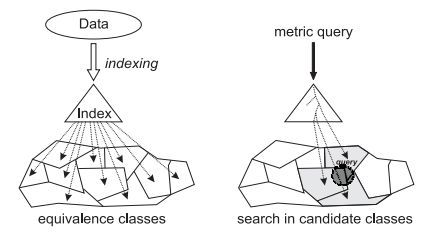
\includegraphics[width=0.7\textwidth]{./figures/indexing}       
\caption{Metric indexing and query.}
\label{fig:indexing}
\end{figure}

\iftoggle{edit-mode}{\hspace{0pt}\marginpar{Examples of Exact and Approximate Indexing}}{}
Approximate nearest neighbours methods such as $k$-d trees and LSH have been successfully applied on a variety of fast similarity retrieval problems.
The key assumption in these procedures is that the objects in the dataset lie in a metric space, i.e., the space satisfies the triangle equality; an assumption which may not be valid for many similarity measure techniques.
The $k$-d tree even requires a stronger requirement of $L_p$ space. 

\iftoggle{edit-mode}{\hspace{0pt}\marginpar{This work}}{}
While the advantage of LSH is that it performs better than $k$-d tree in high dimensional spaces, $k$-d tree can be used both as an exact and approximate $k$-NN technique. 
In this work, we have chosen to work with $k$-d tree since we could obtain, after applying the dimensionality reduction stage, a low dimensional data space.
In addition, the sensitivity of the segmentation process requires high classification accuracy.

%%%%%%%%%%%%%%%%%%%%%%%%%%%%%%%%%%%%%%%%%%%%%%%%%%%%%%%
\subsubsection{$k$-d tree}

\iftoggle{edit-mode}{\hspace{0pt}\hspace{0pt}\marginpar{A short introduction to $k$-d tree}}{} 
The $k$-d tree is an efficient data structure for storing a finite set of points from a $k$-dimensional space, proposed by Bentley in \cite{bentley1975multidimensional}. 
It aims at solving the $k$-NN problem in a large set of multi-dimensional points by first building a data structure based on the set of reference points. 

\iftoggle{edit-mode}{\hspace{0pt}\marginpar{How it works, how the data is saved and extracted}}{} 
The $k$-d tree is constructed as follows. 
Every point is either a branch node or contained in a leaf node. 
Every branch node in the tree is associated with one of the $k$-dimensions and can be though of an hyperplane that divides the space into two half spaces in that dimension. 
Points to the left of this hyperplane are represented by the left sub-tree of that node and points to the right of the hyperplane are represented by the right sub-tree, see Figure \ref{fig:kd_tree}. 
A desired property of the partition is to be as equal as possible. 
The selection of the pivot point (i.e,  the point that function as a branch node) in every level has a great impact on the balance of the tree. 
The most common way is to find the medial point of a number of points in the sub-tree. 
The number of points in a leaf node is also customizable and is mostly affected by the cardinality of the points in the database and the typical $k$, which is a predefined in many applications.

\begin{figure}
\centering
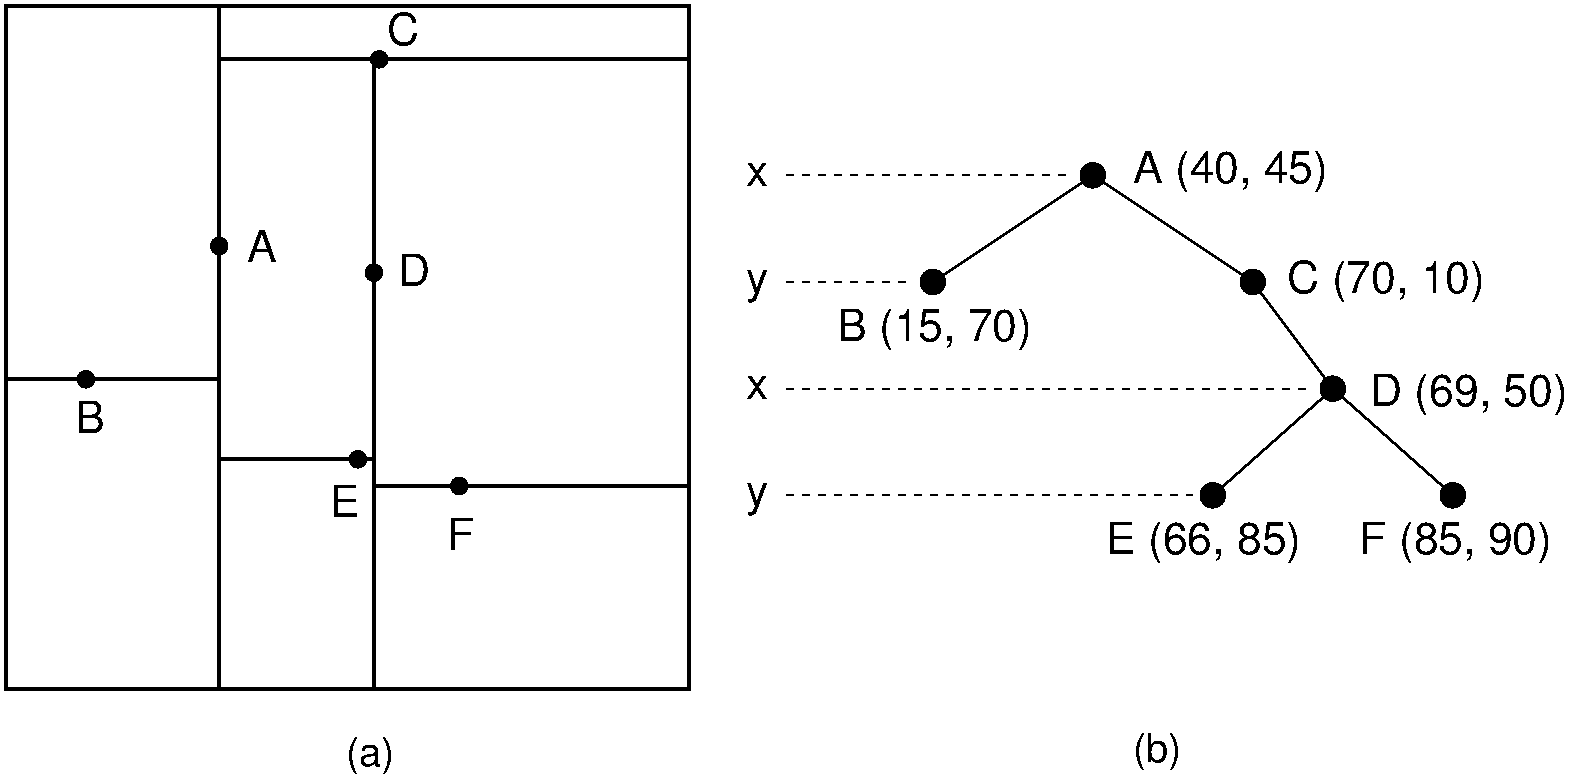
\includegraphics[width=0.8\textwidth]{./figures/kd_tree}       
\caption{Example of a $k$-d tree. (a) - The $k$-d tree decomposition of a region containing six data points. (b) - The $k$-d tree representation for (a).}
\label{fig:kd_tree}
\end{figure}

\iftoggle{edit-mode}{\hspace{0pt}\marginpar{How the NN are found?}}{}
The approximation of the $k$-NN in a $k$-d tree is done by initially finding the leaf node that represents the equivalence class that the query point belongs to. 
Although it is probable that the $k$-NN are all contained in a single leaf node, it is not necessarily the case. 
Adjacent leafs may be examined by recursively explore the other child nodes and look for the exact $k$-NN. 
 
\iftoggle{edit-mode}{\hspace{0pt}\marginpar{Expected time complexity}}{}
The construction time of the $k$-d tree is O($k N \log N$), where $k$ is the dimensionality of the data space and $N$ is the cardinality of the dataset. 
We can afford this high complexity of the construction since the this process is done off-line, and theoretically will be executed mostly several times. 
Therefore, this tax pays off when it comes to the enhancement we achieve in the k-$NN$ query evaluation. 
While the worst case scenario, the running time of $k$-NN is $O(N^{d^2})$, the amortized running time is $O(\log N)$.

\iftoggle{edit-mode}{\hspace{0pt}\marginpar{The Matlab library}}{} 
Our system uses a built-in Matlab implementation for $k$-d tree which is available in the statistical toolbox and introduced in Matlab R2013B. 
The library allows configuring the distance function (Euclidean, Manhattan, Mankowski, etc...) and the size of the leaf node. 
The library provides an implementation for the exact version of $k$-d tree.

%%%%%%%%%%%%%%%%%%%%%%%%%%%%%%%%%%%%%%%%%%%%%%%%%%%%%%%
\newpage{}
%%%%%%%%%%%%%%%%%%%%%%%%%%%%%%%%%%%%%%%%%%%%%%%%%%%%%%%

\section{Candidates Re-scoring}
\label{sec:candidates_scoring}
\iftoggle{edit-mode}{\hspace{0pt}\marginpar{The need for a re-scoring}}{} 
Given an unlabelled sequence $q$, the $k$-NN classifier, using the Manhattan distance, returns a set of $k$ potential letter candidates from the sample set and their scoring, i.e., the perceptual distance between the candidate and $q$.
As mentioned in Section \ref{def:embedding}, the Manhattan distance in the wavelets coefficients domain approximate the EMD distance between objects. 
However, in implementations that require exact scoring of the candidates, the approximated EMD distance may not be sufficient and an additional scoring stage should be employed to obtain a more accurate similarity measure between the query object and the candidates.
Nevertheless, as explained in Section \ref{sec:similarity_measures}, in most cases such similarity measure techniques are computationally expensive and can be applied only on a short list of candidates rather than on the entire sample set.   

\iftoggle{edit-mode}{\hspace{0pt}\marginpar{How re-scoring is done here}}{} 
In this work, re-scoring of the candidates is done by calculating the DTW distance between the preprocessed version of the query sequence and the candidates.
The constrained version of DTW using the Sakoe-Chuba Band \cite{sakoe1978dynamic} demonstrated better results than the unconstrained version of DTW.
$k$, the number of candidates returned by the $k$-d tree, is set to 10.
As we will see in the results sections, the re-scoring stage significantly affects the classification performance, in terms of accuracy and response time.\\
In order to measure the re-scoring effectiveness, in Section \ref{sec:classification_results} we compare between the classifier results when including and when avoiding the re-scoring stage.

%%%%%%%%%%%%%%%%%%%%%%%%%%%%%%%%%%%%%%%%%%%%%%%%%%%%%%%
\newpage{}
%%%%%%%%%%%%%%%%%%%%%%%%%%%%%%%%%%%%%%%%%%%%%%%%%%%%%%%

\section{Experimental Results}
\label{sec:classification_results}

\subsection{Classification Quality Measures}
\iftoggle{edit-mode}{\hspace{0pt}\marginpar{Classification types}}{}
There are three commonly used classification quality measurements for assessing the performance of a classification algorithm: \emph{Accuracy}, \emph{Precision} and \emph{Recall}.
In binary classification, each sample belongs to one of two classes, the positive class or the negative class.
A \emph{true positive} ($tp$) instance is an actual positive sample classified correctly as positive by the classification system.
Similarly, a \emph{true negative} ($tn$) instance is the case of a negative sample classified correctly as negative.  
Wrong classification of samples are of two types: a positive sample mistakenly classified as negative, named \emph{false positive} ($fp$), and the case of a negative sample classified as belonging to the positive class, i.e.,  \emph{false negative} ($fn$). 

\iftoggle{edit-mode}{\hspace{0pt}\marginpar{Classification quality measurements - binary}}{}
The \emph{Accuracy} is the fraction of the points in the sample set that were classified correctly. 
Formally,
\begin{equation}
\text{Accuracy}=\frac{tp+tn}{tp+fp+tn+fn}
\label{eq:accuracy}
\end{equation}
\emph{Precision} is the fraction of true positive among all the instances classified as positive. Namely,
\begin{equation}
\text{Precision}=\frac{tp}{tp+fp}
\label{eq:precision}
\end{equation}
The measure \emph{Recall} is the fraction of instances correctly classified as positive among all the positive samples, calculated as described in Equation \ref{eq:recall}.
\begin{equation}
\text{Recall}=\frac{tp}{tp+fn}  
\label{eq:recall}
\end{equation}
Precision can be seen as a measure of exactness or quality, whereas recall is a measure of completeness.

\iftoggle{edit-mode}{\hspace{0pt}\marginpar{Classification quality measurements - multi-class}}{}
The classification quality measures in multi-class classification problems are the generalization of the binary class quality measures.
The \emph{confusion matrix} built from the classifier results allows visualization of the classifier's performance \cite{sokolova2009systematic, labatut2012accuracy}. 
Given a $k$-class classification problem and a sample set containing $n$ instances, let us denote the true classes as $C_i$ whereas the estimated classes, returned by the classifier, to be denoted as $\hat{C}_i$ for $i\leq i \leq k$.
In the confusion matrix, seen in Equation \ref{eq:confusion_matrix}, $n_{ij}$ corresponds to the number of instances belongs to class $j$ and classified as belongs to class $i$.

\begin{equation}
\bordermatrix{ & C_1& \ldots &C_k \cr 
  \hat{C}_i & n_{11} & \cdots & n_{1k} \cr
  \vdots    & \vdots & \ddots & \vdots \cr
  \hat{C}_k & n_{k1} & \cdots & n_{kk}}
\label{eq:confusion_matrix} 
\end{equation}
The corresponding overall accuracy, precision and recall measures in the multi-class case are calculated based on the confusion matrix as follows:
\begin{equation}
\text{Accuracy}=\frac{\sum\limits_{i=1}^{k} n_{ii}}{n}
\label{eq:k_accuracy}
\end{equation}

\begin{equation}
\text{Precision}=\frac{\sum\limits_{i=1}^{k} \frac{n_{ii}}{\sum_{j=1}^{k} n_{ji}}}{k}
\label{eq:k_precision}
\end{equation}

\begin{equation}
\text{Recall}=   \frac{\sum\limits_{i=1}^{k} \frac{n_{ii}}{\sum_{j=1}^{k} n_{ij}}}{k}
\label{eq:k_recall}
\end{equation}

\subsection{The Characters Classifier Performance}
\iftoggle{edit-mode}{\hspace{0pt}\marginpar{The sample set}}{}
The characters sample set contains 1404 samples of \textbf{Initial} letters, 1195 \textbf{Medial} letters, 1628 \textbf{Final} samples and 1371 \textbf{isolated} letter samples.
As previously mentioned, the classifier contains four databases, one for each position. 
It receives a sequence of points $S=\{p_{i}\}_{i=1}^{n}$ representing the letter trajectory and a letter position $\phi \in \{Ini, Mid, Fin, Iso\}$, and returns the classification of the sample in that corresponding database.
Below, we give a detailed evaluation of the classifier performance in terms of accuracy and running time.

The accuracy and the time performance of the classifier was measured using 10-fold cross-validation.
In Table \ref{table:results_position}, the accuracy, recall and precision rates are given for each character position dataset.
The last row in Table \ref{table:results_position} shows the accumulative average of the results weighted according to the amount of samples in each dataset.

\begin{table}
\centering
\caption{Characters classification results.}
\renewcommand{\arraystretch}{1.2}
\begin{tabular}{c c c c c}
\toprule
	\textbf{Character Position} & \textbf{Accuracy} & \textbf{Recall} &  \textbf{Precision} \\
	\midrule
	Ini & 93\% & 85\% & 88\% \\                
  	Mid & 89\% & 87\% & 90\% \\
  	Fin & 91\% &  86\% & 92\% \\
  	Iso & 91\% &  81\% & 90\% \\
  	\midrule
  	\textbf{Overall} & \textbf{91\%} &  \textbf{85\%} & \textbf{90\%} \\
  	\bottomrule
\end{tabular}
\label{table:results_position} 
\end{table}

In Table \ref{table:configurations} we propose several activation configurations of the presented classifier that target different balance points between accuracy and time performance.
In each experiment, the classifier performance was measured in terms of accuracy and the average response time for classifying a single sample.

In the first configuration, titled \textbf{\emph{High Accuracy}}, we evaluate the classifier as presented in this work, including the re-scoring stage described in Section \ref{sec:candidates_scoring}.
This configuration should be used in implementations which require high classification rate and can tolerate a certain degree of latency.

In the second configuration, named \textbf{\emph{Low Latency}}, the re-scoring stage is skipped.
As can be seen in Table \ref{table:configurations}, the response time in this configuration is significantly lower compared to the first configuration.
Applying the re-scoring stage, although being invoked on a short list of candidates, has a considerable impact on the classifier time performance. 
This configuration should be considered in cases where the time performance is a critical factor, such as in real-time classification and recognition-based script segmentation systems.
When the top three candidates are considered, the difference in accuracy is small between the first and second configurations, and the latency resulted from the re-scoring process done in the first configuration, in most cases, will not pay. 

The dimensionality reduction and the indexing processes are both computationally expensive and time consuming. 
Although both stages are usually performed off-line in the learning stage, in systems in which the learning is performed on-line, the latency they impose on the learning process is undesired.
Thus, in the third configuration, named \textbf{\emph{Fast Learning}}, both the dimensionality reduction and the indexing stages were omitted from the learning process.
In addition, no re-scoring is performed in the classification flow.
Comparing the results of the this configuration with the second configuration shows that the dimensionality reduction process done in the second configuration has improved the time performance of the classifier significantly, without affecting much the classification rate.
We have noted that the vast majority of the delay in the learning process was caused by the dimensionality reduction stage rather than from the indexing process.
However, due to the sensitivity of the $k$-d tree to high dimensional data, when omitting the dimensionality reduction process, one should not perform indexing using $k$-d tree because it would negatively affect the classification repose time.

\begin{table}
\centering
\caption{Classification accuracy and time performance of three activation configurations.}
\renewcommand{\arraystretch}{1.2}
\begin{tabular}{ c c c c }
  \toprule
  \textbf{Configuration}  & \textbf{Accuracy [Top 1]}  & \textbf{Accuracy [Top 3]} & \textbf{Time [ms]}\\
  \midrule
  High Accuracy & 91\% & 96\% & 29.9 \\ 
  Low Latency   & 87\% & 94\% & 0.12 \\
  Fast Learning & 90\% & 96\% & 4.4 \\ 
  \bottomrule
\end{tabular}
\label{table:configurations} 
\end{table}

Tables \ref{table:results_position} and \ref{table:configurations} show the results of experiments performed using the SC as the shape descriptor.
Table \ref{table:features_comparison} compares the performance of the the MAD and the SC descriptors by running the classifier in the \textbf{\emph{High Accuracy}} configuration using each descriptor.
One possible reason the SC achieved higher classification rate that the MAD is that vectors produced by the SC, in our implementation, has the same overall mass and thus the EMD is a metric, unlike the feature vectors produced by the MAD.

\begin{table}
\centering
\caption{Comparing the accuracy rates of the different feature extraction techniques.}
\renewcommand{\arraystretch}{1.2}
\begin{tabular}{ c c c }
    \toprule
	\textbf{Shape Descriptor}  & \textbf{Accuracy [Top 1]}  & \textbf{Accuracy [Top 3]} \\
	\midrule 
	SC      & 91\% & 96\%  \\                
  	MAD     & 88\% & 94\% \\
  	None    & 87\% & 93\% \\
  	\bottomrule
\end{tabular}
\label{table:features_comparison} 
\end{table}

%\bibliographystyle{plainnat}
%\bibliography{references}
%\end{document}


%%% LyX 2.0.5.1 created this file.  For more info, see http://www.lyx.org/.
%%% Do not edit unless you really know what you are doing.
%\documentclass[12pt,english]{report}
%\usepackage{mathptmx}
%\renewcommand{\familydefault}{\rmdefault}
%\usepackage[T1]{fontenc}
%\usepackage[latin9]{inputenc}
%\usepackage[a4paper]{geometry}
%\setcounter{secnumdepth}{2} % Changed from 3 to 2. 0-chapter 1-section 2-subsection 
%\setcounter{tocdepth}{2} % Changed from 3 to 2. 0-chapter 1-section 2-subsection 
%\setlength{\parskip}{\medskipamount}
%\setlength{\parindent}{0pt}
%\usepackage{verbatim}
%\usepackage{pdfpages}
%\usepackage{graphicx}
%\usepackage{subfig} %% This package has to be here
%\usepackage{setspace}
%\usepackage{arabtex}
%\usepackage[numbers]{natbib}
%\usepackage{nomencl}
%\usepackage{paralist}
%\usepackage{amsthm}
%\usepackage{amsmath}
%\usepackage{amsfonts}
%\usepackage{etoolbox}
%\newtoggle{edit-mode}
%\togglefalse{edit-mode}  
%%\toggletrue{edit-mode}
%\iftoggle{edit-mode}{
%\geometry{verbose,tmargin=2cm,bmargin=2cm,lmargin=2cm,rmargin=6cm,headheight=1cm,headsep=1cm,footskip=1cm, marginparwidth=5cm}
%}{
%\geometry{verbose,tmargin=2cm,bmargin=2cm,lmargin=2cm,rmargin=2cm,headheight=1cm,headsep=1cm,footskip=1cm}
%}
%
%
%% Theorem Styles
%\newtheorem{theorem}{Theorem}[section]
%% Definition Styles
%%\theoremstyle{definition}
%\newtheorem{definition}{Definition}[section]
%\newtheorem{example}{Example}[section]
%\theoremstyle{remark}
%\newtheorem{remark}{Remark}
%
%\usepackage[linesnumbered]{algorithm2e}
%
%\begin{document}

%%%%%%%%%%% nomenclature %%%%%%%%%%
\nomenclature{KP}{Key Point}
\nomenclature{POI}{Point of Interest}
\nomenclature{HF}{Horizontal Fragment}
\nomenclature{FSP}{Final Segmentation Points}
\nomenclature{SSA}{Segmentation Selection Algorithm}
\nomenclature{FSS}{Forwards Segmentation Selection}
\nomenclature{BSS}{Backwards Segmentation Selection}
\nomenclature{BFSS}{Backwards-Forwards Segmentation Selection}
\nomenclature{GSS}{Greedy Segmentation Selection}
%%%%%%%%%%%%%%%%%%%%%%%%%%%%%%%%%%%

\chapter{Real-time On-line Strokes Segmentation}
\label{chap:strokes_segmentation}

In this chapter we describe a recognition-based segmentation approach for on-line Arabic script.
The segmentation is done in the stroke level while the stroke is being written, using the fast Arabic characters classification technique, described in Chapter \ref{chap:characters_classification}.

The proposed approach goes through three main stages.
The first stage is composed of two steps which are performed while the stroke is being scribed.
In the first step \emph{points of interest} (POIs) are nominated based on the morphological features of the stroke.
These POIs are the middle of the horizontal fragments \emph{HFs} and induce over segmentation of the stroke.
In the second step, once a POI is found, the classification information of sub-strokes which end with this POI is saved in a scoring matrix.
In the second stage, once the entire stroke is available, a rules-based process is used to refine the set of POIs and re-score the sub-strokes. 
Eventually, the system heuristically determines the final set of SPs based on the sub-strokes scoring. 

\begin{figure}
\centering
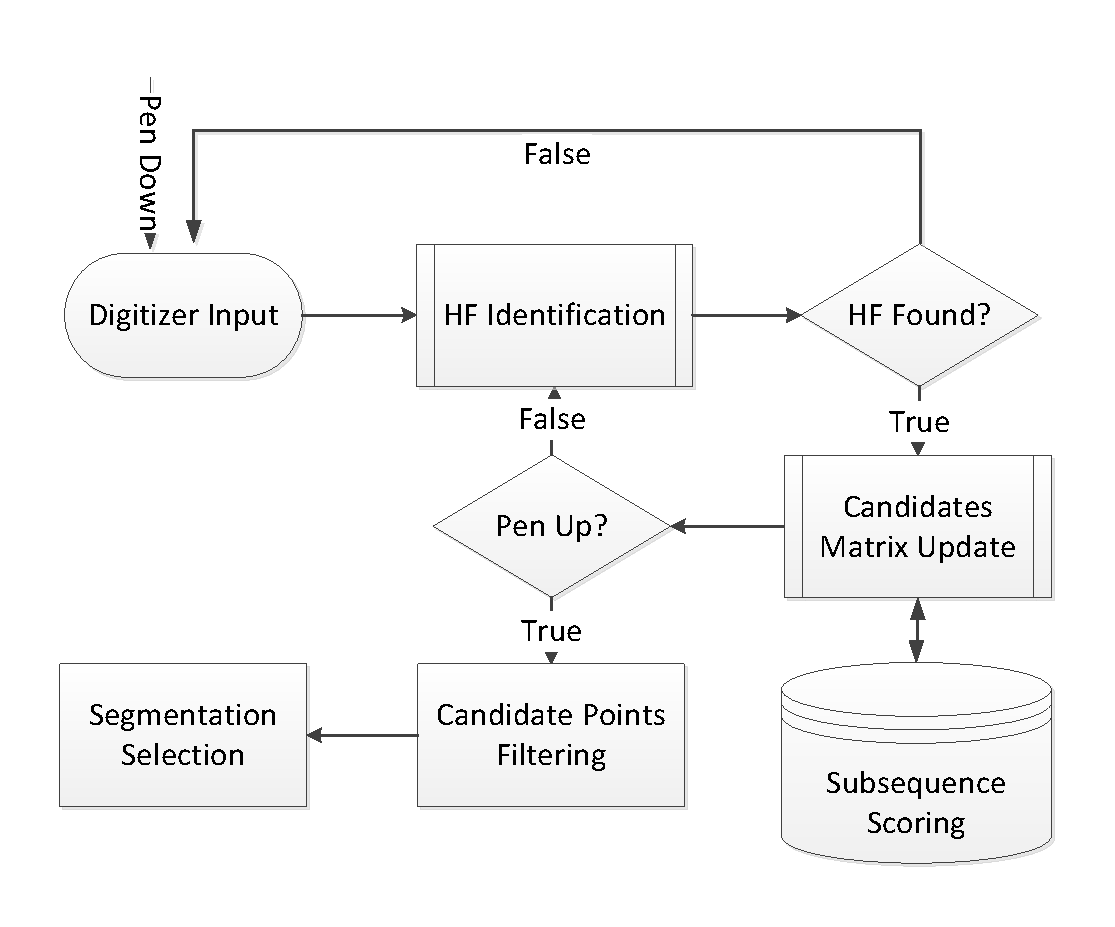
\includegraphics[width=0.8\textwidth]{./figures/system_flow}
\caption{High level visualization of segmentation flow.}
\label{fig:system_flow}
\end{figure}

%%%%%%%%%%%%%%%%%%%%%%%%%%%%%%%%%%%%%%%%%%%%%%%%%%%%%%%
\newpage{}
%%%%%%%%%%%%%%%%%%%%%%%%%%%%%%%%%%%%%%%%%%%%%%%%%%%%%%%

\section{First Stage: POIs Nomination and Sub-strokes Scoring}

\subsection{Horizontal fragment identification} 
In this stage, the system attempts to identify HFs that join pairs of connected letters. 
These handlers are horizontal, directed right to left and located near the baseline (see Figure  \ref{fig:horizontal_fragments}). 
Using a smoothed version of the trajectory helps the process to ignore undesired small horizontal regions that are frequently caused by the digitizer's imperfection.  
A point $p_{i}$ is defined as a "horizontal point" if the slope of the line $\overline{p_{i-1}p_{i}}$ is less than a pre-set value $\delta$, which was empirically tuned to $0.6$. 
The same exact value for this parameter was found independently in \cite{daifallah2009recognition}.

\begin{figure}
\centering
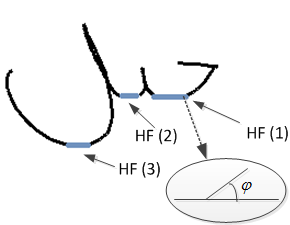
\includegraphics[width=0.3\columnwidth]{./figures/horizontal_fragments}
\caption{Horizontal Fragments (HFs) of the word \RL{jbl} /JABAL/.}
\label{fig:horizontal_fragments}
\end{figure}

HFs are continuously identified using the following process.
The first detected horizontal point is set as an "HF starting point". 
All the subsequent horizontal points are ignored until a non-horizontal point is detected, indicating the end of an HF sequence. 
This point is identified as an "HF ending point" and the medial point of an HF is marked as POI. 
POIs are potential SPs, thus, this process yields an over-segmentation of the stroke. 
While false positive SPs can be easily removed in a latter stage, missed SPs cannot be easily recovered. 
Therefore, in order to minimize the miss-rate, this process is delicate and allows false HFs to be detected.

Once an HF is detected the sub-stroke that spans from the previous POI to the POI of the current HF is checked to make sure they do not reside on the same HF. 
Inn case they do, both HFs are rejoined to a single HF. 
This is done to avoid fractions of the same HF to identified as multiple HFs, 
The merging is done by evaluating the complexity measurement across the two consequent HFs, see Figure \ref{fig:candidate_in_no_horizontal}.

\begin{definition}
\textbf{Complexity measure} is a value that indicates the curvature degree of a given 2-D trajectory $T=\{p_i\}_{i=1}^{n}$. 
Preprocessing steps, which include simplification and re-sampling, are required to ensure invariance under scaling and data imperfections. 
The complexity measure is calculated by summing the parameters $\alpha_{k}$ computed for each inner point $p_k$ in $T$ for $2 \leq k \leq n-1$, i.e., 
\begin{equation}
CM(T)=\sum_{k=2}^{n-1}{\alpha_k}.
\end{equation}
where the parameter $\alpha_{k}$ is defined as $\alpha_{k}=\frac{\pi-\phi_{k}}{\frac{\pi}{6}}$ and $\phi_k=\angle(\overline{p_{k-1}p_{k}},\overline{p_{k}p_{k+1}})$.
\end{definition}

\begin{figure}
\centering
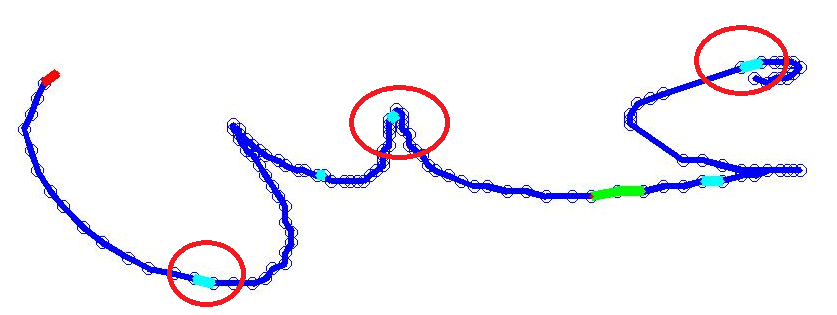
\includegraphics[width=0.3\textwidth]{./figures/candidate_in_no_horizontal}
\caption{The main body of Arabic word \RL{`yn} /AIN/. POIs are colored in cyan. The green areas indicate merge between two subsequent HFs. Three types of false POIs can be seen: 1. A POI at the beginning of a stroke. 2. A POI that is caused by a bad HF. 3. A POI that resides in a letter's valley. }
\label{fig:candidate_in_no_horizontal}
\end{figure}

\subsection{Sub-strokes scoring}
Let $S=\{p_{i}\}_{i=1}^{n}$ be a sequence representing a handwritten stroke in which $L$ POIs were detected. 
Let $KP=\{KP_{i}\}_{i=0}^{L+1}$ (Key points) be the ordered set of the POIs, in addition to the first and the last points of the stroke positioned as the first and the last items in the set.
Formally, we define: 
\begin{equation}
KP_{i} =\begin{cases}    1		, & \mbox{if } i=0 \\
					  POI_{i}	, & \mbox{if } 1\leq i \leq L \\
					       n    , & \mbox{if } i=L+1 
			\end{cases}				
\end{equation}
A sub-stroke $S_{i}^{j}$ is a sub-sequence of the stroke $S$ that starts at $KP_{i}$ and ends at $KP_{j}$, formally:
\begin{equation}
S_{i}^{j}=\{p_{k}\}_{k=KP_{i}}^{KP_{j}}; i<j
\end{equation}

We generate an upper triangular \emph{scoring matrix} $D\in\mathbb{R}^{(L+1)\times (L+1)}$ where each cell $D_{i,j}$ represents the sub-stroke $S_i^j$. 
It contains the classification information and scoring, for the sub-strokes $S_i^j$, returned by the characters classification system described in Chapter \ref{chap:characters_classification}. 
The matrix $D$ is generated dynamically; adding a row and a column for each new detected POI. 
Imposing a locality constraint which narrows the band of the $D$ matrix above the main diagonal improved the efficiency of the process and the segmentation accuracy. 
Given a band width $B$ we fix $D_{i,j}=\infty$ if  $j \leq i$ or $j-i>B$.
We argue that sub-strokes representing a letter will achieve, in most cases, better scoring, i.e., lower $D_{i,j}$ value than other sub-strokes.

\begin{figure}
\centering
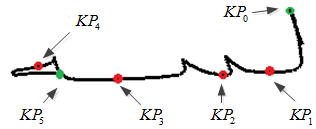
\includegraphics[width=0.4\textwidth]{./figures/candidate_points}
\caption{KPs of the word \RL{lbyh} /Lbyh/. POIs are coloured in red. The first and last KPs are coloured in green. }
\label{fig:candidate_points}
\end{figure}

Using the relative location of the sub-stroke in the stroke we restrict the classification process to search for similar samples feasible position databases.
As can be seen in Table \ref{table:subsequences_types}, we differentiate between four types of sub-sequences.
For each type, we indicate the set of databases that need to be examined, i.e., the possible letter positions the sub-stroke may represent. 
In Table \ref{table:subsequences_types}, $S$ denotes a stroke containing $L$ POIs where $m>0$ and $k<L+1$.

\begin{table}
\centering
\renewcommand{\arraystretch}{1.3}
\caption{A mapping between the subsequence types and the possible letter positions.}
\begin{tabular}{| c | c | c |}
\hline
  \textbf{Subsequence Symbol}     & \textbf{Subsequence Location}    & \textbf{Possible Letter Position}     \\
\hline
  $\alpha$ & $S_0^{k}$      & $Ini$ or $Mid$      \\
\hline
  $\beta$  & $S_{m}^{k}$    & $Mid$               \\
\hline
  $\chi$   & $S_{m}^{L+1}$ & $Mid$ or $Fin$       \\
\hline
  $\delta$ & $S_0^{L+1}$    & All                 \\
\hline
\end{tabular}
\label{table:subsequences_types}
\end{table}

The relation between the cells in the matrix $D$ and the sub-stroke type is given in matrix $D_p$  (Equation \ref{eq:positions_matrix}). 
The type of the sub-stroke can be determined while the stroke is being scribed.
The last column and row are added on the "pen up" event.

\begin{equation}
D_{p}=
\left( 
\begin{array}{ccccccc}
\infty 	& \alpha & \alpha & \alpha  & \cdots & \alpha & \delta      \\
\infty  & \infty  & \beta   & \beta   & \cdots  & \beta  & \chi     \\
\infty  & \infty  & \infty   & \beta   & \cdots  & \beta  & \chi    \\
\vdots & \vdots & \vdots  & \vdots & \ddots  & \vdots & \vdots      \\
\infty  & \infty  & \infty   & \infty   & \cdots  & \beta  & \chi   \\
\infty  & \infty  & \infty   & \infty   & \cdots  & \infty  & \chi  \\
\infty  & \infty  & \infty   & \infty   & \cdots  & \infty  & \infty \end{array} \right)
\label{eq:positions_matrix}
\end{equation}\\

For a given input (sequence and position), the recognition system returns the $K$ nearest neighbors with different labeling, where the labeling is defined as the tuple (letter, position). In our implementation, we set $K=3$.

\begin{figure}
\centering
\begin{tabular}{| c |c | c | c| c | c | c |}
\hline
     & $0$ & $1$ & $2$ & $3$ & $4$ & $5$\\
\hline
$0$
   & N/A
   & \subfloat{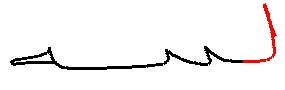
\includegraphics[width=1.8cm]{./figures/substrokes/L}}
   & \subfloat{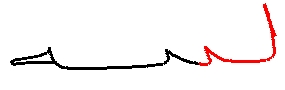
\includegraphics[width=1.8cm]{./figures/substrokes/LB1}}
   & \subfloat{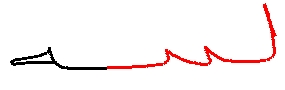
\includegraphics[width=1.8cm]{./figures/substrokes/LB1B2}}
   & N/A & N/A \\
\hline
$1$
   & N/A & N/A
   & \subfloat{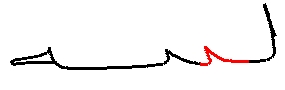
\includegraphics[width=1.8cm]{./figures/substrokes/B1}}
   & \subfloat{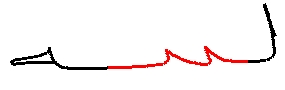
\includegraphics[width=1.8cm]{./figures/substrokes/B1B2}}
   & \subfloat{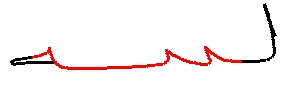
\includegraphics[width=1.8cm]{./figures/substrokes/B1B2H1}}
   & N/A \\
\hline
$2$
   & N/A  & N/A & N/A
   & \subfloat{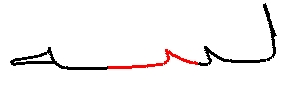
\includegraphics[width=1.8cm]{./figures/substrokes/B2}}
   & \subfloat{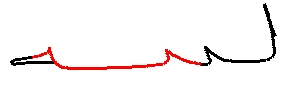
\includegraphics[width=1.8cm]{./figures/substrokes/B2H1}}
   & \subfloat{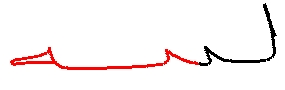
\includegraphics[width=1.8cm]{./figures/substrokes/B2H}} \\
\hline
$3$
   & N/A & N/A & N/A & N/A
   & \subfloat{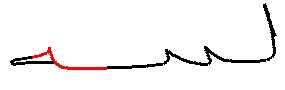
\includegraphics[width=1.8cm]{./figures/substrokes/H1}}
   & \subfloat{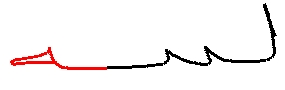
\includegraphics[width=1.8cm]{./figures/substrokes/H}} \\
\hline
$4$
   & N/A & N/A & N/A & N/A & N/A
   & \subfloat{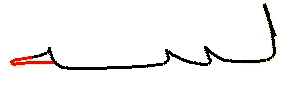
\includegraphics[width=1.8cm]{./figures/substrokes/H2}}\\
\hline
$5$
   & N/A & N/A & N/A & N/A & N/A & N/A \\
\hline
\end{tabular}
\caption{A tabular representation of the $D$ matrix that corresponds the KPs showed in Figure \ref{fig:candidate_points}. Each cell visually demonstrates the matching sub-stroke colored in red.}
\label{table:substrokes_demo} 
\end{figure}

%%%%%%%%%%%%%%%%%%%%%%%%%%%%%%%%%%%%%%%%%%%%%%%%%%%%%%%
\newpage{}
%%%%%%%%%%%%%%%%%%%%%%%%%%%%%%%%%%%%%%%%%%%%%%%%%%%%%%%

\section{Second Stage: POI Filtering and Scoring Correction}
In this stage we re-score subsequences and eliminate redundant POIs based on the following rules:

\begin{compactitem}
	\item SPs should lie close to the baseline. 
	\item SPs do not reside in loops.
	\item The sub-stroke length should be proportional to the length of the containing stroke.
\end{compactitem}

The system determines the baseline by calculating the vertical projection histogram of the re-sampled and normalized version of the stroke. 
The height of the stroke (y-axis) is partitioned into ten equi-length intervals. 
A POI is filtered out if it does not satisfy the following condition:
\begin{equation}
|POI_y-I_{max}| \leq 2 max{({|I|},0.15)} 
\end{equation}
where $POI_y$ represents the $y$-coordinate of the POI; $|I|$ is the length of an interval; and $I_{max}$ denotes the center of the most inhabited interval. 
In order to reliably determine the baseline, the baseline detection algorithm is activated only after the fourth POI is detected.
This process has proven to be very effective in eliminating challenging false POIs that reside in valleys of frequently used final Arabic letters, such as \RL{-q}, \RL{-s} and \RL{-n}. 
An example of such a POI can be seen in the letter \RL{-n} in Figure \ref{fig:candidate_in_no_horizontal}. 
Determining the baseline using the vertical projection histogram is a commonly used technique \cite{burrow2004arabic, bagdanov1997projection}.


The baseline is needed only to verify that the POIs are in a reasonable distance from it, therefore, imprecise valuation of the position or the direction of the baseline is tolerable.

\begin{figure}[b]
\centering

\includegraphics[width=0.8\textwidth]{./figures/baseline}
\caption{The position of the baseline corresponds to the largest peak of the vertical projection histogram \cite{burrow2004arabic}.}
\label{fig:candidate_in_no_horizontal}
\end{figure}

In order to identify SPs that resides inside a loop we have employed a Matlab package that includes an implementation for poly-line intersection algorithm \cite{legland2014geom2d}.

The third rule is used to penalize unreasonably low scoring given to small sub-strokes, which are unlikely to represent a letter. 
This is done by calculating the ratio of the sub-stroke length proportional to the entire stroke length.
For instance, it is common to add a small, hook-like, extension to the suffix of the letter \RL{d}. 
This extension may look very similar to the letter \RL{-a} during the stroke scribing; and thus under-scored, i.e. is given a very good similarity measure by the recognition system, and eventually result in over-segmenting the letter \RL{d}. 

In some cases, POIs are incorrectly nominated on non-horizontal areas. This is caused due to noises in the data and the fact that the nomination is done while the word is being scribed. Our filtering algorithm should be corrected, in a future work, to handle this case.

%%%%%%%%%%%%%%%%%%%%%%%%%%%%%%%%%%%%%%%%%%%%%%%%%%%%%%%
\newpage{}
%%%%%%%%%%%%%%%%%%%%%%%%%%%%%%%%%%%%%%%%%%%%%%%%%%%%%%%

\section{Third Stage: Segmentation Selection}
The goal of this phase is to select the set of SPs among the POIs. 
This set will be referred to as the \emph{final segmentation points} (FSP). 
It is performed by finding the \emph{segmentation path} in $D$ with the best scoring possible. 
A segmentation path $\pi$ is an ordered subset of the KPs and must contain $KP_{0}$ and $KP_{L+1}$ as the first and the last points in the path.
$\Pi$ denotes the scoring of the segmentation path $\pi$. 
It is defined as the summation of the sub-sequences scoring in the segmentation path divided by the path length; this is done in order to prevent giving superiority to under-segmentations.

One can model the scoring matrix $D$ as a directed, edge-weighted graph $G=(V,E)$, for which a path from vertex $KP_0$ to vertex $KP_{L+1}$ defines a possible segmentation. 
It can be experimentally validated that finding the shortest path in $G$ (from $KP_0$ to $KP_{L+1}$) does not necessarily obtain the optimal segmentation, and in some cases, produces under-segmentation of the stroke. 
It is because the shortest path is a global property, which may prefer a highly weighted shortcut path over a path that consists of several low weighted fragments; in cases where the accumulative weight of the fragmented path is larger than the shortcut path.
However, greedily selecting the outgoing edge with the minimal weight will mostly return a better segmentation.

Several \emph{segmentation selection algorithms} (SSAs) for finding the best segmentation path are proposed in this work.
Here we describe two algorithms that were given the names \emph{Forwards Segmentation Selection} (FSS) and \emph{Backwards Segmentation Selection} (BSS) which operate quite similarly. 
A pseudo-code of FSS algorithm can be seen in Algorithm \ref{alg:fss}. 
FSS starts with the first point, $KP_0$, advancing toward the end of the stroke. 
In Each step, it tries to find the next best KP by selecting the adjacent subsequence $S_i^j$ with the best scoring (as can be seen in line 5). 
BSS operates similarly but starts from the last point and advances toward the beginning of the stroke. 
The main drawback of these two algorithms is that FSS tends to under-segment the suffix of the stroke and BSS tends to under-segment the stroke's prefix.

\begin{algorithm}
$\pi = \{0\} $\;
$i=0$\;
$sum=0$\;
\While{$i<L+1$}
{
	$j = \mathop {\arg \min }\limits_k \left( {D\left( {i,k} \right)} \right)$\;
	$\pi = \pi \cup \left\{ j \right\}$\;
	$sum = sum + D\left( {i,j} \right)$\;
	$i=j$\;
}
\caption{Forwards Segmentation Selection (FSS) algorithm.}
\label{alg:fss}
\end{algorithm}

In an attempt to overcome the aforementioned drawbacks, a third SSA is proposed, and given the name \emph{Backwards-Forwards Segmentation Selection} (BFSS). 
As can be seen in Algorithm \ref{alg:bfss}, it combines both FSS and BSS. 
BFSS operates from the sides of the stroke toward the center. In every iteration, it selects two candidate points to include to the segmentation path.

\begin{algorithm}
$\pi = \{0,L+1\}$\;
$kp_{a}=0$\;
$kp_{b}=L+1$\;
\While{$kp_{a}<kp_{b}$}
{
	$kp_{a,next} = \mathop {\arg \min}\limits_k (D(kp_a,k))$\;
	$\pi = \pi \cup \{kp_{a,next}\}$\;
	$kp_{a}=kp_{a,next}$\;
	
	$kp_{b,next} = \mathop {\arg \min}\limits_k (D(k,kp_{b,next}))$\;
	$\pi = \pi \cup \{kp_{b,next}\}$\;	
	$kp_{b}=kp_{b,next}$\;
}
\caption{Backwards-Forwards Segmentation Selection (BFSS) algorithm.}
\label{alg:bfss}
\end{algorithm}
  
The last algorithm was given the name \emph{Greedy Segmentation Selection} (GSS) and is described in Algorithm \ref{alg:gss}.
GSS operates differently. In every iteration, the cell with the lowest (best) scoring is selected. 
Once a cell $D_{i,j}$ is selected, since it represents the sub-stroke $S_{i}^{j}$, both $KP_{i}$ and $KP_{j}$ are added to the FSP, and every cell corresponding to a subpart of the sub-stroke $S_{i}^{j}$ is removed by setting its corresponding scoring value in the matrix $D$ to $\infty$; in order to avoid those sub-strokes to be selected in a later iteration. In Algorithm \ref{alg:gss}, the notation $[\infty]^{(L+1)\times (L+1)}$ indicates a matrix that all it's cells are set to $\infty$.
 
\begin{algorithm}
$\pi = \{0,L+1\}$\;
\While{$D \neq [\infty]^{(L+1)\times (L+1)}$}
{
	${s,e} = \mathop {\arg \min}(D)$\;
	$\pi = \pi \cup \{s,e\}$\;
	$sum = sum + D(s,e)$\;
	$UpdateMatrix(D,s,e)$\;
}

\caption{Greedy Segmentation Selection (GSS) algorithm.}
\label{alg:gss}
\end{algorithm}

Performance evaluation of the mentioned SSA is provided in \ref{subsec:ssa_performance}.


%%%%%%%%%%%%%%%%%%%%%%%%%%%%%%%%%%%%%%%%%%%%%%%%%%%%%%%
\newpage{}
%%%%%%%%%%%%%%%%%%%%%%%%%%%%%%%%%%%%%%%%%%%%%%%%%%%%%%%

\section{Experimental Results}
\label{sec:segmentation_results}
Comparing the performance of the real-time segmentation approach described in this work to results obtained by related researches is difficult due to the different experimental settings, databases and methodology; not to mention the different measures used to present the results. 
The usage of the ADAB database, instead of a self-collected database, standardize and reinforces our results. 
In Table \ref{table:general_stats}, we provide basic statistics of our sample set. 
Table \ref{table:segmentation_results} summarizes the system's performance.

\begin{table}[b]
\renewcommand{\arraystretch}{1.2}
\centering
\caption{Segmentation sample set general statistics.}
\begin{tabular}{ | c | c | }
  \hline
  Number of test samples (city name) & 319 \\
  \hline
  Number of WPs & 1148 \\
  \hline
  Number of Strokes & 1237 \\
  \hline
\end{tabular}
\label{table:general_stats} 
\end{table}

\begin{table}[b]
\renewcommand{\arraystretch}{1.2}
\centering
\caption{Segmentation results.}
\begin{tabular}{ | c | c | }
  \hline
  Strokes segmentation rate &  83\% \\ 
  \hline
  Strokes recognition rate &  78\% \\ 
 \hline
  Total number of true SPs & 1081 \\
  \hline
  Valid SPs (True Positive) & 85.3\% \\
    \hline
  Missing SPs (False Negative) & 14.7\% \\
  \hline
  Invalid SPs (False Positive) & 119 (11\%) \\
  \hline                                    
  SPs Precision & 88.6\% \\ 
 \hline
  SPs Recall &  85.3\% \\ 
 \hline
\end{tabular}
\label{table:segmentation_results} 
\end{table}

\subsection{Validation}
\label{subsec:validation}
Related researches usually use a human expert to validate the accuracy of the SPs. However, in this work, we applied an automatic validation process using the ground truth information provided by the database. We discriminate between three types of final SPs. A final SP is classified as true positive if the complexity measure between the identified point and a true SP is less than a preset threshold; otherwise, it is classified as false positive. A false negative (miss), is the case when the system failed to identify a true SP. The different types of SPs can be seen in Figure \ref{fig:sp_types}.
The validation process was tested on several sets and found to be highly reliable.

\begin{figure}[b]
\centering
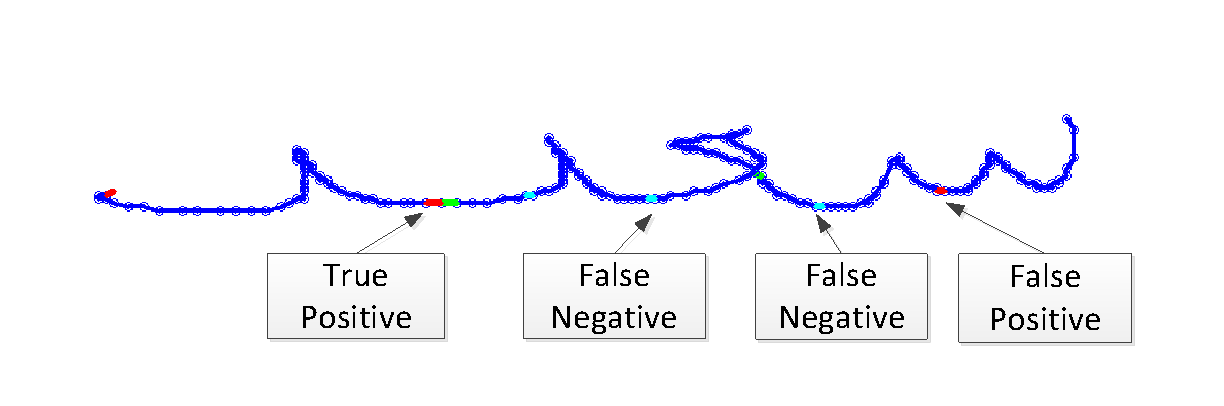
\includegraphics[width=0.6\textwidth]{./figures/sp_types}
\caption{SPs types.}
\label{fig:sp_types}
\end{figure}

\subsection{Analysis}
In this section we discuss common cases of incorrect segmentation.\\
\subsubsection{Over-segmentation}
\begin{itemize}
\item Several Arabic letters contain a horizontal region in their initial form which does not accommodate a SP, see Figure \ref{fig:candidate_in_no_horizontal}. 
We overcame this problem by adding the following rule: a POI is nominated only if the sub-stroke that spans from the beginning of the stroke to the POI has a high complexity measure.
\item Over-segmentation can also be caused by typing a letter in unusual form where it is spanned over several strokes. 
It happens mostly in the letter \RL{-m-}, \RL{-m} and in rare cases in the letter \RL{-.h-}. This issue will be addressed in a future work.
\end{itemize}

\begin{figure}
\centering
        \subfloat[]{
            \label{fig:letters_same_body_1}
            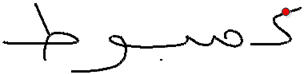
\includegraphics[width=0.3\textwidth]{./figures/oversegmentation_begin_1}
        }
        \subfloat[]{
           \label{fig:letters_same_body_2}
           
\includegraphics[width=0.15\textwidth]{./figures/oversegmentation_begin_2}
        }        
    \caption{Samples of redundant Candidate point at the beginning of the stroke.}
   \label{fig:oversegmentation_begin}
\end{figure}

Without the additional strokes, there is no way to differentiate between the main body of the letter \RL{-s-} /s/ and the main body of two consecutive \RL{-b-} /b/ (or other identical main body letters as seen in figure \ref{fig:same_body_letters}). 


\begin{figure}
\centering
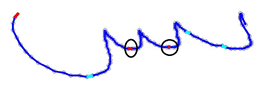
\includegraphics[width=5cm]{./figures/oversegmentation_s}
\caption{Over-segmentation in the letter \RL{-s-}. appearance to a combination of two consecutive \RL{-b-} letters and only can be identified from the context and using the additional strokes.}
\label{fig:oversegmentation_s}
\end{figure}

\subsubsection{Under-segmentation}
\begin{itemize}
\item Letter pairs that are not separated by HFs cause the system to miss POIs. This was partially solved by extending the notion of a letter to include such pairs. For example the pair \RL{lm} and \RL{l.h}.
\item In some cases, HFs were identified correctly but the corresponding POI were not selected in the third stage. This may result from nomination of a candidate point on correct horizontal segment but in a late fraction of the segmentation fragment which result in a low scoring and thus not being selected by the SSA. This issue usually occurs in the letter \RL{w} in its final position (Figure \ref{fig:undersegmentation_w}).
\end{itemize}

\begin{figure}
\centering
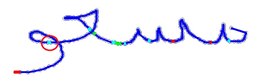
\includegraphics[width=5cm]{./figures/undersegmentation_w}
\caption{An example of a late candidate point in the letter \RL{w}.}
\label{fig:undersegmentation_w}
\end{figure}

We have noticed that the absolute majority of the false negative (missed) SPs were actually identified as POIs in the first stage, but were not selected by the SSA.
In addition, differentiating between the main body of the letter \RL{-s-} and the main body of two consecutive \RL{-b-} letters is possible only when considering the additional strokes, thus both cases were considered to be correct.

\subsection{Segmentation Selection Algorithms Performance}
\label{subsec:ssa_performance}
It is apparent from the data in Table \ref{table:ss_algorithms_results}, that the SSA has a crucial effect on the system's performance. 
We tested several combinations of two SSAs in which the FSP is found by executing both SSAs independently and selecting the segmentation path with the smallest scoring. In Table \ref{table:ss_algorithms_results}, a combination of two algorithms is denoted by $\oplus$.

\begin{table}
\centering
\caption{Comparing the different SSAs performance.}
\begin{tabular}{ | c | c | c | c | c |}
\hline
\textbf{SSA} & \textbf{WP segmentation} & \textbf{WP recognition} & \textbf{SP precision} & \textbf{SP recall}\\
             & \textbf{rate}            & \textbf{rate}           &                       &\\  
\hline                 
  FSS & 76\% & 70\% & 85\% & 78\% \\ 
  \hline
  BSS & 79\% &  73\% & 84\%& 81\% \\
  \hline
  BFSS & 78\% & 72\% & 84\% & 80\%\\ 
  \hline
  GSS & 80\% & 74\% & 81\% & \bf{94}\% \\  
  \hline
  FSS$\oplus$BSS & \bf{82}\% & \bf{76}\% & \bf{89}\% & 82\%\\  
  \hline
  GSS$\oplus$BFSS & 81\% & 75\% & 83\% & 90\% \\
  \hline
\end{tabular}
\label{table:ss_algorithms_results} 
\end{table}

\subsection{Sample set size and distribution}
The letters is our training set are extracted from a database with a limited words diversity, thus, the distribution of the samples between the different classes is imbalanced. 
On one hand, it can be regarded as an advantage; since, the training set distribution reflects the a-priory probability of a letter appearance in the test set. 
On the other hand, a highly imbalanced training set is known to negatively affect many classification algorithms.
In the following experiment, we measure the effect of a large and imbalanced training set on the WP segmentation and recognition rates. 
It is done by gradually increasing the maximal allowed number of samples per class (letter and position).
 
The graph in Figure \ref{fig:num_letter_impact} shows convergence of the system's performance when the maximal number of samples is larger than 200 per class. 
Nevertheless, a miniature degradation is apparent, which is caused, probably, due to the increasing imbalance in the distribution of the training set.
In addition, it is evident that the recognition rate is more sensitive to small training set than the segmentation rate.

\begin{figure}
\centering
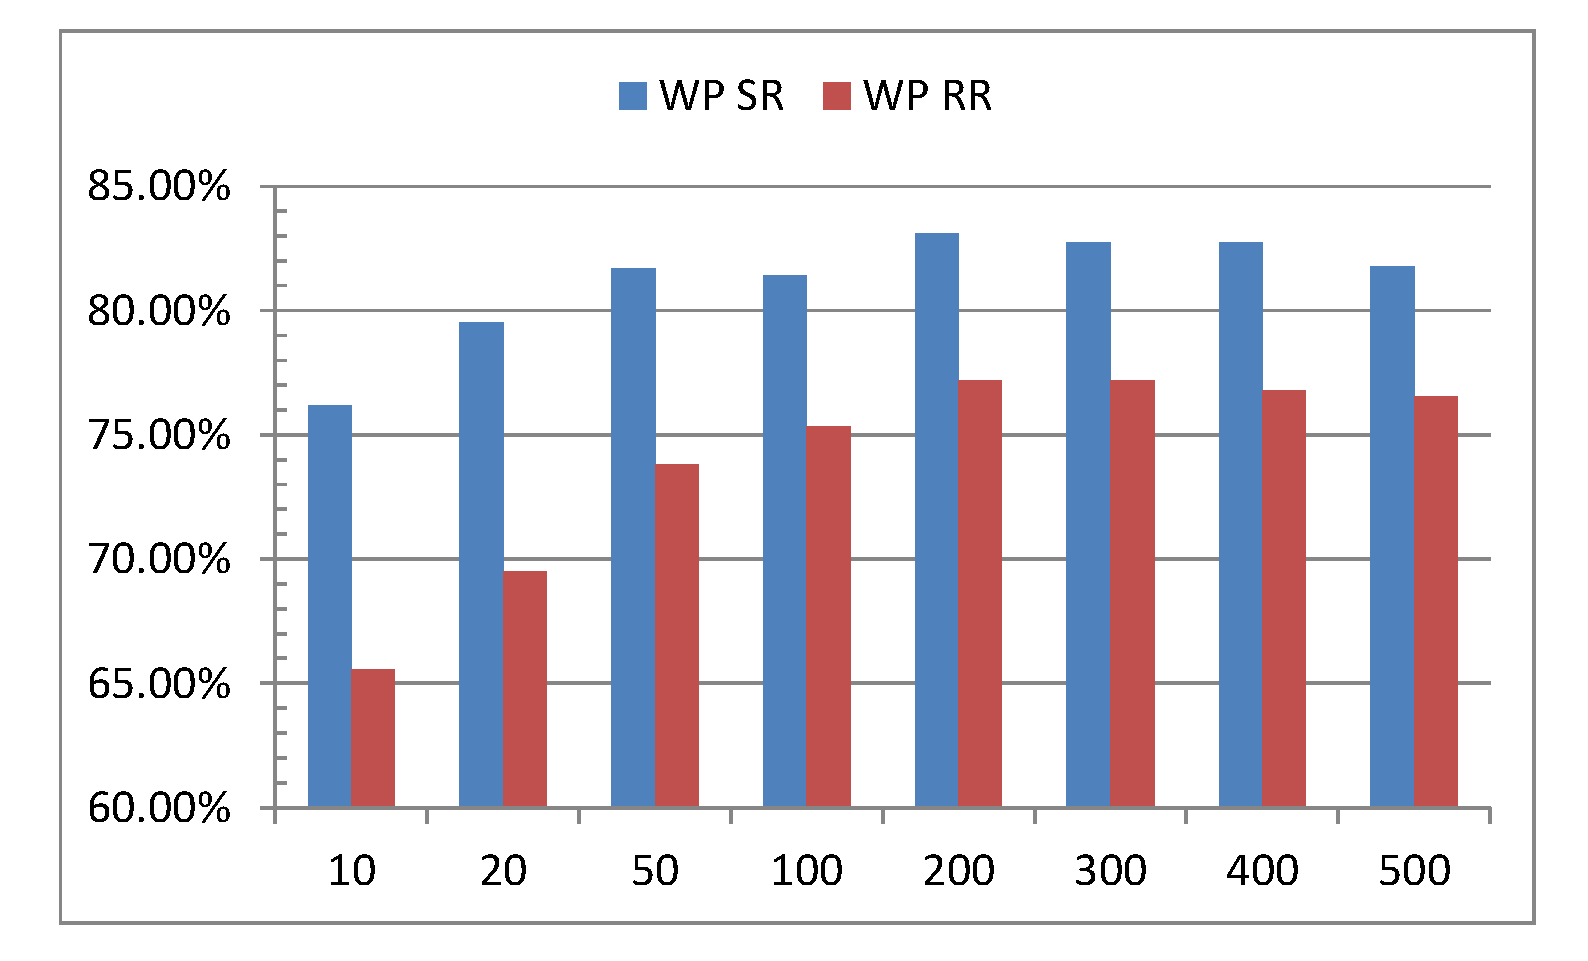
\includegraphics[width=0.7\textwidth]{./figures/num_letter_impact}
\caption{The impact of increasing the maximal number of samples per class on the segmentation and recognition rates.}
\label{fig:num_letter_impact}
\end{figure}

%%%%%%%%%%%%%%%%%%%%%%%%%%%%%%%%%%%%%%%%%%%%%%%%%%%%%%%
\newpage{}
%%%%%%%%%%%%%%%%%%%%%%%%%%%%%%%%%%%%%%%%%%%%%%%%%%%%%%%

\section{Holistic WPs Recognition Using Characters Classification Information}
\label{sec:wps_recognition}
As mentioned earlier, the segmentation and classification information obtained by a real-time segmentation system, can be used to significantly reduce the potential dictionary size and accelerate a later holistic recognition process as follows:
\begin{compactitem}
\item In an open-vocabulary environment, the classification information can be employed to dynamically build a class of different shapes for all possible WPs.
\item In a closed-vocabulary environment, a holistic recognition approach can be limited to consider valid combination that appear in the vocabulary. 
\end{compactitem}

In this section we evaluate the recognition accuracy that can be obtained in the an open-vocabulary environment.
Following the real-time segmentation process, the $10$ top scored candidates of each character are recorded. 
These shapes are used to generate a complete list of all possible shape concatenation of the retrieved candidates. 
The obtained candidates represent different shapes of the same letter producing multiple shapes of the same WP. 
The cardinality of the generated list is $10^p$ where $p$ is the predicted number of characters in the WP using the segmentation process. 
The large size of the generated list, which may exceed $10,000$ shapes, requires a similar process of embedding and dimensionality reduction, as described above, to generate a short list of candidates. 
The short list of candidates in the next step is matched against the queried WP using the original expensive and more accurate matching process. 
Using the proposed approach, the $10$ top WPs results yield a $98.1\%$ recognition rate. 
The recognition rate of the first top candidate dropped down to $90.8\%$. 
Using a voting process within the top five results gave a $94.7\%$ recognition rate. 

Analysing the failures of the misclassified samples shows that most recognition errors occur as a result of misclassifying a single character. 
In most cases the misclassified character is confused with a character having a very similar shape, which can be corrected using information retrieved by the associated additional stroke, such as the case of the letter \RL{-l} /l/ and the letter \RL{-n} /n/ in their handwritten form.


%\bibliographystyle{plainnat}
%\bibliography{references}
%
%\end{document}

%\documentclass[12pt,english]{report}
%\usepackage{mathptmx}
%\renewcommand{\familydefault}{\rmdefault}
%\usepackage[T1]{fontenc}
%\usepackage[latin9]{inputenc}
%\usepackage[a4paper]{geometry}
%\setcounter{secnumdepth}{2} % Changed from 3 to 2. 0-chapter 1-section 2-subsection 
%\setcounter{tocdepth}{2} % Changed from 3 to 2. 0-chapter 1-section 2-subsection 
%\setlength{\parskip}{\medskipamount}
%\setlength{\parindent}{0pt}
%\usepackage{verbatim}
%\usepackage{pdfpages}
%\usepackage{graphicx}
%\usepackage{subfig} %% This package has to be here
%\usepackage{setspace}
%\usepackage{arabtex}
%\usepackage[numbers]{natbib}
%\usepackage{nomencl}
%\usepackage{amsthm}
%\usepackage{amsmath}
%\usepackage{amsfonts}
%\usepackage{paralist}
%\usepackage{etoolbox}
%\newtoggle{edit-mode}
%\toggletrue{edit-mode}  
%%%\toggletrue{edit-mode}
%\iftoggle{edit-mode}{
%\geometry{verbose,tmargin=2cm,bmargin=2cm,lmargin=2cm,rmargin=6cm,headheight=1cm,headsep=1cm,footskip=1cm, marginparwidth=5cm}
%}{
%\geometry{verbose,tmargin=2cm,bmargin=2cm,lmargin=2cm,rmargin=2cm,headheight=1cm,headsep=1cm,footskip=1cm}
%}
%
%
%\begin{document}

\chapter{Summary and Future Work}
\label{chap:summary}

\section{Summary}
\label{sec:summary}

The cursiveness of the Arabic script, prima facie, requires delaying the launch of the recognition process until the completion of the word scribing. 
However, in this study, we question the necessity of the requirement by demonstrating the feasibility of determining the position of the segmentation points while the stroke is being written; and by doing so, accelerating the recognition process.

The proposed recognition-based segmentation method is performed in the stroke level enabling analysis task related to segmentation and recognition of the stroke to be performed in real-time. 
The first stage, which requires the most calculation effort, is performed whilst the stroke is being written and involves over-segmentation of the stroke.
Morphological features are employed to nominate potential SPs.
The sub-strokes induced by the SPs are classified using a fast character classifier, and the classification information is saved in a scoring matrix.
The second stage contains filtering of the topologically invalid SPs. 
The last stage involves several segmentation points selections algorithm which determines the best subset of segmentation points.

The real-time nature of the segmentation system requires implementing a fast Arabic handwritten characters classifier.
The proposed classifier include preprocessing stage followed by a features extraction process, employing the SC and the MAD descriptors, to extract features from each significant point on the stroke.
Using an efficient EMD embedding into the wavelet coefficient domain, the feature vectors were translated into the $L_1$ space, facilitating fast approximation of the EMD metric.
A combination of PCA and LDA was employed to reduce the dimensionality of the sparse vectors generated by the embedding function.
Fast retrieval of the $k$ nearest neighbours was then possible using fast using $k$-d tree.
DTW was used to refine the similarity scoring of the candidates.
We proposed several activation configurations of the classification approach aiming at finding the desired balance between accuracy and response time.

The system has been designed and tested using the ADAB Database, a publicly available corpus of on-line Arabic handwriting.
We have built large database of handwritten Arabic letters and WPs based on the strokes information given in the database, overcoming absence of mapping between the strokes and letters in the ADAB database.
We have used the skills of a human expert to manually segmenting of the strokes trajectories and mark the WPs boundaries.

Extensive experiments and detailed analysis was given on both the classification and the segmentation systems.
Then, we showed that the characters classification information obtained by a real-time segmentation system can be used to significantly accelerate a later holistic WPs recognition process.


%%%%%%%%%%%%%%%%%%%%%%%%%%%%%%%%%%%%%%%%%%%%%%%%%%%%%%%
\newpage{}
%%%%%%%%%%%%%%%%%%%%%%%%%%%%%%%%%%%%%%%%%%%%%%%%%%%%%%%

\section{Future Directions}
\label{sec:future_directions}

In future work, we will expand the process by adding a later holistic word part recognizer that exploits the proposed segmentation and the scoring information to inspect a limited number of potential word parts.
Also, we are planning to allow the letter writing to be expand over multiple strokes.
In addition we will develop a word completion algorithm based on our real-time recognition technique.

In a future work, the additional strokes will be employed to discriminate between letters having the same main body (i'jam).
We believe that this will significantly improve the segmentation and classification results, as the additional strokes can help decrease the potential letter set.

We are planning to enhance the segmentation points nomination by employing morphological learning algorithm for determining if the given point is a potential segmentation point based on the surrounding environment of the candidate point. 

In addition are planning to standardize and publish the characters database extracted from the ADAB database and make available for other researches in the field.

%\end{document}

\bibliographystyle{plainnat}
\bibliography{references}

\appendix

%% LyX 2.0.5.1 created this file.  For more info, see http://www.lyx.org/.
%% Do not edit unless you really know what you are doing.
%\documentclass[12pt,english]{report}
%\usepackage{mathptmx}
%\renewcommand{\familydefault}{\rmdefault}
%\usepackage[T1]{fontenc}
%\usepackage[latin9]{inputenc}
%\usepackage[a4paper]{geometry}
%\setcounter{secnumdepth}{2} % Changed from 3 to 2. 0-chapter 1-section 2-subsection 
%\setcounter{tocdepth}{2} % Changed from 3 to 2. 0-chapter 1-section 2-subsection 
%\setlength{\parskip}{\medskipamount}
%\setlength{\parindent}{0pt}
%\usepackage{verbatim}
%\usepackage{pdfpages}
%\usepackage{graphicx}
%\usepackage{subfig} %% This package has to be here
%\usepackage{setspace}
%\usepackage{arabtex}
%\usepackage[numbers]{natbib}
%\usepackage{nomencl}
%\usepackage{amsthm}
%\usepackage{amsmath}
%\usepackage{amsfonts}
%\usepackage{paralist}
%\usepackage{etoolbox}
%\newtoggle{edit-mode}
%\toggletrue{edit-mode}  
%%%\toggletrue{edit-mode}
%\iftoggle{edit-mode}{
%\geometry{verbose,tmargin=2cm,bmargin=2cm,lmargin=2cm,rmargin=6cm,headheight=1cm,headsep=1cm,footskip=1cm, marginparwidth=5cm}
%}{
%\geometry{verbose,tmargin=2cm,bmargin=2cm,lmargin=2cm,rmargin=2cm,headheight=1cm,headsep=1cm,footskip=1cm}
%}
%
%\makenomenclature
%
%%% Theorem Styles
%\newtheorem{theorem}{Theorem}[section]
%%% Definition Styles
%\theoremstyle{definition}
%\newtheorem{definition}{Definition}[section]
%\newtheorem{example}{Example}[section]
%\theoremstyle{remark}
%\newtheorem{remark}{Remark}
%
%\usepackage[linesnumbered]{algorithm2e}
%
%\begin{document}

\chapter{Data Collection and Preparation}
\label{app:data_collection}

\section{The ADAB Database}
\label{sec:adab_database}

\iftoggle{edit-mode}{\hspace{0pt}\marginpar{The data importance}}{}
The data, its quality and quantity, are a fundamental part of any supervised machine learning technique.
It is used in the learning, validation and testing stages of the pattern recognition process, and has a critical effect on the system accuracy and performance.

\iftoggle{edit-mode}{\hspace{0pt}\marginpar{Data representation}}{}
On-line handwritten data is commonly a digitized representation of the pen movement. 
It may contain sequential information about position, velocity, acceleration, pressure, or even angle and orientation of the pen as a function of time. 
Nevertheless, the pen's position is the most commonly used property. 
Although the sampling of the pen position is done in a constant time intervals, the vast majority of HWR system do not use the temporal information but only consider the serial ordering of pen planar position. 

\iftoggle{edit-mode}{\hspace{0pt}\marginpar{Lack of databases}}{}
Many databases were developed for both on-line and off-line HWR of English script. 
Among these we can mention the following popular database: UNIPEN \cite{guyon1994unipen}, CEDAR \cite{hull1994database}, IRONOFF \cite{viard1999ireste} and NIST.
However, very few databases were developed for the Arabic script and are publicly available such as IFN/ENIT \cite{pechwitz2002ifn} and CEDAR \cite{srihari2005search}.
Thus, most researchers had developed their own private limited datasets \cite{saabni2009efficient}. 
Even fewer datasets were created for the on-line Arabic script. 
This shortage may be attributed to the fact that the major work done on Arabic handwriting recognition focused on recognizing off-line script \cite{plamondon2000online}.
Another reason may be the fact that most research in the on-line script recognition field is done for isolated characters such as letters, digits and symbols \cite{al2011online}.

\iftoggle{edit-mode}{\hspace{0pt}\marginpar{The ADAB database}}{}
In this work, we have used the only publicly available corpus of on-line Arabic handwriting, called the \emph{ADAB} (Arabic DAtaBase) database, which is de-facto a standard in this field \cite{el2009icdar}.
It was developed to advance the research and development of Arabic on-line handwritten text recognition systems and consists of more than 20k Arabic handwritten words scribed by more than 170 different writers.
The samples are words that were taken from the 937 Tunisian town/village names.
Each stroke, represented as a node in the XML, contains the sequence of $(x,y)$ coordinates of the pen position expanded from the pen-down to the corresponding pen-up event, as can be seen in Figure \ref{fig:adab_inkml}.
In addition to the strokes positional information of the stroke, the database contains several properties related to the equipment used to obtain the data and the writer's information, as well as the plot image of the word trajectory as shown in Figure \ref{fig:sample_parts}.

\begin{figure}
\centering
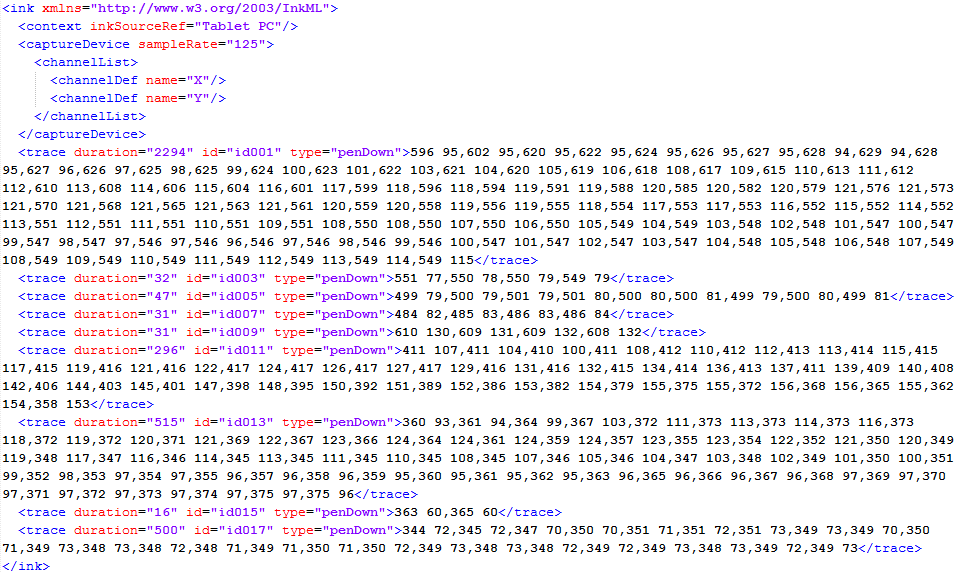
\includegraphics[width=1\textwidth]{./figures/adab_inkml}
\caption{Trajectory information of a city name sample.}
\label{fig:adab_inkml}
\end{figure}

\begin{figure}
\centering
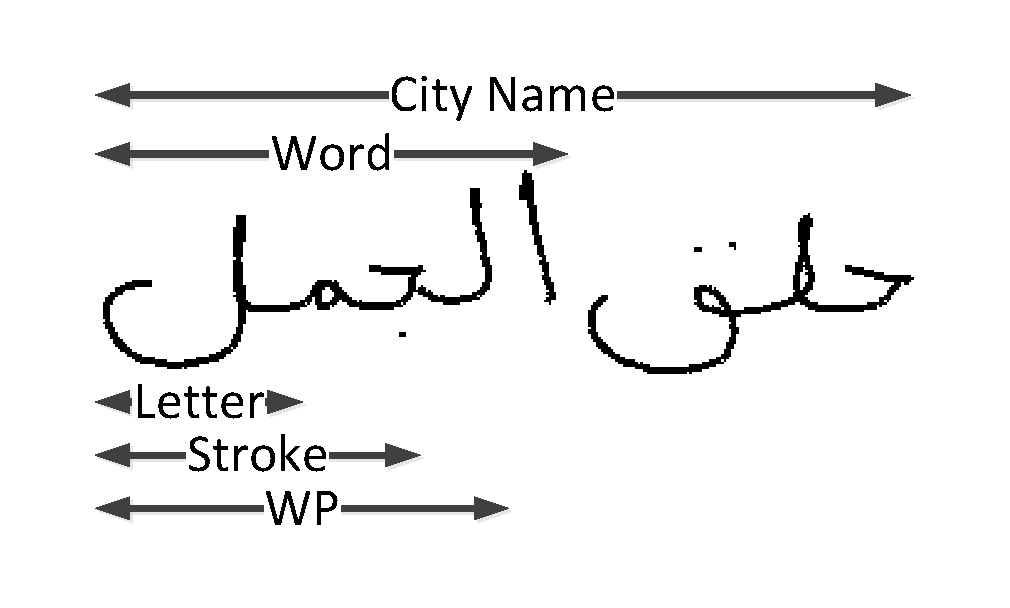
\includegraphics[width=0.4\textwidth]{./figures/sample_parts}
\caption{Visual demonstration of a test sample parts.}
\label{fig:sample_parts}
\end{figure}

%%%%%%%%%%%%%%%%%%%%%%%%%%%%%%%%%%%%%%%%%%%%%%%%%%%%%%%
\newpage{}
%%%%%%%%%%%%%%%%%%%%%%%%%%%%%%%%%%%%%%%%%%%%%%%%%%%%%%%

\section{Letter Samples Extraction}
\label{sec:letters_extraction}

\iftoggle{edit-mode}{\hspace{0pt}\marginpar{The missing information}}{}
The goal of this stage was to create a sufficiently large database of handwritten Arabic letters to be used by the letter classifier described in Chapter \ref{chap:classification}, and as a ground-truth for validating the segmentation method described in Chapter \ref{chap:segmentation}.
The absence of mapping between the strokes and letters in the ADAB database, required manual segmentation of the strokes trajectories.

\iftoggle{edit-mode}{\hspace{0pt}\marginpar{Letters extraction method}}{}
To facilitate the database construction, we have created a user friendly system that reads the samples from the ADAB database, displays the different strokes of a sample in different color, and enables a human expert to easily mark the segmentation points on the strokes.
Once the segmentation process is done, the match between the sub-strokes and the letters is performed in a semi-automatic manner, which required the expert intervention only in cases of ambiguity.  
The system was designed also to handle samples that included more than a single letter. 
In this case, the expert also had to relate the strokes to the different words.
The graphical user interface of the system is shown in Figure \ref{fig:manual_segmentation}. 

\begin{figure}[h]
\centering
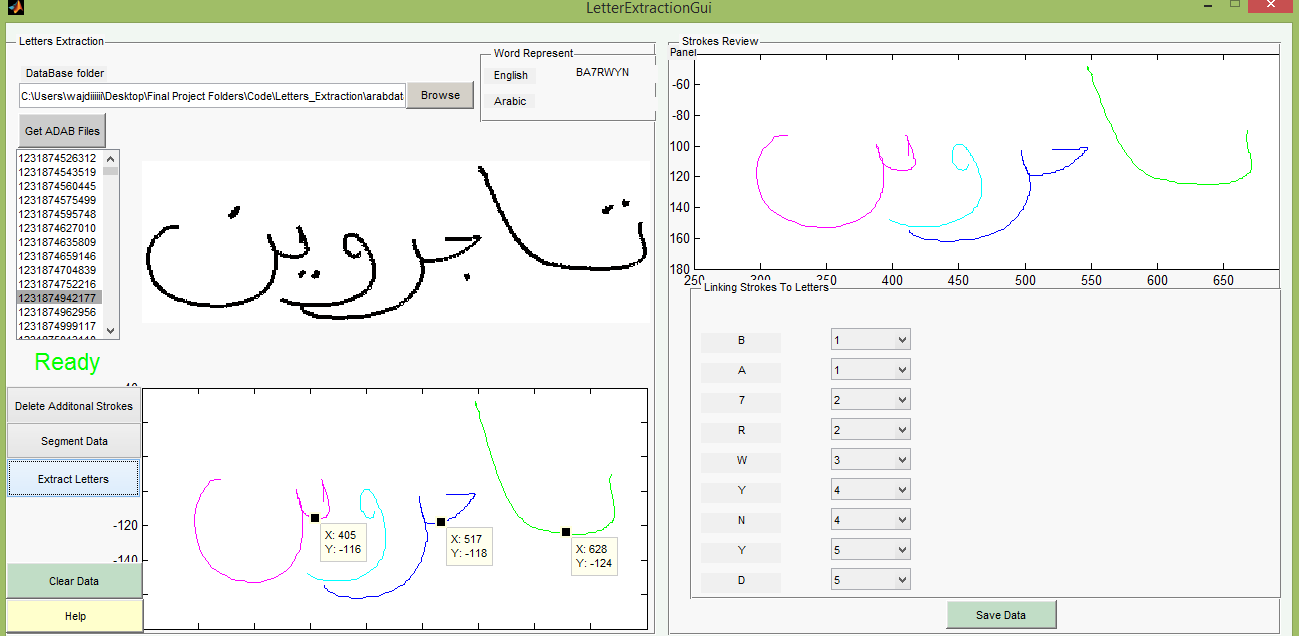
\includegraphics[width=1\textwidth]{./figures/manual_segmentation}
\caption{A view of manual segmentation system.}
\label{fig:manual_segmentation}
\end{figure}

\iftoggle{edit-mode}{\hspace{0pt}\marginpar{Additional strokes detection and removal}}{}
Since, neither the classification system nor the segmentation process consider the additional strokes, the system automatically filtered them out. 
The detection of delayed strokes was performed based on the stroke size and the area of its bounding box. 
However, in order to avoid unintentionally removing main bodies of small letters, we set a relatively high threshold.
Thus, the human expert had to filter out additional strokes manually that could not be identified by the system as such.

\iftoggle{edit-mode}{\hspace{0pt}\marginpar{The output structure}}{}
The output of the system was saved in a parsed XML file for each sample. 
As can be seen in Figure \ref{fig:adab_segmented_xml}, the hierarchy of the out XML represents the structure of the sample as defined in Figure \ref{fig:sample_parts}. 
In order to build up the letters database, an automatic procedure was implemented to extract the letters trajectories from the output XML. 
The letters database consists of directories that represent the different letters.
Each letter directory contains four folders, named Iso, Mid, Fin and Iso which contains the corresponding letter samples, recorded in a Matlab data files.
In the case of a dis-connective letter, the letter folder contains two directories representing the Iso and Mid forms of the corresponding letter.
For the sake of obtaining a sample-set sufficiently large to be used for both learning and validation, more than 7k samples were manually segmented which consisted of about 20k letters. 

\begin{figure}
\centering
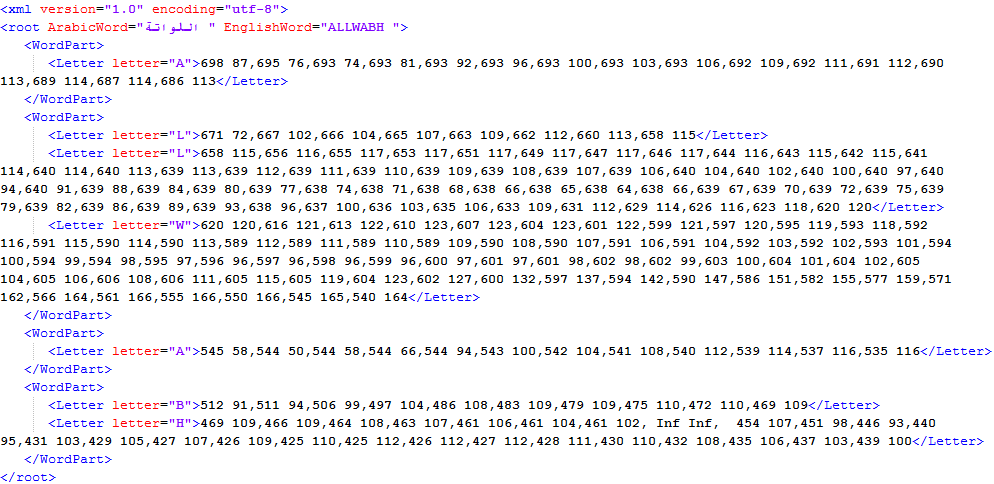
\includegraphics[width=1\textwidth]{./figures/adab_segmented_xml}
\caption{The output parsed  XML.}
\label{fig:adab_segmented_xml}
\end{figure}

%\bibliographystyle{plainnat}
%\bibliography{references}
%\end{document}

%\begin{itemize}
%\item mention that the number of samples per class is different from letter to letter
%\item see "Removing delayed strokes" section in \cite{jaeger2001online}
%\end{itemize}


\include{Wavelets}

\cleardoublepage
\newpage
\thispagestyle{empty}
\mbox{}


\includepdf[pages=-]{hebrew_part}
\end{document}
